%!TEX TS-program = pdflatex
% dissertation.tex -- main dissertation file
%
% Wisconsin dissertation template
% Copyright (c) 2008-2009 William C. Benton.  All rights reserved.
%
% This program can redistributed and/or modified under the terms
% of the LaTeX Project Public License Distributed from CTAN
% archives in directory macros/latex/base/lppl.txt; either
% version 1 of the License, or (at your option) any later version.
%
% This program includes other software that is licensed under the
% terms of the LPPL and the Perl Artistic License; see README for details.
%
% You, the user, still hold the copyright to any document you produce
% with this software (like your dissertation).
%

%%% You'll want ``oneside'' for the deposit version, but probably not for any versions that don't need to meet the UW requirements
% \documentclass[12pt,oneside,letterpaper]{memoir}
\documentclass[12pt,oneside,letterpaper]{memoir}
\usepackage[top=1.0in,bottom=1.0in,left=1.25in,right=1.25in]{geometry}
% preamble.tex -- packages to include
%
% Wisconsin dissertation template
% Copyright (c) 2008 William C. Benton.  All rights reserved.
%
% This program can redistributed and/or modified under the terms
% of the LaTeX Project Public License Distributed from CTAN
% archives in directory macros/latex/base/lppl.txt; either
% version 1 of the License, or (at your option) any later version.
%
% This program includes other software that is licensed under the
% terms of the LPPL and the Perl Artistic License; see README for details.
%
% You, the user, still hold the copyright to any document you produce
% with this software (like your dissertation).

%% You should use natbib
\IfFileExists{natbib.sty}{%
\usepackage{natbib}%
}{}

%% You probably need appendix, if you want appendices
\IfFileExists{appendix.sty}{%
\usepackage{appendix}%
}{}

%% the spacing in memoir is weird, you'll need to use this
\DisemulatePackage{setspace}
\usepackage[onehalfspacing]{setspace}

%% List setup; the ``hanglist`` environment will allow you to have
%% nicely-typeset enumerated lists (i.e. with the numbers hanging in
%% the margins).  You need at least version 2.1 of enumitem.sty.  If
%% you don't have enumitem installed at all, hanglist will just be an
%% alias for enumerate.
\IfFileExists{enumitem.sty}{%
\usepackage[loadonly]{enumitem}[2007/06/30]%
\newlist{hanglist}{enumerate}{1}% 
\setlist[hanglist]{label=\arabic*.}%
\setlist[hanglist,1]{leftmargin=0pt}%
}{%
\newenvironment{hanglist}{\begin{enumerate}}{\end{enumerate}}%
}

%% Comment out any of these that you don't want
\usepackage{amssymb}
\usepackage{amsmath}
\usepackage{amsthm}
%\usepackage{theorem}
\usepackage{hyperref}
\usepackage{amssymb}
\usepackage{tmadd,tmath}
\usepackage[mathcal]{euscript} 
\usepackage{color}
\usepackage[chapter]{algorithm}
\usepackage{algpseudocode}


\IfFileExists{mathpartir.sty}{%
\usepackage{mathpartir}%
}{}

%%%%% LISTINGS package and setup
\IfFileExists{listings.sty}{%
\usepackage{listings}%
}{}



%% Get rid of ugly borders around PDF hyperlinks (e.g. for cross-references, bib entries, or URLs)
\hypersetup{pdfborder = 0 0 0}

%% You want microtype.
\IfFileExists{microtype.sty}{%
\usepackage[protrusion=true,expansion=true]{microtype}%
}{}

%\pagestyle{thesisdraft}

% Surround parts of graphics with box
\usepackage{boxedminipage}

%% booktabs (thx to Nate Rosenblum for bringing this beautiful package
%% to my attention)
\IfFileExists{booktabs.sty}{%
\usepackage{booktabs}%
}{}

% This is now the recommended way for checking for PDFLaTeX:
\usepackage{ifpdf}

%% Avoid ugly "Type 3" fonts
\usepackage{lmodern}
\usepackage[LY1]{fontenc}

%% Substitute your favorite serif and sans fonts here....
\IfFileExists{tgpagella.sty}{%
% TeX Gyre pagella, like Palatino
\usepackage{tgpagella}%
}{}

\usepackage[LY1]{eulervm}

\ifpdf
\usepackage[pdftex]{graphicx}
\else
\usepackage{graphicx}
\fi

\usepackage{makeidx}
\makeindex

{\theoremstyle{plain}
\newtheorem{thm}{Theorem}[chapter]
\newtheorem{cor}[thm]{Corollary}
\newtheorem{define}[thm]{Definition}
\newtheorem{exmpl}[thm]{Example}
}
{\theoremstyle{remark}
\newtheorem{rmk}[thm]{Remark}
}

\newtheoremstyle{customsty1}
{3pt}%
{3pt}%
{}% --- body font
{}% --- indent amount
{\bfseries}% --- Theorem head font
{:}% --- Punctuation after head
{.5em}% --- space after head
{}% --- theorem head spec (can be left empty, meaning 'normal')

% Define 'newtheorems' that use ``customsty1''
{\theoremstyle{customsty1} 
}


%%% NB: the ``deposit'' chapter- and page- styles should conform to UW
%%% requirements.  If you are producing a pretty version of your
%%% dissertation for web use later, you will certainly want to make
%%% your own chapter and page styles.

\makechapterstyle{deposit}{%
  \renewcommand{\chapterheadstart}{}
  \renewcommand{\printchaptername}{}
  \renewcommand{\chapternamenum}{}
  \renewcommand{\printchapternum}{\parbox{2em}{\MakeLowercase{\Huge\scshape\thechapter{}}} }
  \renewcommand{\afterchapternum}{}
  \renewcommand{\printchaptertitle}[1]{%
  \raggedright\Huge\scshape\MakeLowercase{##1}}
  \renewcommand{\afterchaptertitle}{%
  \vskip\onelineskip \hrule\vskip\onelineskip}
}

\makepagestyle{deposit}
 
\makeatletter
 
\renewcommand{\chaptermark}[1]{\markboth{#1}{}}
\renewcommand{\sectionmark}[1]{\markboth{#1}{}}
 
\makeevenfoot{deposit}{}{}{}
\makeoddfoot{deposit}{}{}{}
\makeevenhead{deposit}{\thepage}{}{\chaptername\ \thechapter.}
\makeoddhead{deposit}{\thesection. \leftmark}{}{\thepage}
\makeatother

%%% set up page numbering for chapter pages to satisfy UW requirements
%%% NB: You will want to delete until the ``SNIP'' mark if you are
%%% making a ``nice'' copy
\copypagestyle{chapter}{plain}
\makeoddfoot{chapter}{}{}{}
\makeevenhead{chapter}{\thepage}{}{}
\makeoddhead{chapter}{}{}{\thepage}
%%% SNIP

%%% bib nonsense
\makeatletter
\newenvironment{wb-bib}[1]{%
  \chapter*{references}
\ifnobibintoc\else 
\phantomsection 
\addcontentsline{toc}{chapter}{References} 
\fi 
\prebibhook
  \begin{bibitemlist}{#1}}{\end{bibitemlist}\postbibhook}

\AtBeginDocument{%
  \@ifpackageloaded{natbib}{% natbib is loaded
    \addtodef{\endthebibliography}{}{\vskip-\lastskip\postbibhook}
    \@ifpackagewith{natbib}{sectionbib}{% with sectionbib option
      \renewcommand{\bibsection}{\@memb@bsec}}%
      {\renewcommand{\bibsection}{\@memb@bchap}}}%
  {}
  \@ifpackagewith{chapterbib}{sectionbib}{%
    \renewcommand{\sectionbib}[2]{}
    \renewcommand{\bibsection}{\@memb@bsec}}{}
}
\makeatother


%% my additions
\newcommand\blankpage
{
  \newpage
  \thispagestyle{empty}
  \mbox{}
}

\usepackage{titlesec}
\titlespacing*{\chapter}{0pt}{-50pt}{20pt}
\titleformat{\chapter}[display]{\normalfont\huge\bfseries}{\chaptertitlename\ \thechapter}{20pt}{\Huge}

% defs.tex -- wbepi environment for chapter epigraphs and other useful defs.
%
% Wisconsin dissertation template
% Copyright (c) 2008 William C. Benton.  All rights reserved.
%
% This program can redistributed and/or modified under the terms
% of the LaTeX Project Public License Distributed from CTAN
% archives in directory macros/latex/base/lppl.txt; either
% version 1 of the License, or (at your option) any later version.
%
% This program includes other software that is licensed under the
% terms of the LPPL and the Perl Artistic License; see README for details.
%
% You, the user, still hold the copyright to any document you produce
% with this software (like your dissertation).


%% put lstnewenvironment declarations here, if you're using listings

%% end lstnewenvironment declarations

%% I put convenience definitions that will go in several chapters here

%%%%% begin convenience definitions

\makeatletter
\newcommand{\wb@episource}{}
\newenvironment{wbepi}[1]{\begin{quote}\renewcommand{\wb@episource}{#1}\itshape}{\par\upshape \raggedleft --- \textsc{\wb@episource}\\ \end{quote}}
\makeatother

%%%%% SVN
\IfFileExists{svn-multi.sty}{%
\usepackage{svn-multi}%
%%% Uncomment the second one and comment out the first one if you want
%%% to include subversion revision information in each file.
\newcommand{\vcinfo}{}%
%\newcommand{\vcinfo}{\begin{centering}\fbox{\fbox{\parbox{5in}{Author: \svnauthor\\Revision: \svnfilerev\\Last changed on: \svnfiledate\\URL: \svnkw{HeadURL}}}}\\[1em]\end{centering}}%
}{%
\newcommand{\svnidlong}[4]{}%
\newcommand{\svnfilerev}{}%
\newcommand{\svnauthor}{}%
\newcommand{\svnfiledate}{}%
\newcommand{\svnkw}{}%
\newcommand{\vcinfo}{}%
}

%%%%% end convenience definitions

% thesisdefs.tex

% This is mostly adapted from withesis.cls.  The original copyright
% notice for withesis.cls follows, preceded by two percent signs (%%):

%% withesis.cls
%% LaTeX Style file for the University of Wisconsin-Madison Thesis Format
%% Adapted from the Purdue University Thesis Format
%% Originally by Dave Kraynie
%% Edits by Darrell McCauley
%% Adapted to UW-Madison format by Eric Benedict  (Noted with <EB>)
%% Updated to LaTeX2e by Eric Benedict 24 July 00
%% 
%%=============================================================================
%% Licensed under the Perl Artistic License.
%% see: http://www.ctan.org/tex-archive/help/Catalogue/licenses.artistic.html
%% for more info...
%%=============================================================================

% withesis.cls is available from CTAN.  The modifications to this file
% are also licensed under the Perl Artistic License.

% --wb, 2008

\makeatletter

\newcounter {tocpage}
\newcounter {lofpage}
\newcounter {lotpage}
\newcounter {listofheading}

\newcommand\@thesistitlemedskip{0.25in}
\newcommand\@thesistitlebigskip{0.6in}
\newcommand{\degree}[1]{\gdef\@degree{#1}}
\newcommand{\project}{\gdef\@doctype{A masters project report}}
\newcommand{\prelim}{\gdef\@doctype{A preliminary report}}
\newcommand{\thesis}{\gdef\@doctype{A thesis}}
\newcommand{\dissertation}{\gdef\@doctype{A dissertation}}
\newcommand{\department}[1]{\gdef\@department{(#1)}}

\newenvironment{titlepage}
 {\@restonecolfalse\if@twocolumn\@restonecoltrue\onecolumn
  \else \newpage \fi \thispagestyle{empty}
% \c@page\z@ -- deleted: count title page in thesis
}{\if@restonecol\twocolumn \else \newpage \fi}

\gdef\@degree{Doctor of Philosophy}    %Default is PhD
\gdef\@doctype{A preliminary report}   %Default is dissertation

\gdef\@department{(Engineering Physics)} % Default is Electical Engineering

\renewcommand{\maketitle}{%
  \begin{titlepage}
%-----------------------------------------------------------------------------
% -- The thesis office doesn't like thanks on title page.  Put it in
% -- the acknowledgments.  This is here so you don't have to change
% -- your titlepage when converting from report style. -> from Purdue, but I
%        left it here since it seems compatible with UW-Madison, Eric
%-----------------------------------------------------------------------------
    \def\thanks##1{\typeout{Warning: `thanks' deleted from thesis titlepage.}}
    \let\footnotesize\small \let\footnoterule\relax \setcounter{page}{1}
    \vspace*{0.1in}
    \begin{center}
      {\textbf{\expandafter\uppercase\expandafter{\@title}}} \\[\@thesistitlebigskip]
       by \\[\@thesistitlemedskip]
      \@author \\[\@thesistitlebigskip]
      \@doctype\ submitted in partial fulfillment of \\
      the requirements for the degree of\\[\@thesistitlebigskip]
      \@degree \\[\@thesistitlemedskip]
      \@department \\[\@thesistitlebigskip]
      at the \\[\@thesistitlebigskip]
      UNIVERSITY OF WISCONSIN--MADISON\\[\@thesistitlebigskip]
      \@date
    \end{center}
  \end{titlepage}
  \setcounter{footnote}{0}
  \setcounter{page}{1} %title page is NOT counted
  \let\thanks\relax
  \let\maketitle\relax \let\degree\relax \let\project\relax \let\prelim\relax
  \let\department\relax
  \gdef\@thanks{}\gdef\@degree{}\gdef\@doctype{}
  \gdef\@department{}
  %\gdef\@author{}\gdef\@title{}
}


%=============================================================================
% ABSTRACT
%=============================================================================
% The abstract should begin with two single-spaced lines describing
% the author and title in a standard format.  After these lines comes
% the standard abstract.
%=============================================================================
\def\abstract{
  \chapter*{Abstract}
  \addcontentsline{toc}{chapter}{Abstract}
  \relax\markboth{Abstract}{Abstract}}
\def\endabstract{\par\newpage}


%=============================================================================
% UMI ABSTRACT
%=============================================================================
% The UMI abstract should begin with the author and title in a standard format.
% After the author comes the advisor and university. After these lines comes
% a bunch of double spaced text to make up the standard abstract.
% After the abstract, the advisor's approval signature follows.
% This page is not numbered and is delivered seperately to the thesis office.
%=============================================================================

\def\advisortitle#1{\gdef\@advisortitle{#1}}
\def\advisorname#1{\gdef\@advisorname{#1}}
\gdef\@advisortitle{Professor}
\gdef\@advisorname{Cheer E.\ Place}

\def\umiabstract{
             \thispagestyle{empty}
                  \addtocounter{page}{-1}
                \begin{center}
                  {\textbf{\expandafter\uppercase\expandafter{\@title}}}\\
                  \vspace{12pt}
                  \@author \\
                  \vspace{12pt}
                  Under the supervision of \@advisortitle\ \@advisorname\\
                  At the University of Wisconsin-Madison
                \end{center}
}

\def\endumiabstract{\vfill \hfill\@advisorname\par\newpage}


%============================================================================
% VERBATIMFILE
%============================================================================
% \verbatimfile{<filename>}    for verbatim inclusion of a file
% - Note that the precise layout of line breaks in this file is important!
% - added the \singlespace - EB
%============================================================================
\def\verbatimfile#1{\begingroup \singlespace
                    \@verbatim \frenchspacing \@vobeyspaces
                    \input#1 \endgroup
}


%=============================================================================
% SEPARATOR Pages
%   Creates a blank page with a text centered horizontally and vertically.
%   The page is neither counted nor numbered.
%   These pages are required in the thesis format before sections such
%   as appendices, vita, bibliography, etc.
%=============================================================================
\def\separatorpage#1{
  \newpage
  \thispagestyle{empty}
  \addtocounter{page}{-1}
  \null
  \vfil\vfil
  \begin{center}
    {\textbf{#1}}
  \end{center}
  \vfil\vfil
  \newpage}


%=============================================================================
% COPYRIGHTPAGE
%=============================================================================
% The copyright must do the following:
% - start a new page with no number
% - place the copyright text centered at the bottom.
%=============================================================================
\def\copyrightpage{
  \newpage
  \thispagestyle{empty}    % No page number
  \addtocounter{page}{-1}
  \chapter*{}            % Required for \vfill to work
  \begin{center}
   \vfill
   \copyright\ Copyright by \@author\ \@date\\
   All Rights Reserved
  \end{center}}


%=============================================================================
% GLOSSARY
%=============================================================================
% The glossary environment must do the following:
% - produce the table of contents entry for the glossary
% - start a new page with GLOSSARY centered two inches from the top
%=============================================================================
\def\glossary{
  \chapter*{GLOSSARY}
  \addcontentsline{toc}{chapter}{Glossary}}
\def\endglossary{\par\newpage}

%=============================================================================
% NOMENCLATURE
%=============================================================================
% The nomenclature environment must do the following:
% - produce the table of contents entry for the nomenclature section
% - start a new page with NOMENCLATURE centered two inches from the top
%=============================================================================
\def\nomenclature{\separatorpage{DISCARD THIS PAGE}
  \chapter*{Nomenclature}
  \addcontentsline{toc}{chapter}{NOMENCLATURE}}
\def\endnomenclature{\par\newpage}

%=============================================================================
% CONVENTIONS
%=============================================================================
% The conventions environment must do the following:
% - produce the table of contents entry for the nomenclature section
% - start a new page with CONVENTIONS centered two inches from the top
%=============================================================================
\def\conventions{\separatorpage{DISCARD THIS PAGE}
  \chapter*{Conventions}
  \addcontentsline{toc}{chapter}{CONVENTIONS}}
\def\endconventions{\par\newpage}


%=============================================================================
% COLOPHON
%=============================================================================
% The colophon environment must do the following:
% - produce the table of contents entry for the nomenclature section
% - start a new page with COLOPHON centered two inches from the top
%=============================================================================
\def\colophon{\separatorpage{DISCARD THIS PAGE}
  \chapter*{Colophon}
  \addcontentsline{toc}{chapter}{Colophon}}
\def\endcolophon{\par\newpage}

%=============================================================================
% LIST OF SYMBOLS
%=============================================================================
% The list of symbols environment must do the following:
% - produce the table of contents entry for the list of symbols section
% - start a new page with LIST OF SYMBOLS centered two inches from the top
%=============================================================================
\def\listofsymbols{\separatorpage{DISCARD THIS PAGE}
  \eject
  \chapter*{LIST OF SYMBOLS}
  \addcontentsline{toc}{chapter}{LIST OF SYMBOLS}}
\def\endlistofsymbols{\par\newpage}

%=============================================================================
% VITA
%=============================================================================
% The vita environment must do the following:
% - produce a separator page with the word vita centered
% - produce the table of contents entry for the vita
% - start a new page with VITA centered two inches from the top
%=============================================================================
\def\vita{
%  \separatorpage{VITA}         % UW doesn't require this EB
  \chapter*{VITA}
  \addcontentsline{toc}{chapter}{VITA}}
\def\endvita{\par\newpage}

%=============================================================================
% ACKNOWLEDGMENTS
%=============================================================================
% The acknowledgments environment must do the following:
% - start a new page with ACKNOWLEDGMENTS centered two inches from the top
%=============================================================================
\def\acks{
  \chapter*{Acknowledgments}
}
\def\endacks{\par\newpage}

%=============================================================================
% DEDICATION
%=============================================================================
% The dedication environment must do the following:
% - start a new page
% - center the text vertically
% - include the text in a center environment
%=============================================================================
\def\dedication{
  \newpage
  \null\vfil
  \begin{center}}
\def\enddedication{\end{center}\par\vfil\newpage}

%=============================================================================
% DATE
%=============================================================================
%\def\today{\ifcase\month\or
  %January\or February\or March\or April\or May\or June\or
  %July\or August\or September\or October\or November\or December\fi
  %\space\number\day, \number\year}
\newcount\@testday
\def\today{\@testday=\day
  \ifnum\@testday>30 \advance\@testday by -30
  \else\ifnum\@testday>20 \advance\@testday by -20
  \fi\fi
  \number\day\ \
  \ifcase\month\or
    January \or February \or March \or April \or May \or June \or
    July \or August \or September \or October \or November \or December
    \fi\ \number\year
}


%  Single counter for theorems and theorem-like environments:
\newtheorem{theorem}{Theorem}[chapter]
\newtheorem{assertion}[theorem]{Assertion}
\newtheorem{claim}[theorem]{Claim}
\newtheorem{conjecture}[theorem]{Conjecture}
\newtheorem{corollary}[theorem]{Corollary}
\newtheorem{definition}[theorem]{Definition}
\newtheorem{example}[theorem]{Example}
\newtheorem{figger}[theorem]{Figure}
\newtheorem{lemma}[theorem]{Lemma}
\newtheorem{prop}[theorem]{Proposition}
\newtheorem{remark}[theorem]{Remark}

%=============================================================================
% TABLE OF CONTENTS; LIST OF FIGURES; LIST OF TABLES
%=============================================================================
% In report style, \tableofcontents, \listoffigures, etc. are always
% set in single-column style.  @restonecol is used to keep track of
% whether we need to switch back to double column style after the toc.
%
% The only known problem now is that the first page with the new
% layout is too long.  The problem seems to be that the change to
% textheight doesn't take place on the first page.  Even if it's the
% first line in the table of contents macro.  Presumably the same
% problem also occurs in the lof and lot.
%
% I'm taking a shot at fixing the problem by dropping in a throw-away
% page between the change to the height parameters and the start of
% the chapter.  Isn't elegance wonderful?
%
%=============================================================================

% \def\@tableof#1#2#3#4#5{
% { % limit scope of following declarations!!
%   \@restonecolfalse\if@twocolumn\@restonecoltrue\onecolumn\fi
%   \addtolength{\textheight}{-40pt}       % -24-16
%   \addtolength{\majorheadskip}{-40pt}    % -24-16
%   \addtolength{\headheight}{52pt}        %  36+16
%   \addtolength{\headsep}{-12pt}          % -12
%   \separatorpage{DISCARD THIS PAGE}
%   \chapter*{#1}
%   #5
%   \relax\markboth{#1}{#1}
%   \hbox to \hsize{#2 \hfil Page}
%   \singlespace
%   \setcounter{#3}{0}
%   \setcounter{listofheading}{1}  % change from 0 to 1 by mccauley, 14may93
%   \def\@oddhead{\vbox to \headheight{\vspace{4pt}
%     \hbox to \hsize{\hfil\textrm{\thepage}} \vfil
%     \ifnum\value{#3}=1
%       \ifnum\value{listofheading}=2
%         \hbox to \hsize{Appendix\hfil} \vspace{4pt} \fi
%       \ifnum\value{listofheading}=1
%         \stepcounter{listofheading} \fi
%       \hbox to \hsize{#2 \hfil Page}
%     \else
%       \setcounter{#3}{1}
%     \fi}}
%   \def\@evenhead{\vbox to \headheight{\vspace{4pt}
%     \hbox to \hsize{\textrm{\thepage}\hfil} \vfil
%     \ifnum\value{#3}=1
%       \ifnum\value{listofheading}=2
%         \hbox to \hsize{Appendix\hfil} \vspace{4pt} \fi
%       \ifnum\value{listofheading}=1
%         \stepcounter{listofheading} \fi
%       \hbox to \hsize{#2 \hfil Page}
%     \else
%       \setcounter{#3}{1}
%     \fi}}
%   \@starttoc{#4}  \if@restonecol\twocolumn\fi
%   \newpage
% }}
 
 %\def\tableofcontents{\@tableof{TABLE OF CONTENTS}{}{tocpage}{toc}{}}
 
 %\def\listoffigures{
 %  \@tableof{LIST OF FIGURES}{Figure}{lofpage}{lof}
 %  {\protect\addcontentsline{toc}{chapter}{LIST OF FIGURES}}}
 
 %\def\listoftables{
 %  \@tableof{LIST OF TABLES}{Table}{lotpage}{lot}
 %  {\protect\addcontentsline{toc}{chapter}{LIST OF TABLES}}}

 %\AtBeginDocument{\renewcommand\contentsname{Table of Contents}

%=============================================================================
% BIBLIOGRAPHY
%=============================================================================
% The thebibliography environment executes the following commands:
%
%  o start a new 'chapter' with BIBLIOGRAPHY as the heading
%  o produce a separator page for the bibliography
%
%  \def\newblock{\hskip .11em plus .33em minus -.07em} --
%      Defines the `closed' format, where the blocks (major units of
%      information) of an entry run together.
%
%  \sloppy  -- Used because it's rather hard to do line breaks in
%      bibliographies,
%
%  \sfcode`\.=1000\relax --
%      Causes a `.' (period) not to produce an end-of-sentence space.
%=============================================================================
% \altbibtitle
%   The default title for the References chapter is ``LIST OF REFERENCES''
%   Since some people prefer ``BIBLIOGRAPHY'', the command
%   \altbibtitle has been added to change the chapter title.
%   This command does nothing more than change REFERENCES to BIBLIOGRAPHY
%============================================================================
%\def\@bibchaptitle{Bibliography}
%\def\altbibtitle{\def\@bibchaptitle{Bibliography}}
%\def\thebibliography#1{
%  \separatorpage{\@bibchaptitle}
%  \global\@bibpresenttrue
%  \chapter*{\@bibchaptitle\markboth{\@bibchaptitle}{\@bibchaptitle}}
%  \addcontentsline{toc}{chapter}{\@bibchaptitle}
%  \vspace{0.375in}    % added to match 4 line requirement
%  \interlinepenalty=10000 % added to prevent breaking of bib entries
%  \singlespace\list
%  {[\arabic{enumi}]}{\settowidth\labelwidth{[#1]}\leftmargin\labelwidth
%    \advance\leftmargin\labelsep \usecounter{enumi}}
%  \def\newblock{\hskip .11em plus .33em minus -.07em}
%  \sloppy
%  \sfcode`\.=1000\relax}
%\let\endthebibliography=\endlist
%\renewcommand{\bibname}{Bibliography}

\makeatother

%\newacronym{FACEMC}{FACEMC}{Forward-Adjoint Continuous Energy Monte Carlo}


\clearpage\pagenumbering{roman}  % This makes the page numbers Roman (i, ii, etc)

\title{Monte Carlo Methods for the Solution of the Adjoint Radiation Transport Equation} 
\author{Alex~P.~Robinson}
\department{Nuclear Engineering and Engineering Physics}

\date{\today}

\begin{document}

%%% Uncomment the following if your .bib contains references that you will not 
%%% explicitly cite, but that should be in the final bibliography:
%\nocite{*}

\ifpdf
\DeclareGraphicsExtensions{.pdf, .jpg, .tif}
\else
\DeclareGraphicsExtensions{.eps, .jpg}
\fi

\maketitle

%% Add \part declarations if you want, but it's not necessary
%\part{Preliminaries}

\svnidlong{$LastChangedBy$}{$LastChangedRevision$}{$LastChangedDate$}{$HeadURL: http://freevariable.com/dissertation/branches/diss-template/frontmatter/frontmatter.tex $}
\vcinfo{}

%%% SOME OF THIS CODE IS ADAPTED FROM THE VENERABLE withesis.cls

% COPYRIGHT PAGE
%  - To include a copyright page use \copyrightpage
\copyrightpage

% DEDICATION
%% \begin{dedication}
%% 	\emph{Please insert your dedication here.}
%% \end{dedication}

%% BEGIN PAGESTYLE

%%% You can pick a pagestyle if you want; see the memoir class
%%% documentation for more info.  The default ``deposit'' option meets
%%% the UW thesis typesetting requirements but is probably
%%% unsatisfactory for making a version of your dissertation that
%%% won't be deposited to the graduate school (e.g. for web or a nice
%%% printed copy)

\chapterstyle{deposit}
\pagestyle{deposit}


% ACKNOWLEDGMENTS
%\begin{acks}
%Great thanks are owed to my advisor Douglass Henderson for his years of guidance and for the many unique opportunities that he has given me. Without his support, this work would not have been possible.

This work was performed under appointment to the Nuclear Regulatory Commission Fellowship program at the University of Wisconsin - Madison Department of Engineering Physics.

%\end{acks}

% CONTENTS, TABLES, FIGURES
\renewcommand{\printtoctitle}[1]{\chapter*{#1}}
\renewcommand{\printloftitle}[1]{\chapter*{#1}}
\renewcommand{\printlottitle}[1]{\chapter*{#1}}

\renewcommand{\tocmark}{}
\renewcommand{\lofmark}{}
\renewcommand{\lotmark}{}

%\renewcommand{\tocheadstart}{}
%\renewcommand{\lofheadstart}{}
%\renewcommand{\lotheadstart}{}

%\renewcommand{\aftertoctitle}{}
%\renewcommand{\afterloftitle}{}
%\renewcommand{\afterlottitle}{}

\renewcommand{\cftchapterfont}{\normalfont} 
\renewcommand{\cftsectionfont}{\itshape} 
\renewcommand{\cftchapterpagefont}{\normalfont} 
\renewcommand{\cftchapterpresnum}{\bfseries} 
%\renewcommand{\cftpartleader}{\hfill}
%\renewcommand{\cftchapterleader}{\hfill}
%\renewcommand{\cftsectionleader}{\hfill} 
%\renewcommand{\cftchapterafterpnum}{\cftparfillskip} 
%\renewcommand{\cftsectionafterpnum}{\cftparfillskip} 

% \captionnamefont{\small\sffamily} 
% \captiontitlefont{\small\sffamily} 

\renewcommand{\contentsname}{Table of Contents}
\renewcommand{\listfigurename}{List of Figures}
\renewcommand{\listtablename}{List of Tables}

\tableofcontents

\clearpage
\listoftables

\clearpage
\listoffigures


%% \clearpage
%% \listofalgorithms

\clearpage
% NOMENCLATURE
% \begin{conventions}
% % \begin{description}
% % \item{\makebox[0.75in][l]{term}
% %        \parbox[t]{5in}{definition\\}}
% % \end{description}
% \input{conventions}
% \end{conventions}

\advisorname{Douglass L. Henderson}
\advisortitle{Professor}
% ABSTRACT
%\begin{umiabstract}
%  \svnidlong{$LastChangedBy$}{$LastChangedRevision$}{$LastChangedDate$}{$HeadURL: http://freevariable.com/dissertation/branches/diss-template/frontmatter/abstract.tex $}
\vcinfo{}

%\end{umiabstract}

%% \begin{abstract}
%%   \svnidlong{$LastChangedBy$}{$LastChangedRevision$}{$LastChangedDate$}{$HeadURL: http://freevariable.com/dissertation/branches/diss-template/frontmatter/abstract.tex $}
\vcinfo{}

%% \end{abstract}

\clearpage\pagenumbering{arabic}

%%% END STUFF TAKEN FROM WITHESIS EXAMPLE FILE


%% Now include the tex files for each chapter, like so (I put these in
%% separate dirs): 
\blankpage
\chapter{Introduction}
\label{ch:introduction}
The Monte Carlo method has a rich history going back as far back as Babylonian 
times. However, its use in the field of radiation transport began in the 1940s 
and can be attributed to the work of von Neumann, Ulam, Metropolis, Kahn, Fermi 
and their collaborators \citep{halton_retrospective_1970}. The first successful 
application of the method in the field of radiation transport coincided with 
the construction of the first digital computers \citep{lux_monte_1991}. Because 
computational resources were relatively scarce and expensive, the computer codes
implementing the Monte Carlo method to solve radiation transport problems were
full of approximations to both the physical models and the cross section data.
As the availability of computer resources increased in the 90s, it became 
feasible to do high fidelity Monte Carlo simulations with regard to both the 
physical models and the cross section data \citep{chucas_preparing_1994}. Today,
the Monte Carlo method is regarded as the gold standard of computational 
methods for solving radiation transport problems because all variables of 
interest (i.e. energy, direction and position) can be treated on a continuous
scale and because the problem geometry can be modeled completely. As 
computers continue to grow in size and speed, the Monte Carlo method will 
continue to be used for more and more challenging problems \footnote{Already, 
the Monte Carlo method is appearing in full reactor core simulation codes 
where it was once deemed too costly and inefficient to use 
\citep{hoogenboom_monte_2011}.}.

\section{The Monte Carlo Method}
\label{sec:monte_carlo_method}
The Monte Carlo method is a stochastic method in which samples are drawn from 
a parent population through sampling procedures governed by a set of 
probability laws. From the samples, statistical data is acquired and analyzed 
to make inferences about the parent population. 

In radiation transport problems, the system of interest is a collection of 
bounded regions which can contain one or more of the following: a material, a 
vacuum, a source, a detector. The parent population is the set of all possible 
radiation histories and the samples are histories drawn from this set. The 
particle history can be regarded as a random walk from a source region to a 
problem domain boundary or some other terminating location (i.e. absorption 
point). Each phase of the random walk is governed by a set of probability laws 
that are all related to the material interaction cross sections of the 
particular form of radiation. The portion of a random walk that passes through 
a finite detector region is recorded or scored. It must be noted that in the 
context of the Monte Carlo method, the terms source region and detector region 
do not necessarily refer to the physical analog of a radiation source and 
radiation detector. Any region where a random walk is started is referred to 
as a source region and any region where some portion of a random walk is 
recorded is refereed to as a detector region. The necessity of this generality 
is an important point of discussion. 

While radiation transport problems are typically solved by sampling radiation
histories that start in what can be regarded as a model of the physical source
and recorded in what can be regarded as a model of the physical detector, the
opposite can also be true. The process of sampling the starting point of a 
radiation history in the region analogous to a physical source is often called
a forward process. The probability laws used in a forward process can be 
derived from the radiation transport equation. The forward process is most 
effective when the detector region is large relative to the source region. As 
the detector region decreases in size, the probability of any given history 
passing through the detector region decreases until, for a point detector, the 
probability goes to zero \citep{spanier_monte_1969}. Fortunately, there is 
another process of sampling radiation histories where the starting point of a 
history is sampled in the region analogous to a physical detector. This process 
is refer-ed to in the literature as an adjoint or reverse process 
\citep{spanier_monte_1969, desorgher_implementation_2010}. In this process 
histories are instead recorded when they pass through the region analogous to a 
physical source. The same logic applies to this process in the sense that as 
the Monte Carlo detector region is large relative to the Monte Carlo source
region, the process will be more effective. The difference is that the 
Monte Carlo source now refers to the region analogous to the physical detector 
and the Monte Carlo detector now refers to the region analogous to the physical 
source. The probability laws that govern this process can be derived from the 
adjoint transport equation. The derivation of these probability laws will be a 
major focus of this report.

\section{Monte Carlo Codes Available Today}
\label{sec:monte_carlo_codes}
Most Monte Carlo codes available today focus on the forward process described
before. The forward process has been developed to a level where very few 
approximations are used. For instance, it is very common to treat radiation
histories on a continuous energy scale. This is also made possible by the very
accurate cross section data that is available. The reverse process has not been 
developed to the same level yet. Only a few Monte Carlo codes have implemented
the reverse process in a way that is relatively free of approximation. The
GEANT4 toolkit has implemented the reverse process on a continuous energy 
scale for electromagnetic radiation and charged particles. In this implementation there are still some approximations that lead to discrepancies in results 
compared to results from the forward process 
\citep{desorgher_implementation_2010}. FOCUS, a research code written by 
Hoogenboom, was the first code to implement the reverse process for neutrons
on a continuous energy scale. This code was not able to model the coupled 
reverse process for neutrons and photons \citep{hoogenboom_adjoint_1977}. Today 
only the commercial United Kingdom code MCBEND has implemented the reverse
process for neutrons \citep{grimstone_extension_1998}. The implementation in
MCBEND has some approximations that can be eliminated as well. Like FOCUS, 
MCBEND can not model the coupled reverse process for neutrons and photons. 
Table \ref{table:monte_carlo_codes_today} summarizes the continuous energy 
modeling capabilities of most Monte Carlo codes available today. Please note 
that two of the most powerful and popular codes, MCNP5 and MCBEND are not open 
source codes. GEANT4, though a software development kit and not a true code,
is the only open source software that has some continuous energy reverse 
capabilities. Several codes, such as MCNP5 and MORSE have implemented the 
reverse process on a discrete or multigroup energy scale.

\begin{table}[ht]
\label{table:monte_carlo_codes_today}
  \caption{\textbf{Continuous Energy Capabilities of Monte Carlo Codes Available
      Today}.\textit{The final column shows the proposed capabilities of the 
      Forward-Adjoint Continuous Energy Monte Carlo (FACEMC) code}.}
  \centering
  \begin{tabular}{c c c c c c c c }
    \hline\hline
    Code & $n$ & $\gamma$ & $e^-$ & $p$ & $n^{\dagger}$ & $\gamma^{\dagger}$ & $e^{-\dagger}$ \\ [0.5ex]
    \hline
    EGS4 & - & $\surd$ & $\surd$ & - & - & - & -  \\
    EGSnrc & - & $\surd$ & $\surd$ & - & - & - & - \\
    ITS6 & - & $\surd$ & $\surd$ & - & - & - & - \\
    PENELOPE & - & $\surd$ & $\surd$ & - & - & - & - \\
    MORSE & - & - & - & - & - & - & - \\
    TART2005 & $\surd$ & $\surd$ & - & - & - & - & - \\
    MCNP5/6 & $\surd$ & $\surd$ & $\surd$ & - & - & - & - \\
    MCNPX & $\surd$ & $\surd$ & $\surd$ & $\surd$ & - & - & - \\
    GEANT4 & $\surd$ & $\surd$ & $\surd$ & $\surd$ & - & $\surd$ & $\surd$ \\
    MCBEND & $\surd$ & $\surd$ & $\surd$ & - & $\surd$ & - & - \\ [1ex]
    \hline
    FACEMC & $\surd$ & $\surd$ & $\surd$ & $\surd$ & $\surd$ & $\surd$ & $\surd$ \\ [1ex]
    \hline
  \end{tabular}
  \label{table:mccodes}
\end{table}

The main reason for the apparent lack of 
codes that have implemented the reverse process on a continuous energy scale is
the lack of available adjoint cross section data necessary for the reverse 
process. The popular ENDF libraries only supply cross section data for the 
forward process. In addition, most of the literature only discusses sampling 
procedures for the forward process based on differential cross sections. 
Fortunately, Hoogenboom has shown that both the total and 
differential adjoint cross sections can be derived from the forward cross 
sections. The calculation of these cross sections is costly, but only needs to 
be done once and can be done in the popular ENDF format
\citep{hoogenboom_adjoint_1977}. 

\section{The FACEMC Code}
\label{sec:research_outline}
To address the limitations of current Monte Carlo codes and to bring the adjoint
process up to the level of the forward process, the Forward-Adjoint Continuous 
Energy Monte Carlo (FACEMC) code will be developed along with any adjoint
Monte Carlo cross sections and sampling techniques that are currently lacking. 
This code will be open source to foster adoption by other researchers. As 
mentioned previously, the scope of this code will only encompass fixed source 
problems. The energy range over which the forward and adjoint neutron processes 
will be explored is $10^{-5}$ eV to 20.0 MeV. For the forward and adjoint photon
and electron processes, the energy range that will be explored is 1.0 keV to 
20.0 MeV. These energy ranges will be sufficient to model a large number of 
problems important to both the nuclear engineering community and the medical 
physics community. Several such problems will be used to test the final version 
of the code. 

Most of this report will focus on the theory behind the Monte Carlo random 
walk process used to simulate the transport of the above types of radiation 
through a problem model. The first chapters will discuss the Monte Carlo random
walk process very generally. The later chapters will discuss the specifics 
associated with each type of radiation and its adjoint. Because some work has 
already been completed, specifically with adjoint photon transport, the final
chapter will discuss some preliminary results as well as the current state of
the FACEMC code.  


\blankpage
\chapter{Monte Carlo Methods for Fredholm Integral Equations}
\label{ch:mc_methods}
Monte Carlo processes are often used to solve quadrature problems. This is 
because one can often interpret integrals probabilistically, which in turn 
allows one to develop statistical estimators for integrals rather easily 
\citep{spanier_monte_1969}. In this report, the focus will fall solely on the 
specific Monte Carlo process that is used to estimate the solutions of Fredholm 
integral equations of the second kind (FIESKs) because, as will be shown in the 
coming chapters, the transport equation can be written this way. Before 
discussing the Monte Carlo process, some background into integral equations 
will be given. 

\section{Integral Equations}
\label{sec:integral_equations}
Two types of integral equation will be of interest. The first is the Fredholm 
integral equation of the second kind.
\begin{equation}
  F(x) = S(x) + \lambda \int_a^b K(x,y) F(y)dy
  \label{eq:fredholm_int_eqn}
\end{equation}
The second is the Volterra Integral equation of the second kind, which is 
identical to the FIESK except that one of the limits of integration is variable.
\begin{equation}
  F(x) = S(x) + \lambda \int_a^x K(x,y) F(y) dy
  \label{eq:volterra_int_eqn}
\end{equation}
In these two equations, the functions $K(x,y)$ and $S(x)$ are known. The 
function $S(x)$ is a forcing function and the function $K(x,y)$ is called the 
kernel of the integral equation, which can be interpreted a function 
characterizing the transition from some initial state y to the state x. Due to 
this interpretation, the kernel is sometimes written as $K(y \to x)$. This 
notation will be adopted throughout the rest of this report.

The Volterra integral equation is particularly important for radiation 
transport because it comes about whenever there is a preferred direction for the
independent variable\footnote{Due to conservation of energy and momentum, 
the energy of a particle after scattering off of a massive scattering center 
cannot be greater than the energy prior to the scattering event, assuming that 
the massive scattering center is stationary}. However, the Voltera integral 
equation is just a special case of the FIESK and in fact, all Voltera integral
equations can be written as a FIESK through the use of a modified kernel. 
\begin{equation}
  M(y \to x) = 
  \begin{cases}
    K(y \to x) & \text{if }y < x \\
    0 & \text{if }y > x 
  \end{cases}
\end{equation}
Therefore, only FIESKs will be of interest in the rest of this report.

There are many ways to analytically solve a FIESK 
\citep{rahman_integral_2007, morse_methods_1953}. The method of 
successive approximations will be shown because of its relevance to the
Monte Carlo process that will be described in the next sections. To start,
set the zeroth order approximation equal to the forcing function $S(x)$. The
first through n-th order approximations will then be defined as follows.
\begin{align}
  f_0(x) & = S(x) \nonumber \\
  f_1(x) & = S(x) + \lambda \int_a^b K(y \to x)f_0(y)dy \nonumber \\
  f_2(x) & = S(x) + \lambda \int_a^b K(y \to x)f_1(y)dy \nonumber \\
  & \vdots \nonumber \\
  f_n(x) & = S(x) + \lambda \int_a^b K(y \to x)f_{n-1}(y)dy 
  \label{eq:nth_order_fiesk_approx} 
\end{align}
As the order of the approximation goes to $\infty$, the exact solution of
the FIESK is recovered.
\begin{equation}
  F(x) = \lim_{n \to \infty} f_n(x)
\end{equation}

The solution can also be represented as a Neumann series. First, define a new
function $g_n(x)$.
\begin{equation}
  g_n(x) = 
  \begin{cases}
    \quad \int_a^b K(y \to x) S(y)dy & n = 1 \\
    \quad \int_a^b K(y \to x) g_{n-1}(y)dy & n > 1 
  \end{cases}
\end{equation}
Then equation \ref{eq:nth_order_fiesk_approx} can be written in terms of the 
function $g_n(x)$.
\begin{equation}
  f_n(x) = S(x) + \sum_{j=1}^n \lambda^j g_j(x)
\end{equation}
Finally, the exact solution of the FIESK becomes
\begin{equation}
  F(x) = S(x) + \sum_{j=1}^{\infty} \lambda^j g_j(x).
\end{equation}
When the function $g_n(x)$ is expanded, the solution in terms of a Neumann 
series has the following form.
\begin{equation}
  \begin{split}
    F(x) = S(x) &+ \lambda \int_a^b K(y \to x)S(y)dy \\
    & + \lambda^2 \int_a^b \int_a^b K(y \to x)K(y_1 \to y)S(y_1)dy_1dy \\
    & + \lambda^3 \int_a^b \int_a^b \int_a^b K(y \to x)K(y_1 \to y)K(y_2 \to y_1)
    S(y_2)dy_2dy_1dy \\
    & + \cdots 
  \end{split}
  \label{eq:neumann_series_soln_expansion}
\end{equation}

If an integral operator $\hat{K} = \int_{\Gamma} K(y \to x)dy$
\footnote{$\hat{K} \cdot f = \int_{\Gamma} K(y \to x)f(y)dy$} is defined, then 
the Neumann series will converge if and only if the spectrum of $\hat{K}$ is 
contained on the open unit disk \citep{rahman_integral_2007,morse_methods_1953,spanier_monte_1969}. In other words, successive application of the operator
$\hat{K}$ do not cause the function being operated on to grow in magnitude.

\section{The Monte Carlo Random Walk Process}
\label{sec:mc_random_walk_process}
The Monte Carlo process that is used to estimate the solution of a Fredholm
integral equation of the second kind simulates the movement of entities from
state to state in some phase space. The process of moving some entity from
state to state is commonly referred to as a random walk processes. The 
derivation of this Monte Carlo process is outside the scope of this report. It 
will only be proven that this process does indeed recover the solution to a 
FIESK given an appropriate random variable. For a detailed derivation of the 
process from a mathematical and probabilistic point of view, please refer to 
reference \cite{spanier_monte_1969}. 

The random walk process for the solution of a Fredholm integral equation of
the second kind is completely specified by the following probability
distribution functions (PDFs) \citep{spanier_monte_1969}. The variable $x$ 
represents one point, or state, in continuous phase space $\Gamma$. The 
PDF $p^1(x)$ characterizes the probability that the first event of a random 
walk will occur in state $x$. The PDF $p(y \to x)$ characterizes the probability
of a transition from state $y$ to state $x$. Finally, the probability $p(x)$
characterizes the probability of termination in state $x$ and the probability
$q(x)$ characterizes the probability of continuation in state $x$. The random 
walk is assumed to undergo $k$ events where $x_1$ is the first event and $x_k$ 
is the final event.
\begin{equation}
  \text{Random Walk: }
  \begin{cases}
    p^1(x) & = P(x_1 = x) \\
    p(y \to x) & = P(x_{n+1} = x \text{ | } x_n = y, k > n)  \\
    p(x) & = P(k = n \text{ | } x_n = x) 
  \end{cases}
  \label{eq:mc_random_walk_pdfs}
\end{equation}
The PDFs that define the random walk process have the following properties:
\begin{enumerate}
  \item $p^1(x) \geq 0$ \\
  $\int_{\Gamma} p^1(x)dx = 1$
  \item $p(y \to x) \geq 0$ \\
  $\int_{\Gamma} p(y \to x)dx = q(x) = 1 - p(x)$
\end{enumerate}

The PDF $p^1(x)$ can be generalized to a PDF that characterizes the probability 
of an entity having its $n^{th}$ event in state $x$. 
\begin{equation}
  P^n(x) = 
  \begin{cases} 
    P(x_n = x \text{ | } k > n-1) & \text{if } n >= 2 \\
    P(x_1 = x) = p^1(x) & \text{if } n = 1 
  \end{cases}
  \label{eq:pn_pdf}
\end{equation}
To calculate the PDF in equation \ref{eq:pn_pdf}, the following recursion
relation may be used.
\begin{equation}
  P^n(x) = \int_{\Gamma} p(y \to x) P^{n-1}(y)dy
  \label{eq:pn_recursion_rel}
\end{equation}

A discrete random variable $X(x)$ can now be defined on the space of random 
walks, which represents the number density of events that happen in state $x$. 
The expected value of this discrete random variable can be calculated easily.
\begin{align}
  E[X(x)] & = 1 \cdot P^1(x) + 1 \cdot P^2(x) + \ldots \nonumber \\
  & = \sum_{n=1}^{\infty} P^n(x)
  \label{eq:expec_coll_dens}
\end{align}

Finally, a continuous random variable $P(x)$ can be defined, which is equal to
$E[X(x)]$. This new random variable is called the continuous event density 
at $x$, or simply the event density
\footnote{The collision density is the name given in most texts but for the
sake of generality, event density has been chosen.}. Using this random variable 
for the event density, and equation \ref{eq:pn_recursion_rel}, a proof will be 
shown that the Monte Carlo random walk process outlined in equation 
\ref{eq:mc_random_walk_pdfs} will indeed recover the solution of a Fredholm 
integral equation, which has the form shown in equation 
\ref{eq:fredholm_int_eqn}. This proof assumes that $S(x)$ and $K(y \to x)$ from 
equation \ref{eq:fredholm_int_eqn} have the same properties as $p^1(x)$ and 
$p(y \to x)$ respectively. 
\begin{align}
  P(x) & = \sum_{n=1}^{\infty} P^n(x) \nonumber \\
  & = p^1(x) + \sum_{n=2}^{\infty} \int_{\Gamma} p(y \to x) P^{n-1}(y)dy \nonumber\\
  & = p^1(x) + \int_{\Gamma} p(y \to x) \sum_{n=2}^{\infty} P^{n-1}(y)dy \nonumber\\
  & = p^1(x) + \int_{\Gamma} p(y \to x) \sum_{n=1}^{\infty} P^{n}(y)dy \nonumber\\
  & = p^1(x) + \int_{\Gamma} p(y \to x) P(y)dy \nonumber 
\end{align}

The random variables $X(x)$ and $P(x)$ are purely mathematical contrivances
used to motivate the use of the random walk process and will never be used 
to estimate values of interest in a problem. While one could count the
number of events that occur at a particular point in phase space, given the 
continuous nature of the phase space, the probability of any one event 
occurring at exactly the point of interest is zero. In the next section, more 
practical random variables will be discussed that allow one to estimate 
solution of equation \ref{eq:fredholm_int_eqn} in some finite portion of the 
phase space.

To conduct the random walk process that has been outlined, one must first 
sample a starting state $x_1$ from the PDF $p^1(x)$. With probability $p(x_1)$ 
this random walk will end in state $x_1$. If the random walk continues, a new 
state $x_2$ is sampled from 
$p(x \text{ | } x_1) = \frac{p(x_1 \to x)}{\int p(x_1 \to x)dx}$. This process will then continue 
until the random walk eventually ends in some state $x_k$. The variable 
$\alpha = (x_1,\ldots,x_{k-1},x_k)$ will often be used to represent the random 
walk. 

Depending on how the random walk process is derived from the model equation (in
the form of a FIESK), it can fall into one of two categories: analogue or 
non-analogue. In an analogue random walk process, the random walks simulate 
the physical behavior of the entity that would be expected based on the model 
equation. A common misconception is that an analogue process is one where the
weight of a particle is always unity. For multiplying systems where particle
multiplication is treated implicitly, an analogue process will use particle
weights. However, this is rarely done and the latter description will usually
suffice. Non-analogue random walk processes employ one or more variance reducing
techniques to aid in the estimation of rare events. A few common forms of 
variance reduction are importance sampling, Russian roulette and splitting, all 
of which are described in detail by \citet{spanier_monte_1969}. To determine if 
a random walk process is analogue, one must look at the source PDF $p^1(x)$ and 
the state transition PDF $p(y \to x)$. If the source PDF is equal to the source 
function $S(x)$ divided by a normalization constant and the state transition PDF
is equal to the state transition kernel $K(y \to x)$ the random walk process is 
analogue. 

In terms of neutral particle transport, analogue random walk processes are 
rarely used due to the difficulty in estimating low probability events. For
example, if an estimate of some quantity on the back side of a thick shield is 
desired and an analogue random walk process is employed, the probability of any 
random walk passing through the shield model will be very small. Acquiring good
estimates of the quantity of interest will therefore require a very large
amount of random walks to compensate for the very small probability of any one
random walk passing through the shield. 

\section{Monte Carlo Inner Product Estimators}
\label{sec:mc_int_eqn_estimators}
As mentioned in the previous section, the continuous nature of the phase space
where the Monte Carlo random walk process is conducted makes the estimation of
quantities at a point very challenging. In most problems where Monte Carlo is 
used, one is instead interested in the estimation of a quantity in some finite 
portion of the phase space. This quantity of interest can be represented by
an inner product of two functions. One function will be a known function and
the other will be the solution to a FIESK, which is unknown. In equation 
\ref{eq:inner_product}, $g(x)$ is the known function and $F(x)$ is the solution 
to the FIESK of interest.
\begin{equation}
  I = \int_{\Gamma} g(x)F(x)dx
  \label{eq:inner_product}
\end{equation}

In this section, two random variables, often referred to as estimators, will 
be introduced that can be used to gather information from the random walks to 
estimate the value $I$. These estimators are defined over the entire phase 
space instead of one particular point, which makes them quite useful. In 
addition, they allow the necessary properties of $S(x)$ and $K(y \to x)$ to be 
relaxed slightly, which will be shown shortly.

The first estimator that will be discussed gathers information about every
event of the random walk, but only contributes to the estimation of $I$ when
the random walk terminates. Because of this property, it is called the
termination estimator. To conduct the random walks using the procedure
described in the previous section, the PDFs $p^1(x)$ and $p(y \to x)$ must be 
constructed by normalizing $S(x)$ and $K(y \to x)$ respectively. This random
variable will then reincorporate the magnitude of these functions into
the estimate of $I$. In equation \ref{eq:termination_estimator}, the variable 
$\alpha$ is a random walk beginning at $x_1$ and ending at $x_k$.
\begin{equation}
  \varepsilon(\alpha) = \frac{S(x_1)}{p^1(x_1)}w(x_1 \to x_w)\cdots 
  w(x_{k-1} \to w_k)\frac{g(x_k)}{p(x_k)}
  \label{eq:termination_estimator}
\end{equation}
The weight function $w(y \to x)$ is defined in the following equation.
\begin{equation}
  w(y \to x) = 
  \begin{cases}
    \frac{K(y \to x)}{p(y \to x)} & \text{if } p(y \to x) \neq 0 \\
    0 & \text{o.w.}
  \end{cases}
\end{equation}
Note that for an analogue random walk process, the weight function after each
event will be unity\footnote{As mentioned in the previous section, the weight
function for an analogue random walk process where multiplication is treated 
implicitly will not generally be unity.}, since $p(y \to x)$ is equal to 
$K(y \to x)$. In addition, $\frac{S(x_1)}{p^1(x_1)}$ will be equal to the 
constant $C = \int_{\Gamma} S(x)dx$. Therefore, for an analogue random walk 
process, the termination estimator reduces to
\begin{equation*}
  \varepsilon(\alpha) = C \frac{g(x_k)}{p(x_k)}
\end{equation*}

It will now be shown that the expected value of this estimator is equal to the 
value of the inner product, which will prove that this estimator is unbiased 
\citep{spanier_monte_1969}. Equation \ref{eq:neumann_series_soln_expansion},
which shows $F(x)$ as a Neumann series will be useful in verifying this proof.
\begin{align}
  E\left[\varepsilon(\alpha)\right] & = \sum_{\alpha} 
  P(\alpha)\varepsilon(\alpha) \nonumber \\
  & = \sum_{k=1}^{\infty} \int \cdots \int dx_1 \cdots dx_k p^1(x_1)
  p(x_1 \to x_2) \cdots p(x_{k-1} \to x_k)p(x_k) \cdot \nonumber \\
  & \qquad \frac{S(x_1)}{p^1(x_1)}w(x_1 \to x_w)\cdots 
  w(x_{k-1} \to w_k)\frac{g(x_k)}{p(x_k)} \nonumber \\
  & = \sum_{k=1}^{\infty} \int \cdots \int dx_1 \cdots dx_k S(x_1)K(x_1 \to x_2)
  \cdots K(x_{k-1} \to x_k)g(x_k) \nonumber \\
  & = \int_{\Gamma} g(x)F(x)dx \nonumber  
\end{align}

If the function g(x) is only non-zero in some finite portion of the phase space
$\Gamma_d$, which will be the case for most problems, only the random walks 
that terminate in the phase space $\Gamma_d$ will contribute to the 
estimation of $I$. Another more efficient estimator exists, which estimates $I$
every time a random walk has an event in the phase space $\Gamma_d$. This 
estimator, defined in equation \ref{eq:collision_estimator_2}, is called the 
event estimator since every event can potentially contribute to the estimation 
of the value of interest \footnote{The collision estimator is the name given
in most texts but for the sake of generality, event estimator has been 
chosen.}. The value $W_m(\alpha)$ can be interpreted as the weight of the 
entity after the $m^{th}$ event of the random walk.
\begin{align}
  \eta(\alpha) & = \sum_{m=1}^k \frac{S(x_1)}{p^1(x_1)}w(x_1 \to x_2) \cdots 
  w(x_{m-1} \to x_m) g(x_m) \nonumber \\
  & = \sum_{m=1}^k W_m(\alpha) g(x_m)
  \label{eq:collision_estimator_2}
\end{align}
Again, for an analogue random walk process, the weight function after each 
event will be unity and the value $\frac{S(x_1)}{p^1(x_1)}$ will be equal to 
the constant $C = \int_{\Gamma} S(x)dx$. Therefore, for an analogue random walk 
process, the event estimator reduces to
\begin{equation*}
  \eta(\alpha) = C \sum_{m=1}^k g(x_k)
\end{equation*}
The proof that this estimator is an unbiased random variable is quite lengthy 
and requires a more in-depth discussion of probability theory. Details of this
proof can be found in reference \cite{spanier_monte_1969}. 

As the size of the phase space $\Gamma_d$ decreases, the event estimator 
will perform slightly better than the termination estimator because each random
walk will have more opportunities to contribute to the estimate of the inner 
product $I$. Note that as the size of the phase space $\Gamma_d$ decreases to a 
point, the function $g(x)$ becomes a delta function and both of the estimators 
become ineffective at estimating the value $I$. In the next section, this 
problem will be addressed specifically without resorting to special estimators\footnote{Kalos has shown how to estimate the flux at a point using a modified
collision estimator \citep{kalos_estimation_1963}}.

When the Monte Carlo random walk process is used to calculate the inner product
$I$, only a finite number of random walks can be simulated and therefore, only 
an estimate of the value $I$ can be obtained. The estimate will
correspond to the following equation, where $N$ is the number of random walks
conducted and $f(\alpha_i)$ is the value of the estimator used for random
walk $\alpha_i$.
\begin{equation}
  \bar{I} = \frac{1}{N} \sum_{i=1}^N f(\alpha_i)
  \label{eq:inner_product_estimate}
\end{equation}
To quantify the uncertainty of the estimate of $I$, the sample standard 
deviation must also be calculated. The unbiased sample standard deviation is 
shown below.
\begin{equation}
  s = \sqrt{\frac{1}{N-1}\sum_{i=1}^N f(\alpha_i)^2 - \frac{N}{N-1}\bar{I}}
  \label{eq:inner_product_stddev}
\end{equation}

Before moving on, an assumption that was made, which has not been mentioned
until now, must be discussed. In order for any of the above estimators to 
converge to the value $I$, they must be bounded \citep{spanier_monte_1969}. This
means that the random walks must terminate after $k < \infty$ events with 
probability unity. Because the random walk process is in effect estimating the
terms of a Neumann series, the convergence criteria for a Neumann series will
also apply to the random walks. As mentioned in section 
\ref{sec:integral_equations}, the Neumann series will converge if the spectrum
of the operator $\hat{K} = \int_{\Gamma} K(y \to x)dy$ is contained on the open
unit disk, and consequently random walks will terminate with probability unity.
In the context of neutron transport problems, this means that only subcritical 
problems can be handled. This is an acceptable limitation since this report 
will not address criticality problems.

\section{The Dual Problem for Calculating Inner Products Over Small Phase 
  Spaces}
\label{sec:dual_problems}
It has been noted in the previous two sections that estimating a value of 
interest at a point using a Monte Carlo random walk process is challenging.
In this section, a dual problem will be introduced in which a similar Monte 
Carlo random walk process can be used but a different inner product is 
estimated. Because of the way that this dual problem is formulated the value of 
this new inner product will have the same value as the original inner product. 

First consider an operator $H$ with the following property when operating
on the function F(x), where x again is a state in the continuous phase space
$\Gamma$. 
\begin{equation}
  H \cdot F(x) = F(x) - \int_{\Gamma} K(y \to x)F(y)dy
  \label{eq:forward_operator}
\end{equation}
Based on equation \ref{eq:fredholm_int_eqn}, $H \cdot F(x)$ is equal to $S(x)$.
If we assume that $F(x)$ is a real-valued function, the adjoint operator 
$H^{\dagger}$ is defined by the following identity 
\citep{morse_methods_1953}. The function $F^{\dagger}(x)$ is the solution 
of the dual FIESK. 
\begin{equation}
  \int_{\Gamma}F^{\dagger}(x)H \cdot F(x)dx  = 
  \int_{\Gamma}F(x)H^{\dagger} \cdot F^{\dagger}(x)dx
  \label{eq:forward_adjoint_ops}
\end{equation}
From this identity the adjoint operator $H^{\dagger}$ can be determined.
\begin{align}
  \int_{\Gamma} F^{\dagger}(x)H \cdot F(x)dx & = \int_{\Gamma} 
  \left[F^{\dagger}(x)F(x) -
  F^{\dagger}(x)\int_{\Gamma}K(y \to x)F(y)dy \right]dx \nonumber \\
  & = \int_{\Gamma} \left[F^{\dagger}(x)F(x) -
  \int_{\Gamma}K(y \to x)F^{\dagger}(x)F(y)dy \right]dx \nonumber \\
  & = \int_{\Gamma} F(y)F^{\dagger}(y)dy - 
  \int_{\Gamma}F(y)\int_{\Gamma}K(y \to x)F^{\dagger}(x)dxdy \nonumber \\
  & = \int_{\Gamma}F(x)H^{\dagger} \cdot F^{\dagger}(x)dx \nonumber
\end{align}
\begin{equation}
  H^{\dagger} \cdot F^{\dagger}(x) = F^{\dagger}(x) - 
  \int_{\Gamma}K(x \to y)F^{\dagger}(y)dy
  \label{eq:adjoint_operator}
\end{equation}
If the function $H^{\dagger} \cdot F^{\dagger}(x)$ is set equal to the function
$g(x)$ from equation \ref{eq:inner_product}, the dual FIESK can be defined.
\begin{equation}
  F^{\dagger}(x) = g(x) + \int_{\Gamma}K(x \to y)F^{\dagger}(y)dy 
  \label{eq:dual_fredholm_int_eqn}
\end{equation}
The kernel of he dual FIESK is the same as the kernel for the original FIESK. 
However, in the dual FIESK the integration is over final states, which will 
cause the behavior of the kernel to be different.

With the dual equation defined in this way, the new inner product can also
be defined.
\begin{align}
  I & = \int_{\Gamma} F(x)g(x)dx \nonumber \\
  & = \int_{\Gamma} F(x) H^{\dagger} \cdot F^{\dagger}(x)dx \nonumber \\
  & = \int_{\Gamma}  F^{\dagger}(x) H \cdot F(x) dx \nonumber \\
  I & = \int_{\Gamma} F^{\dagger}(x)S(x) dx
\end{align}
Now, in the limiting case where g(x) is a delta function, the Monte Carlo
random walk process for the dual equation, combined with any of the estimators 
described in the previous section, will be able to estimate the inner product. 
This is because delta functions can be handled easily as source terms but
are very challenging to handle with estimators. In general, if the portion of 
the phase space, $\Gamma_s$, in which the source is non-zero is larger than the
portion of the phase space, $\Gamma_d$, in which the function $g(x)$ is 
non-zero, the dual problem will be be able to take advantage of estimators with
smaller variance, assuming that the Monte Carlo random walk process for the
dual problem has similar properties to the random walk process for the original
problem. This is one of the primary motivations for studying the dual problem 
in this report.

\blankpage
\chapter{The Monte Carlo Random Walk Process for Radiation Transport}
\label{ch:particle_transport}
In the previous chapter, the Monte Carlo process was discussed in a very
general mathematical sense. In this chapter, it will be shown how to apply
the general Monte Carlo random walk process to radiation transport 
problems. This will require the derivation of the PDFs that govern the random 
walk process from the transport equation. This derivation will be done in
some detail so that each step of the derivation is very clear. The level of
detail will likely seem unnecessary because the PDFs that will be derived
will be very intuitive. However, PDFs for the dual problem, which will be
derived from the adjoint transport equation, will not be intuitive. 
Because the adjoint transport equation has a similar form to the
transport equation, the derivation will be similar. 

\section{The Integro-Differential Transport Equation}
\label{sec:int_diff_transport_eqn}
The equation that describes the average behavior of both charged and neutral
radiation in a medium is the transport equation. Several assumptions are made 
in the derivation of the transport equation, which is shown in equation 
\ref{eq:integro_diff_boltzmann_eqn} \citep{bell_nuclear_1979}. First, a neutral 
particle is assumed to be a point particle, which means that it can be 
completely characterized by its position and velocity. Second, the medium is 
assumed to contain a large enough number of neutral particles that deviations 
from the expected distribution of the particles can be ignored. In addition, 
the number of neutral particles present in the medium is not so large that they 
change the medium during the time scale of interest. Finally, particles 
are assumed to not interact with each other. This last assumption will be valid 
nearly always since even the highest density of particles that could potentially
be observed will still be significantly smaller than the density of the 
material in which the particles travel. The first assumption will not be valid 
for very low energy neutrons and for x-ray photons. However, if polarization 
and interference effects can be neglected, which will be the case in this 
report, this assumption is still acceptable. 
\begin{equation}
  \begin{split}
    \frac{1}{v}&\frac{\partial \varphi(\vec{r},E,\hat{\Omega},t)}{\partial t} +
    \hat{\Omega} \cdot \vec{\bigtriangledown} \varphi(\vec{r},E,\hat{\Omega},t)
    + \Sigma_T(\vec{r},E) \varphi(\vec{r},E,\hat{\Omega},t) = \\
    & \quad S(\vec{r},E,\hat{\Omega},t) +
    \int\int \Sigma_T(\vec{r},E^{'} \to E,\hat{\Omega^{'}} \to \hat{\Omega})
    \varphi(\vec{r},E^{'},\hat{\Omega^{'}},t) dE^{'}d\hat{\Omega^{'}} 
  \end{split}
  \label{eq:integro_diff_boltzmann_eqn}
\end{equation}
\begin{align}
  \vec{r} & = \text{spacial coordinate} \nonumber \\
  E & = \text{particle energy} \nonumber \\
  \hat{\Omega} & = \text{flight direction} \nonumber \\
  t & = \text{time} \nonumber \\
  v & = \text{particle speed} \nonumber \\
\end{align}

As mentioned previously, the transport equation only characterizes the average
or expected behavior of the radiation in a system. Therefore, the
continuous function, $\varphi(\vec{r},E,\hat{\Omega},t)$ in equation 
\ref{eq:integro_diff_boltzmann_eqn} can be interpreted as the expected particle 
flux at $\vec{r}$ and time $t$ for particles with energy $E$ and direction
$\hat{\Omega}$ per unit energy per unit solid angle. The external particle 
source density is described by the function $S(\vec{r},E,\hat{\Omega},t)$. It 
can be interpreted as the probability per unit time that a particle of energy 
$E$ will appear at $\vec{r}$ per unit volume per unit energy per unit solid 
angle. The function $\Sigma_T(\vec{r},E)$ describes the total macroscopic cross 
section at $\vec{r}$ for particles with energy $E$. It can be interpreted as the
probability of a particle interaction per unit distance of particle travel. In 
the context of photon transport it is often referred to as the attenuation 
coefficient. The doubly differential collision cross section is represented by 
the function $\Sigma_T(\vec{r},E^{'} \to E,\hat{\Omega}^{'} \to \hat{\Omega})$, 
which can be interpreted as the total probability per unit distance per unit 
energy per unit solid angle at $\vec{r}$ for the transfer of a particle with 
energy $E^{'}$ and direction $\hat{\Omega}^{'}$ to the energy $E$ and direction 
$\hat{\Omega}$ as a result of a collision. This doubly differential collision 
cross section can be expanded into a macroscopic cross section and a doubly 
differential transfer function. Also note that the total macroscopic cross 
section is just the sum of all partial macroscopic cross sections.
\begin{align}
  \Sigma_T(\vec{r},E^{'} \to E,\hat{\Omega}^{'} \to \hat{\Omega}) & =
  \Sigma_T(\vec{r},E^{'})
  f(\vec{r},E^{'} \to E,\hat{\Omega}^{'} \to \hat{\Omega}) \\
  & = \sum_i \Sigma_i(\vec{r},E^{'}) c_i(\vec{r},E^{'})
  f_i(\vec{r},E^{'} \to E,\hat{\Omega}^{'} \to \hat{\Omega})
  \label{eq:expanded_diff_collision_cross_sec}
\end{align}

Because the transport equation only takes into account average behavior, 
reactions that result in the emission of additional particles are handled 
implicitly. The doubly differential transfer probability can only describe the
average outgoing energy and direction distribution for all particles emitted
from the reaction. Some texts on neutron transport normalize the doubly
differential transfer probability for each reaction to the number of particles 
emitted from the reaction \citep{bell_nuclear_1979}. However, to facilitate 
sampling from these distributions, they will instead be normalized to unity. 
The number of particles emitted from reaction $i$ will then be accounted for by 
the function $c_i(\vec{r},E^{'})$. For absorption reactions like the 
(n,$\gamma$) and (n,$\alpha$) neutron reactions, the photoelectric effect for 
photons or the annihilation reaction for positrons, the function 
$c_i(\vec{r},E^{'})$ must be set equal to zero. For the elastic and inelastic 
scattering reactions of neutrons and gamma rays or the elastic scattering
reactions of electrons and positrons, the function $c_i(\vec{r},E^{'})$ will be 
set equal to unity. For the (n,2n) neutron reaction, the pair production photon 
reaction (neglecting charged particle creation) or the inelastic electron 
reaction, the function $c_i(\vec{r},E^{'})$ will be set equal to two. For 
fission reactions, the function $c_i(\vec{r},E^{'})$ will be set equal to the 
average number of neutrons produced by a fission caused by a neutron of energy 
$E^{'}$, $\nu(\vec{r},E^{'})$.

Based on these definitions for the function $c_i(\vec{r},E^{'})$ the 
normalization for the total transfer probability can be determined.
\begin{align}
  \int\int   \Sigma_T(\vec{r},E^{'})
  f(\vec{r},E^{'} \to E,\hat{\Omega}^{'} \to \hat{\Omega}) 
  dEd\hat{\Omega}
  & = \int\int \sum_i \Sigma_i(\vec{r},E^{'}) c_i(\vec{r},E^{'}) \nonumber \\
  & \qquad \quad \quad \cdot  
  f_i(\vec{r},E^{'} \to E,\hat{\Omega}^{'} \to \hat{\Omega}) 
  dEd\hat{\Omega} \nonumber \\
  \int\int f(\vec{r},E^{'} \to E,\hat{\Omega}^{'} \to \hat{\Omega}) 
  dEd\hat{\Omega} 
  & = \frac{\sum_i \Sigma_i(\vec{r},E^{'}) c_i(\vec{r},E^{'})}
             {\Sigma_T(\vec{r},E^{'})} \nonumber \\
  & = c(\vec{r},E^{'}) 
\end{align}
The function $c(\vec{r},E^{'})$ is the mean number of particles (of the same 
type as the primary) emerging per collision at $\vec{r}$ given a particle of 
energy $E^{'}$, which is a cross section weighted average of the 
$c_i(\vec{r},E^{'})$ functions.
  
While this consolidation of the transfer probabilities for each type of 
reaction into a single, average transfer function is necessary in the context 
of the transport equation, it is not necessary in a Monte Carlo random walk 
process. Instead, one can model each reaction type separately, use the 
detailed transfer probabilities for an associated reaction, and conduct 
a separate random walk for each additional particle emitted from a collision. 
Then, given a sufficient number of random walks, the behavior should be the 
same as if one were to use the averaged transfer function present in the 
transport equation\footnote{Generally, the creation of an average transfer
function that adequately described the behavior of the particle is quite
challenging. However, something close to this is often done in charged particle
transport due to the properties of the charged particle interaction cross
sections.}.

\section{The Transport equation in Integral Form}
The transport equation is often given in an integro-differential form, as seen 
in equation \ref{eq:integro_diff_boltzmann_eqn}. In order to use the Monte 
Carlo random walk process that was discussed in the previous chapter, the 
integro-differential form of the transport equation must be converted to a 
FIESK. Once it is in the appropriate form the PDFs that govern the random walk 
process for the radiation type of interest can be determined. Similar 
derivations to the one that will be shown can also be found in several 
references \citep{lewis_computational_1993, hoogenboom_adjoint_1977, irving_adjoint_1971, bell_nuclear_1979}.
 
In this report all problems discussed will be assumed to be steady state. 
Therefore, the time dependence of equation \ref{eq:integro_diff_boltzmann_eqn} 
will be ignored from here. To further simplify equation 
\ref{eq:integro_diff_boltzmann_eqn} the right hand side of the equation will be 
referred to simply as the emission density $\chi(\vec{r},E,\hat{\Omega})$.
\begin{equation}
    \chi(\vec{r},E,\hat{\Omega}) = S(\vec{r},E,\hat{\Omega}) +
    \int\int \Sigma_T(\vec{r},E^{'} \to E,\hat{\Omega}^{'} \to \hat{\Omega})
    \varphi(\vec{r},E^{'},\hat{\Omega}^{'}) dE^{'}d\hat{\Omega}^{'}
  \label{eq:emission_density}
\end{equation}
The reduced transport equation is shown in the following equation.
\begin{equation}
  \hat{\Omega} \cdot \vec{\bigtriangledown} \varphi(\vec{r},E,\hat{\Omega})
  + \Sigma_T(\vec{r},E) \varphi(\vec{r},E,\hat{\Omega}) =  
 \chi(\vec{r},E,\hat{\Omega})
  \label{eq:reduced_transport_eqn}
\end{equation}

From the reduced transport equation, the method of characteristics will be 
used to transform it to its integral form. The characteristic for the transport 
equation is the line defined by the fixed point $\vec{r}$ and the direction 
$\hat{\Omega}$. This line can be parameterized by the variable $R$ resulting in 
the following equation. 
\begin{equation}
  \vec{r}^{'} = \vec{r} - R\hat{\Omega}
  \label{eq:characteristic}
\end{equation}
Using equation \ref{eq:characteristic} a directional derivative along the
characteristic can be determined.
\begin{align}
  \frac{d}{dR} & = \frac{dx^{'}}{dR}\frac{\partial}{\partial x} +
  \frac{dy^{'}}{dR}\frac{\partial}{\partial y} +
  \frac{dz^{'}}{dR}\frac{\partial}{\partial z} \nonumber \\
  & = -\Omega_x \frac{\partial}{\partial x} -
  \Omega_y \frac{\partial}{\partial y} -
  \Omega_z \frac{\partial}{\partial z} \nonumber \\
  & = -\hat{\Omega} \cdot \vec{\bigtriangledown}
\end{align}
Using this directional derivative along the characteristic the transport 
equation can be reduced to a first order ordinary differential equation (ODE), 
which can be easily solved with the integrating factor
$exp\left[-\int_0^R \Sigma_T(\vec{r}-R^{'}\hat{\Omega},E)dR^{'} \right]$.
\begin{align}
  -\frac{d}{dR}\varphi(\vec{r}^{'},E,\hat{\Omega}) + \Sigma_T(\vec{r}^{'},E)
  \varphi(\vec{r}^{'},E,\hat{\Omega}) & =
  \chi(\vec{r}^{'},E,\hat{\Omega}) \nonumber \\
  -\frac{d}{dR}\bigg[\varphi(\vec{r}^{'},E,\hat{\Omega})
      exp\left[-\int_0^R \Sigma_T(\vec{r}-R^{'}\hat{\Omega},E)dR^{'}\right]
      \bigg] & = \nonumber \\
  \chi(\vec{r}^{'},E,\hat{\Omega})
  &exp\left[-\int_0^R \Sigma_T(\vec{r}-R^{'}\hat{\Omega},E)dR^{'} \right]
    \nonumber \\
    -\varphi(\vec{r} - R\hat{\Omega},E,\hat{\Omega})
    exp\left[-\int_0^R \Sigma_T(\vec{r}-R^{'}\hat{\Omega},E)dR^{'}\right] 
    \bigg|_0^{\infty} & = \nonumber \\
    \int_0^{\infty} 
    \chi(\vec{r} - R\hat{\Omega},E,\hat{\Omega})
    &exp\left[-\int_0^R \Sigma_T(\vec{r}-R^{'}\hat{\Omega},E)dR^{'} \right] dR
    \nonumber 
\end{align}
\begin{equation}
    \varphi(\vec{r},E,\hat{\Omega}) = 
    \int_0^{\infty} \chi(\vec{r} - R\hat{\Omega},E,\hat{\Omega})
    exp\left[-\int_0^R \Sigma_T(\vec{r}-R^{'}\hat{\Omega},E)dR^{'} \right] dR
  \label{eq:line_integral_transport_eqn}
\end{equation}
To get to equation \ref{eq:line_integral_transport_eqn} it was assumed that the
flux goes to zero as $R$ goes to infinity. This line integral will now be 
converted to an integral over all space. First, note that 
$R = |\vec{r} - \vec{r}^{'}|$, 
$\hat{\Omega} = \frac{\vec{r} - \vec{r}^{'}}{|\vec{r} - \vec{r}^{'}}|$ and
$dV^{'} = R^2dRd\hat{\Omega}$.
\begin{equation}
  \begin{split}
    \varphi(\vec{r},E,\hat{\Omega}) = 
    \int \chi(\vec{r}^{'},E,\hat{\Omega})
    exp\Big[-\int_0^{|\vec{r} - \vec{r}^{'}|} 
      &\Sigma_T(\vec{r}-R^{'}\hat{\Omega},E)dR^{'} \Big] \\
    &\cdot \frac{\delta \left(\Omega - \left[\frac{\vec{r} - \vec{r}^{'}}
        {|\vec{r} - \vec{r}^{'}|}\right]\right)}
    {|\vec{r} - \vec{r}^{'}|^2} dV^{'}
  \end{split}
  \label{eq:volume_integral_transport_eqn}
\end{equation}
With the transport equation now in an integral form, only minor manipulations
are needed in order to get it into a FIESK, after which point the random walk 
process can be determined.

\section{The Flux FIESK}
To get an equation that is only in terms of the flux, equation 
\ref{eq:emission_density} will be substituted back into equation 
\ref{eq:volume_integral_transport_eqn}.
\begin{equation*}
  \begin{split}
    \varphi(\vec{r},E,\hat{\Omega}) = \int &\left[
    S(\vec{r}^{'},E,\hat{\Omega}) + 
    \int\int \Sigma_T(\vec{r}^{'},E^{'} \to E, \hat{\Omega}^{'} \to \hat{\Omega})
    \varphi(\vec{r}^{'},E^{'},\hat{\Omega}^{'})dE^{'}d\hat{\Omega}^{'} \right] \\
    & \cdot exp\left[-\int_0^{|\vec{r} - \vec{r}^{'}|} 
      \Sigma_T(\vec{r}-R^{'}\hat{\Omega},E)dR^{'} \right]
    \cdot \frac{\delta \left(\Omega - \left[\frac{\vec{r} - \vec{r}^{'}}
        {|\vec{r} - \vec{r}^{'}|}\right]\right)} 
    {|\vec{r} - \vec{r}^{'}|^2} dV^{'}
  \end{split}
\end{equation*}

\begin{equation}
  \begin{split}
    \varphi(\vec{r},E,\hat{\Omega}) = & \int S(\vec{r}^{'},E,\hat{\Omega})
    \tau(\vec{r}^{'},\vec{r},E,\hat{\Omega}) dV^{'} + \\
    & \int\int\int \tau(\vec{r}^{'},\vec{r},E,\hat{\Omega})
    \Sigma_T(\vec{r}^{'},E^{'} \to E, \hat{\Omega}^{'} \to \hat{\Omega})
    \varphi(\vec{r}^{'},E^{'},\hat{\Omega}^{'}) dE^{'} d\hat{\Omega}^{'} dV^{'}
  \end{split}
  \label{eq:flux_integral_equation}
\end{equation}
The function $\tau(\vec{r}^{'},\vec{r},E,\hat{\Omega})$ is defined in the following 
equation.
\begin{equation}
  \tau(\vec{r}^{'},\vec{r},E,\hat{\Omega}) = 
  exp\left[-\int_0^{|\vec{r} - \vec{r}^{'}|} 
              \Sigma_T(\vec{r}-R^{'}\hat{\Omega},E)dR^{'} \right]
    \frac{\delta \left(\Omega - \left[\frac{\vec{r} - \vec{r}^{'}}
        {|\vec{r} - \vec{r}^{'}|}\right]\right)} 
    {|\vec{r} - \vec{r}^{'}|^2}
  \label{eq:unnormalized_transport_kernel}
\end{equation}

Equation \ref{eq:flux_integral_equation}, is a FIESK and a random walk process 
can therefore be created to simulate the flux. The source PDF will be created 
first. 
\begin{equation}
  p^1(\vec{r},E,\hat{\Omega}) = \frac{\int S(\vec{r}^{'},E,\hat{\Omega})
    \tau(\vec{r}^{'},\vec{r},E,\hat{\Omega}) dV^{'}}{\int\int S(\vec{r}^{'},E,\hat{\Omega})
    \tau(\vec{r}^{'},\vec{r},E,\hat{\Omega}) dV^{'} dV}
\end{equation}
The state transition PDF can be broken into two parts; one part will govern the
movement of the particle through space and the other part will govern the 
movement of the particle through energy and direction. Only the part that
governs the movement through space will be examined further.
\begin{equation}
  p(\vec{r}^{'} \to \vec{r}, E^{'} \to E, \hat{\Omega}^{'} \to \hat{\Omega}) =
  p(\vec{r}^{'} \to \vec{r}\quad| E,\hat{\Omega})
  p(E^{'} \to E, \hat{\Omega}^{'} \to \hat{\Omega}\quad|\vec{r}^{'})
\end{equation}
\begin{align}
  p(\vec{r}^{'} \to \vec{r} \quad | E,\hat{\Omega}) & =
  \frac{\tau(\vec{r}^{'},\vec{r},E,\hat{\Omega})}{w_1(\vec{r}^{'},E,\hat{\Omega})}  \\
  w_1(\vec{r}^{'},E,\hat{\Omega}) & = \int \tau(\vec{r}^{'},\vec{r},E,\hat{\Omega}) dV 
\end{align}

The random walk process that would correspond to the flux FIESK has many
disadvantages. First, during the random walk process, the weight of the 
particle after every collision will be multiplied by the factor $w_1$. 
Unfortunately, this factor is not bounded to the interval $(0,1)$ and will 
likely increase the variance of the estimator used. Another disadvantage of 
this random walk process comes about from the conditional state transition PDF 
$p(\vec{r}^{'} \to \vec{r}\quad| E,\hat{\Omega})$. Because this PDF does not 
contain the factor $\Sigma_T(\vec{r},E)$, it is possible to sample an event 
position in a vacuum. This peculiar property is due to the fact that the flux 
does not go to zero in a vacuum. The final disadvantage is that evaluating the 
source term would be challenging.

The Monte Carlo random walk process for estimating the flux directly is not 
ideal and in practice is rarely done. Clearly, an event density should have
a preferable random walk process because, intuitively, the event density
goes to zero in a vacuum. 

\section{The Emission Density FIESK}
A FIESK will now be constructed for the emission density. This is accomplished 
by substituting equation \ref{eq:volume_integral_transport_eqn}, which is the
integral form of the transport equation, into equation 
\ref{eq:emission_density}, which defines the emission density. 
\begin{align}
    \chi(\vec{r},E,\hat{\Omega}) & = S(\vec{r},E,\hat{\Omega}) +
    \int\int \Sigma_T(\vec{r},E^{'} \to E, \hat{\Omega}^{'} \to \hat{\Omega})
    \int \chi(\vec{r}^{'},E',\hat{\Omega}^{'}) \nonumber \\
    exp&\left[-\int_0^{|\vec{r} - \vec{r}^{'}|} 
      \Sigma_T(\vec{r}-R^{'}\hat{\Omega}^{'},E^{'})dR^{'} \right]
    \frac{\delta \left(\Omega^{'} - \left[\frac{\vec{r} - \vec{r}^{'}}
        {|\vec{r} - \vec{r}^{'}|}\right]\right)}
    {|\vec{r} - \vec{r}^{'}|^2} dV^{'}dE^{'}d\hat{\Omega}^{'} \nonumber \\
    \chi(\vec{r},E,\hat{\Omega}) & = S(\vec{r},E,\hat{\Omega}) + \nonumber \\
    & \qquad \quad
    \int_{\Gamma}C(\vec{r},E^{'} \to E,\hat{\Omega}^{'} \to \hat{\Omega})
    T(\vec{r}^{'} \to \vec{r},E^{'},\hat{\Omega}^{'}) 
    \chi(\vec{r}^{'},E',\hat{\Omega}^{'}) d\Gamma^{'}
  \label{eq:emission_density_integral_eqn}
\end{align}

The kernel $T(\vec{r}^{'} \to \vec{r},E,\hat{\Omega})$ is called the transport
kernel, which is defined in the next equation. The transport kernel is simply
the function $\tau(\vec{r}^{'},\vec{r},E,\hat{\Omega})$ defined in equation 
\ref{eq:unnormalized_transport_kernel} multiplied by the total cross section
$\Sigma_T(\vec{r},E)$. This causes the transport kernel to have the desirable
property that event locations cannot be sampled inside of a vacuum.
\begin{equation}
  \begin{split}
    T(\vec{r}^{'} \to \vec{r},&E,\hat{\Omega}) = \Sigma_T(\vec{r},E) \\
    &\cdot exp\left[-\int_0^{|\vec{r} - \vec{r}^{'}|} 
      \Sigma_T(\vec{r}-R^{'}\hat{\Omega},E)dR^{'} \right] 
    \frac{\delta \left(\Omega - \left[\frac{\vec{r} - \vec{r}^{'}}
        {|\vec{r} - \vec{r}^{'}|}\right]\right)}
    {|\vec{r} - \vec{r}^{'}|^2} 
  \end{split}
\end{equation}
The quantity $T(\vec{r}^{'} \to \vec{r},E,\hat{\Omega})dV$ can be interpreted
as the probability that a particle at $\vec{r}^{'}$ with energy $E$ and 
direction $\hat{\Omega}$ will have its next collision in volume element $dV$
at $\vec{r}$.  

The kernel $C(\vec{r},E^{'} \to E,\hat{\Omega}^{'} \to \hat{\Omega})$ is called
the collision kernel, which is defined in the next equation.
\begin{equation}
  C(\vec{r},E^{'} \to E,\hat{\Omega}^{'} \to \hat{\Omega}) = 
  \frac{\Sigma_T(\vec{r},E^{'} \to E,\hat{\Omega}^{'} \to \hat{\Omega})}
       {\Sigma_T(\vec{r},E^{'})}
\end{equation}

The transition and collision kernels can be combined to create a kernel that
characterizes the transition of a particle from a state 
$y = (\vec{r}^{'},E^{'},\hat{\Omega}^{'})$ of the phase space $\Gamma$ to another 
state $x = (\vec{r},E,\hat{\Omega})$. This new kernel is given in the following 
equation.
\begin{equation}
  K(y \to x) =
  C(\vec{r},E^{'} \to E,\hat{\Omega}^{'} \to \hat{\Omega})
    T(\vec{r}^{'} \to \vec{r},E^{'},\hat{\Omega}^{'})
\end{equation}
The integral equation of the emission density shown in equation 
\ref{eq:emission_density_integral_eqn} can now be represented as
\begin{equation*}
  \chi(x) = S(x) + \int_{\Gamma} K(y \to x)\chi(y)dy,
\end{equation*}
which is a FIESK. 

\section{The Collision Density FIESK}
Before taking a closer look at the kernel $K(y \to x)$, another quantity of 
interest must be discussed: the collision density. It is related to the
flux and the emission density by the following equations.
\begin{align}
  \psi(\vec{r},E,\hat{\Omega}) & = \Sigma_T(\vec{r},E)
  \varphi(\vec{r},E,\hat{\Omega}) \\
  & = \int T(\vec{r}^{'} \to \vec{r},E,\hat{\Omega})
  \chi(\vec{r}^{'},E,\hat{\Omega})dV^{'}
  \label{eq:collision_emission_relation}
\end{align}
Where as the emission density is the expected density of particles exiting a 
collision or the source, the collision density is the expected density of 
particles entering a collision. Using equation 
\ref{eq:collision_emission_relation} and equation \ref{eq:emission_density}, an 
integral equation for the collision density can be derived:
\begin{equation*}
  \psi(x) = S_c(x) + \int_{\Gamma} L(y \to x)\psi(y)dy.
\end{equation*}
In this equation $S_c(x)$ is the first collided source and $L(y \to x)$ is
a new kernel that also characterizes the transition of a particle from a state 
$y = (\vec{r}^{'},E^{'},\hat{\Omega}^{'})$ of the phase space $\Gamma$ to another 
state $x = (\vec{r},E,\hat{\Omega})$. These functions are defined in the 
following equations.
\begin{equation}
  S_c(x) = \int\int T(\vec{r}^{'} \to \vec{r},E,\hat{\Omega})
  S(\vec{r}^{'},E,\hat{\Omega})dV^{'}
\end{equation}
\begin{equation}
  L(y \to x) =
  T(\vec{r}^{'} \to \vec{r},E,\hat{\Omega})
  C(\vec{r'},E^{'} \to E,\hat{\Omega}^{'} \to \hat{\Omega})
\end{equation}

\section{Emission and Collision Density State Transition Kernel Properties}
Before the PDFs that govern the random walk process for the emission and
collision densities are derived, the transport and collision kernels must be 
investigated a bit further. First, note that for an infinite medium, the 
transport kernel is normalized. 
\begin{align}
  \int T(\vec{r}^{'} \to \vec{r},E,\hat{\Omega})dV & =
    \int \Sigma_T(\vec{r},E)
    \cdot exp\Big[-\int_0^{|\vec{r} - \vec{r}^{'}|} 
      \Sigma_T(\vec{r}-R^{'}\hat{\Omega},E)dR^{'} \Big] \nonumber \\
    & \qquad \qquad \qquad \qquad \qquad \qquad
    \frac{\delta \left(\Omega - \left[\frac{\vec{r} - \vec{r}^{'}}
        {|\vec{r} - \vec{r}^{'}|}\right]\right)}
    {|\vec{r} - \vec{r}^{'}|^2} dV \nonumber \\
  & = \int_0^{\infty} \Sigma_T(\vec{r}^{'}+R\hat{\Omega},E)
  \cdot exp\left[-\int_0^R \Sigma_T(\vec{r}^{'}+R^{''}\hat{\Omega},E)
    dR^{''} \right] dR \nonumber \\
  & = -\int_0^{\infty} \frac{d}{dR} exp\left[-\int_0^R 
    \Sigma_T(\vec{r}^{'}+R^{''}\hat{\Omega},E) dR^{''} \right] dR 
  \nonumber \\
  & = 1 \nonumber
\end{align}
However, if the domain of interest in a problem is finite, the transport kernel 
will no longer be normalized. Fortunately, this is taken care of by terminating 
random walks that exit the domain of interest, which is equivalent to 
surrounding the domain of interest with a purely absorbing medium of infinite 
extent \citep{irving_adjoint_1971}.

Based on equation \ref{eq:expanded_diff_collision_cross_sec}, the collision 
kernel is simply the total transfer probability.  
\begin{align}
  C(\vec{r},E^{'} \to E, \hat{\Omega}^{'} \to \hat{\Omega}) & =
  \frac{\Sigma_T(\vec{r},E^{'} \to E,\hat{\Omega}^{'} \to \hat{\Omega})}
       {\Sigma_T(\vec{r},E^{'})} \nonumber \\
  & = f(\vec{r},E^{'} \to E,\hat{\Omega}^{'} \to \hat{\Omega})
\end{align}
The collision kernel, being equal to the total transfer probability, has the 
following property. 
\begin{equation}
  \int\int C(\vec{r},E^{'} \to E,\hat{\Omega}^{'} \to \hat{\Omega}) 
  dEd\hat{\Omega} = c(\vec{r},E^{'})
  \label{eq:collision_op_prop_gen}
\end{equation}
In regions where either no multiplying reactions occur and/or the cross sections
for multiplying reactions are negligible, the collision kernel has the 
following, more familiar property.
\begin{align}
  \int\int C(\vec{r},E^{'} \to E,\hat{\Omega}^{'} \to \hat{\Omega}) 
  dEd\hat{\Omega} & = \frac{\Sigma_s(\vec{r},E^{'})}{\Sigma_T(\vec{r},E^{'})}
  \label{eq:collision_op_prop} \\
  & = P_{NA}(E^{'}) \nonumber 
\end{align}
The macroscopic cross section $\Sigma_s(\vec{r},E^{'})$ is the total macroscopic
scattering cross section. The ratio of the total macroscopic scattering cross
section and the total macroscopic cross section is often referred to as the 
non-absorption or survival probability, $P_{NA}(E)$. 

Based on properties of the transport and collision kernels, the properties of 
the emission density state transition kernel can be determined. The first
property, which is rather trivial, is that the emission density state 
transition kernel is always positive. The second property is that the 
normalization of the kernel is less than infinity. The kernel normalization, 
which is shown below, is $\bar{c}(\vec{r}^{'},E^{'})$. This function can be 
interpreted as an average of the mean number of particles emerging per 
collision along the line from $\vec{r}^{'}$ to $\vec{r}$ given a particle of 
energy $E^{'}$. Because there may be some regions of the system that are 
critical, the function $\bar{c}(\vec{r},E^{'})$ need not be less than one 
everywhere as long as the system as a whole is subcritical.
\begin{align}
  \int K(y \to x) dx & = \int\int\int 
  C(\vec{r},E^{'} \to E,\hat{\Omega}^{'} \to \hat{\Omega})
  T(\vec{r}^{'} \to \vec{r},E^{'},\hat{\Omega}^{'}) dE d\hat{\Omega} dV 
  \nonumber \\
  & = \int c(\vec{r},E^{'}) T(\vec{r}^{'} \to \vec{r},E^{'},\hat{\Omega}^{'})
  dV \nonumber \\
  & = \bar{c}(\vec{r}^{'},E^{'})
\end{align}

The properties of the collision density state transition kernel can also be
determined. Like the emission density state transition kernel, the collision
density state transition kernel is always positive. The kernel normalization, 
which is shown below, is $c(\vec{r},E^{'})$. This function is not strictly 
bounded to values less than one either since there may be regions of the system 
that are critical.
\begin{align}
  \int L(y \to x) dx & = \int\int\int
  T(\vec{r}^{'} \to \vec{r},E,\hat{\Omega})
  C(\vec{r}^{'},E^{'} \to E,\hat{\Omega}^{'} \to \hat{\Omega}) dV dE d\hat{\Omega}
  \nonumber \\
  & = \int\int 
  C(\vec{r}^{'},E^{'} \to E,\hat{\Omega}^{'} \to \hat{\Omega}) dE d\hat{\Omega} 
  \nonumber \\
  & = c(\vec{r}^{'},E^{'})
\end{align}

In the special case where only non-multiplying reactions occur in a system,
the function $c(\vec{r}^{'},E^{'})$ becomes the survival or non-absorption
probability $P_{NA}(\vec{r}^{'},E^{'})$, as explained before. The function
$\bar{c}(\vec{r}^{'},E^{'})$ becomes a spatial average of the non-absorption
probability, which will be referred to as $\overline{P}_{NA}(\vec{r}^{'},E^{'})$. 
The properties of the two state transition kernels are summarized below.
\begin{enumerate}
  \item $K(y \to x) > 0$ \\
    $L(y \to x) > 0$
  \item $\int K(y \to x)dx = \bar{c}(y) >= \overline{P}_{NA}(y)$ \\
    $\int L(y \to x)dx = c(y) >= P_{NA}(y)$
\end{enumerate}

Based on these properties for the two kernels, it would appear that 
conducting an analogue random walk process for radiation transport without 
using weights is impossible in a system where multiplying reactions are 
possible. This is indeed true if particle multiplication is handled implicitly. 
However, if particle multiplication is handled explicitly, with separate 
random walks conducted for each additional particle emitted, an analogue 
random walk process can be conducted without using weights. Handling
particle multiplication explicitly will require indirect sampling from the 
state transition kernels, which will be discussed in the next section.

\section{Indirect Sampling of the Collision Kernel}
As explained in the previous sections, sampling directly from the state
transition kernels is often not desirable (or even possible). In order to 
sample from the state transition kernels indirectly, the collision kernel 
must be expanded. 
\begin{align}
  C(\vec{r},E^{'} \to E, \hat{\Omega}^{'} \to \hat{\Omega}) & =
  \frac{\Sigma_T(\vec{r},E^{'} \to E,\hat{\Omega}^{'} \to \hat{\Omega})}
       {\Sigma_T(\vec{r},E^{'})} \nonumber \\
  & = f(\vec{r},E^{'} \to E,\hat{\Omega}^{'} \to \hat{\Omega}) \nonumber \\
  & = \sum_j \frac{\Sigma_j(\vec{r},E^{'})c_i(\vec{r},E^{'})
            f_i(\vec{r},E^{'} \to E,\hat{\Omega}^{'} \to \hat{\Omega})}
           {\Sigma_T(\vec{r},E^{'})} \nonumber \\
  & = \sum_A \frac{\Sigma_A(\vec{r},E^{'})}{\Sigma_T(\vec{r},E^{'})}
      \sum_j \frac{\sigma_{A,j}(E^{'})}{\sigma_A(E^{'})} c_{A,j}(E^{'})
      f_{A,j}(E^{'} \to E,\hat{\Omega}^{'} \to \hat{\Omega}) \nonumber \\
  & = \sum_A p_A(\vec{r},E^{'}) \sum_j p_{A,j}(E^{'}) 
      \sum_{k=1}^2 p_{A,j,k}(E^{'}) \nonumber \\
  & \qquad \qquad \qquad \qquad \qquad \quad
      \cdot \sum_{l=1}^{x_k} 
      f_{A,j,l}(E^{'} \to E,\hat{\Omega}^{'} \to \hat{\Omega})
  \label{eq:fully_expanded_collision_kernel}
\end{align}
In this expansion, the subscript $A$ denotes a particular nuclide or element, 
the subscript $j$ denotes a particular type of reaction and the subscript $l$ 
denotes a particular emitted particle. The function 
$f_{A,j,l}(E^{'} \to E,\hat{\Omega}^{'} \to \hat{\Omega})$ is the doubly
differential transfer probability for the initial particle and emitted
particle l given a collision of type j on nuclide or element A. This transfer 
probability will be normalized to unity. Since it is desired to conduct 
separate random walks for each emitted particle, only an integer number of 
particles can be emitted from a collision\footnote{The average number of 
particles emitted from fission will normally be a non-integer value}. The 
probabilities $p_{A,j,k}(E^{'})$ restrict the number of particles emitted to 
integer values. They are defined as follows along with the corresponding value 
of $x_k$.
\begin{align}
  p_{A,j,1} & =
  \begin{cases}
    \lceil c_{A,j}(E^{'}) \rceil - c_{A,j}(E^{'}) & \text{ if } c_{A,j}(E^{'})
    \text{ not an integer} \\
    1 & o.w.
  \end{cases} \\
  p_{A,j,2} & = 1 - p_{A,j,1}
\end{align}
\begin{align}
  x_1 & = 
  \begin{cases}
    \lfloor c_{A,j}(E^{'}) \rfloor & \text{ if } c_{A,j}(E^{'})
    \text{ not an integer} \\
    c_{A,j}(E^{'}) & o.w.
  \end{cases} \\
  x_2 & = \lceil c_{A,j}(E^{'}) \rceil
\end{align}
The expected value of the number of emitted particles, based on these probabilities and corresponding values of emitted particles, is $c_{A,j}(E^{'})$.

The process of indirectly sampling the collision kernel is now completely
defined by equation \ref{eq:fully_expanded_collision_kernel}. In this process,
one first samples the nuclide or element hit from the discrete PDF 
$p_A(\vec{r},E^{'})$. With the nuclide or element $A$ chosen, the reaction type 
is sampled from the discrete PDF $p_{A,j}(E^{'})$. The number of particles 
emitted from the collision, $x_k$, is then sampled from the discrete PDF 
$p_{A,j,k}(E^{'})$. Finally, for each emitted particle $l$, the outgoing energy 
and direction is sampled from the transfer probability 
$f_{A,j,l}(E^{'} \to E,\hat{\Omega}^{'} \to \hat{\Omega})$. In the sampling of the
reaction type, if an absorption reaction is chosen, the random walk for the 
current particle ends. Therefore, at every collision, a random walk will end 
with probability $\frac{\Sigma_A(\vec{r},E)}{\Sigma_T(\vec{r},E)}$. This 
behavior mimics the behavior that was described in the random walk process from 
the previous chapter. In addition, the particle weights will be unaffected by 
this sampling procedure.  

\section{The Emission and Collision Density Random Walk PDFs}
With the state transition kernels $K(y \to x)$ and $L(y \to x)$ fully 
characterized, the Monte Carlo random walk process for radiation can 
be completely specified. The first set of processes is for treating 
multiplication implicitly\footnote{It must be noted that the random walk 
procedures that treat multiplication implicitly will never be used. This is 
because they rely on the total transfer probability, which is challenging to 
obtain and even more challenging to sample from directly. However, they are 
shown to provide continuity between this chapter and the previous chapter.}. 
The second set is for treating multiplication explicitly using the procedure 
outlined in the previous section. In the second set of processes, the 
termination probabilities aren't sampled directly. Instead, a random walk can 
potentially be terminated when sampling from $p(y \to x)$.
\begin{align}
  \chi(x)\text{ Random Walk (implicit mult.):}&
  \begin{cases}
    p^1(x) & = \frac{S(x)}{\int_{\Gamma} S(x)dx} \\
    p(y \to x) &  = \frac{\overline{P}_{NA}(y)}{\bar{c}(y)}K(y \to x) \\
    p(x) & = 1 - \overline{P}_{NA}(x)
  \end{cases} \\
  \psi(x)\text{ Random Walk (implicit mult.):}&
  \begin{cases}
    p^1(x) & = \frac{S_c(x)}{\int_{\Gamma} S_c(x)dx} \\
    p(y \to x) & = \frac{P_{NA}(y)}{c(y)}L(y \to x) \\
    p(x) & = 1 - P_{NA}(x)
  \end{cases} \\
  \nonumber \\
  \chi(x)\text{ Random Walk (explicit mult.):} &
  \begin{cases}
    p^1(x) & = \frac{S(x)}{\int_{\Gamma} S(x)dx} \\
    p(y \to x) &  = K(y \to x) \\
    p(x) & = 1 - \overline{P}_{NA}(x)
  \end{cases}
  \label{eq:mc_random_walk_emission_dens} \\
  \psi(x)\text{ Random Walk (explicit mult.):} &
  \begin{cases}
    p^1(x) & = \frac{S_c(x)}{\int_{\Gamma} S_c(x)dx} \\
    p(y \to x) & = L(y \to x) \\
    p(x) & = 1 - P_{NA}(x)
  \end{cases}
  \label{eq:mc_random_walk_collision_dens}
\end{align}

While it might appear from the above PDFs that the random walk processes for
the emission and collision density are completely different, because the kernels
$K(y \to x)$ and $L(y \to x)$ only differ in the ordering of the collision and 
transport kernels and because of the relationship between the emission density 
and the collision density, both of these quantities can be estimated during the 
same random walk process. Figure \ref{fig:combined_random_walk_process} 
illustrates the new combined random walk process. In this new process, 
particles always start in the true source and not the first collided source, 
which is advantageous because the first collided source would be challenging to 
calculate. The emission density will always be estimated right after a collision
(or birth) and the collision density will always be estimated right before a 
collision. This combined process will also prove advantageous when using either 
of the estimators that were described in the previous chapter. The next section 
will elaborate on this point.
\begin{figure}[t!]
  \begin{center}
    \scalebox{0.75}{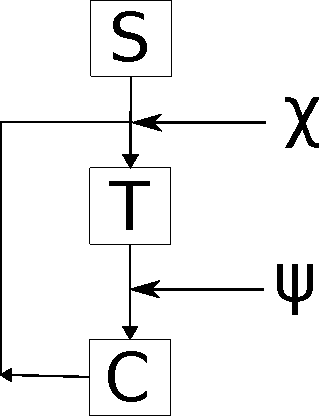
\includegraphics{chapters/random_walk_process_derivation/random_walk_process.pdf}}
    \end{center}
  \caption{\textbf{Monte Carlo random walk procedure for radiation.}
    \textit{A particle state is first sampled from the source distribution. The
      next collision point is sampled from the transport kernel T. Finally,
      the new particle energy and direction is sampled from the collision
      kernel, assuming that an absorption reaction wasn't sampled. If an
      absorption reaction was sampled, the random walk ends. Otherwise, the
      process continues. This procedure allows both the emission density and 
      the collision density to be estimated.}}
  \label{fig:combined_random_walk_process}
\end{figure}

A common modification to the previous analogue random walk processes is to 
ignore absorption. This modification results in the following non-analogue
random walk processes. 
\begin{align}
  \chi(x)\text{ Random Walk (implicit mult.):}&
  \begin{cases}
    p^1(x) & = \frac{S(x)}{\int_{\Gamma} S(x)dx} \\
    p(y \to x) &  = \frac{K(y \to x)}{\bar{c}(y)} \\
    p(x) & = 0
  \end{cases} \\
  \psi(x)\text{ Random Walk (implicit mult.):}&
  \begin{cases}
    p^1(x) & = \frac{S_c(x)}{\int_{\Gamma} S_c(x)dx} \\
    p(y \to x) & = \frac{L(y \to x) }{c(y)} \\
    p(x) & = 0
  \end{cases} \\
  \nonumber \\
  \chi(x)\text{ Random Walk (explicit mult.):}&
  \begin{cases}
    p^1(x) & = \frac{S(x)}{\int_{\Gamma} S(x)dx} \\
    p(y \to x) &  = \frac{K(y \to x)}{\overline{P}_{NA}(x)} \\
    p(x) & = 0
  \end{cases}
  \label{eq:mc_random_walk_emission_dens_nonan} \\
  \psi(x)\text{ Random Walk (explicit mult.):} &
  \begin{cases}
    p^1(x) & = \frac{\psi_1(x)}{\int_{\Gamma}\psi_1(x)dx} \\
    p(y \to x) & = \frac{L(y \to x)}{P_{NA}(x)} \\
    p(x) & = 0
  \end{cases}
  \label{eq:mc_random_walk_collision_dens_nonan}
\end{align}
Russian roulette will have to be used with these random walk processes to 
force random walks to terminate when the particle weight becomes too small. 

\section{Estimating Responses}
In typical radiation transport problems, the inner product of some 
function $a(\vec{r},E,\hat{\Omega})$ and the flux 
$\varphi(\vec{r},E,\hat{\Omega})$ is desired. If the function 
$a(\vec{r},E,\hat{\Omega})$ is a cross section, the inner product that is 
calculated is often called a material response or reaction rate. Because it is 
challenging to estimate the flux directly using a Monte Carlo random walk 
procedure, equivalent inner products must be constructed that are either in 
terms of the collision density or the emission density. 
\begin{align}
  I & = \int a(\vec{r},E,\hat{\Omega}) \varphi(\vec{r},E,\hat{\Omega}) 
  dVdEd\hat{\Omega} \\
  & = \int b(\vec{r},E,\hat{\Omega}) \psi(\vec{r},E,\hat{\Omega})  
  dVdEd\hat{\Omega} \\
  & = \int c(\vec{r},E,\hat{\Omega}) \chi(\vec{r},E,\hat{\Omega}) 
  dVdEd\hat{\Omega}
\end{align}
Based on the relationship between the collision density and the flux, $b(x)$
must be defined as follows, where $\Sigma_T(x)$ is the total cross section.
\begin{equation}
  b(\vec{r},E,\hat{\Omega}) = \frac{a(\vec{r},E,\hat{\Omega})}
  {\Sigma_T(\vec{r},E)}
  \label{eq:collision_response_function}
\end{equation}
Similarly, the function $c(x)$ must be defined as follows.
\begin{equation}
  c(\vec{r},E,\hat{\Omega}) = \int \frac{a(\vec{r}^{'},E,\hat{\Omega})}
  {\Sigma_T(\vec{r}^{'},E)} T(\vec{r} \to \vec{r}^{'},E,\Omega)dV'
  \label{eq:emission_response_function}
\end{equation}

Clearly, the function $b(\vec{r},E,\hat{\Omega})$ will be easier to evaluate, 
which presents an interesting trade-off. Estimators will be easier to use if 
the random walk process for the collision density is used. However, the random 
walk process for the collision density will be harder to conduct than the 
random walk process for the emission density because of the difficulty in 
evaluating the first collided source. Fortunately, the combined random walk 
process allows one to take advantage of the function 
$b(\vec{r},E,\hat{\Omega})$ without ever having to evaluate the first collided 
source. 

In chapter \ref{ch:mc_methods}, two very general estimators were introduced.
When one is dealing with the transport equation, there is another estimator 
called the track length estimator that can be used. A derivation of this 
estimator, which is a limiting case of the event estimator, can be found in ref.
\citep{spanier_monte_1969}. If the function $a(\vec{r},E,\hat{\Omega})$ is 
assumed to have the following form, then the track length estimator can be 
defined. 
\begin{equation*}
  a(\vec{r},E,\hat{\Omega}) = 
  \begin{cases}
    f(\vec{r},E,\hat{\Omega}) & \text{ if } \vec{r} \in V_d \\
    0 & \text{ o.w.}
  \end{cases}
\end{equation*}

\begin{equation}
  \eta^{*}(\alpha) = \sum_m W_m(\alpha)f_md_m
\end{equation}
The value $d_m$ is simply the length of the $m^{th}$ particle track in the 
volume $V_d$. The value $f_m$ is the value of the function 
$f(\vec{r},E,\hat{\Omega})$ along the $m^{th}$ particle track. 

\blankpage
\chapter{The Monte Carlo Random Walk Process for Adjoint Radiation Transport}
\label{ch:adjoint_particle_transport}
In chapter \ref{ch:mc_methods}, the dual problem for calculating inner products
over small sphase spaces was introduced. In this chapter, it will be shown how
the dual problem can be solved in the context of radiation transport 
problems. This will require both the derivation of the dual problems of interest
and their associated Monte Carlo random walk processes. Since, in the previous
chapter, the FEISKs that described the event densities were shown to have 
ideal random walk PDFs, their dual problems will be evaluated first. The 
random walk process for the more general dual problem, which is characterized
by the adjoint transport equation, will then be determined. 

\section{The Adjoint of the Emission Density FIESK}
Using the procedure outlined in chapter \ref{ch:mc_methods}, the dual emission
density FIESK will be constructed. The function that will solve this dual 
equation will be called the adjoint of the emission density. It is not called
the adjoint emission density because, as will be shown, this function does
not behave like an emission density (or in general an event density). First, 
a linear operator will be constructed from equation 
\ref{eq:emission_density_integral_eqn}, which is the emission density FIESK. 
\begin{equation}
  \begin{split}
    H_{\chi} \cdot &\chi(\vec{r},E,\hat{\Omega}) = 
    \chi(\vec{r},E,\hat{\Omega}) - \\
    & \int\int\int C(\vec{r},E^{'} \to E,\hat{\Omega^{'}} \to \hat{\Omega})
    T(\vec{r^{'}} \to \vec{r},E^{'},\hat{\Omega^{'}}) 
    \chi(\vec{r^{'}},E',\hat{\Omega^{'}}) dV^{'}dE^{'}E\hat{\Omega^{'}}
  \end{split}
\end{equation}
With the operator $H_{\chi}$ defined in this way it is clear from equation
\ref{eq:emission_density_integral_eqn} that 
$H_{\chi} = S(\vec{r},E,\hat{\Omega})$.

To define the adjoint operator, the following equality must hold. Where the 
brackets indicate integration over all phase space.
\begin{equation*}
  \langle \chi^{\dagger}H_{\chi} \cdot \chi \rangle = 
  \langle \chi H_{\chi}^{\dagger} \cdot \chi^{\dagger} \rangle
\end{equation*}
Since the operator $H_{\chi}$ is known, the left bracket will be expanded.
\begin{align}
  \langle \chi^{\dagger}H_{\chi} \cdot \chi \rangle & =
  \int\int\int \
  \chi^{\dagger}(\vec{r},E,\hat{\Omega}) \chi(\vec{r},E,\hat{\Omega})
  dV dE d\hat{\Omega} - \int\int\int \chi^{\dagger}(\vec{r},E,\hat{\Omega}) 
  \nonumber \\
  \cdot \int\int\int 
  C(\vec{r}&,E^{'} \to E, \hat{\Omega^{'}} \to \hat{\Omega^{'}})
  T(\vec{r^{'}} \to \vec{r},E^{'},\hat{\Omega^{'}})
  \chi(\vec{r^{'}},E^{'},\hat{\Omega^{'}}) dV^{'}dE^{'}d\hat{\Omega^{'}}
  dV dE d\hat{\Omega} \nonumber \\
  & = \int\int\int \
  \chi^{\dagger}(\vec{r},E,\hat{\Omega}) \chi(\vec{r},E,\hat{\Omega})
  dV dE d\hat{\Omega} - \int\int\int \chi(\vec{r^{'}},E^{'},\hat{\Omega^{'}}) 
  \nonumber \\
  \cdot \int\int\int 
  C(\vec{r}&,E^{'} \to E, \hat{\Omega^{'}} \to \hat{\Omega^{'}})
  T(\vec{r^{'}} \to \vec{r},E^{'},\hat{\Omega^{'}})
  \chi^{\dagger}(\vec{r},E,\hat{\Omega}) dV dE d\hat{\Omega}
  dV^{'}dE^{'}d\hat{\Omega^{'}}
\end{align}
From this last manipulation, the adjoint operator can be deduced, which is 
shown in the following equation.
\begin{equation}
  \begin{split}
    H_{\chi}^{\dagger} \cdot &\chi^{\dagger}(\vec{r},E,\hat{\Omega}) = 
    \chi^{\dagger}(\vec{r},E,\hat{\Omega}) - \\
    & \int\int\int T(\vec{r} \to \vec{r^{'}},E,\hat{\Omega}) 
    C(\vec{r^{'}},E \to E^{'},\hat{\Omega} \to \hat{\Omega^{'}})
    \chi(\vec{r^{'}},E',\hat{\Omega^{'}}) dE^{'}d\hat{\Omega^{'}}dV^{'}
  \end{split}
\end{equation}

In the previous chapter, the function $c(\vec{r},E,\hat{\Omega})$ was defined 
in equation \ref{eq:emission_response_function}, which should be used with 
the emission density to calculate a response. By forcing the adjoint 
operator acting on the adjoint of the emission density to equal the 
function $c(\vec{r},E,\hat{\Omega})$, the dual equation, or simply the adjoint
of the emission density FIESK can be created.
\begin{equation}
  \begin{split}
    \chi^{\dagger}(\vec{r},&E,\hat{\Omega}) = c(\vec{r},E,\hat{\Omega}) + \\
    &\int\int\int T(\vec{r} \to \vec{r^{'}},E,\hat{\Omega}) 
    C(\vec{r^{'}},E \to E^{'},\hat{\Omega} \to \hat{\Omega^{'}})
    \chi^{\dagger}(\vec{r^{'}},E',\hat{\Omega^{'}}) dE^{'}d\hat{\Omega^{'}}dV^{'}
  \end{split}
  \label{eq:adjoint_of_emission_density_integral_eqn}
\end{equation}

Unfortunately, in the integral in equation 
\ref{eq:adjoint_of_emission_density_integral_eqn}, the transport and collision 
kernels are integrated over what was previously the final states. Therefore,
the properties that were defined for these kernels in the previous chapter are 
no longer valid. In particular, the transport kernel is not normalized anymore
and the collision kernel is not equal to the average number of particles 
emitted from a collision when integrated over all final states. To try and 
simplify these kernels, the $\Sigma_T(\vec{r^{'}},E)$ terms  in both the 
transport and collision kernels will be allowed to cancel each other out. The 
modified tranpsport kernel will now be examined.
\begin{equation}
  \frac{T(\vec{r} \to \vec{r^{'}},E,\hat{\Omega})}{\Sigma_T(\vec{r^{'}},E)} = 
  exp\left[-\int_0^{|\vec{r^{'}} - \vec{r}|} 
    \Sigma_T(\vec{r^{'}} - R^{'} \hat{\Omega},E)dR^{'} \right]
  \frac{\delta \left(\Omega - \left[\frac{\vec{r^{'}} - \vec{r}}
      {|\vec{r^{'}} - \vec{r}|}\right]\right)}
       {|\vec{r^{'}} - \vec{r}|^2}
  \label{eq:unnormalized_adjoint_transport_kernel}
\end{equation}
Based on the argument of the delta function, 
$\hat{\Omega} = \frac{\vec{r^{'}} - \vec{r}}{|\vec{r^{'}} - \vec{r}|}$ and 
therefore, $\vec{r^{'}} = \vec{r} + \hat{\Omega}|\vec{r^{'}} - \vec{r}|$. This
equation for $\vec{r^{'}}$ can be substituted back into the equation
\ref{eq:unnormalized_adjoint_transport_kernel}.
\begin{equation*}
  \frac{T(\vec{r} \to \vec{r^{'}},E,\hat{\Omega})}{\Sigma_T(\vec{r^{'}},E)} = 
  exp\left[-\int_0^{|\vec{r^{'}} - \vec{r}|} 
    \Sigma_T \left(\vec{r} + \left[|\vec{r^{'}} - \vec{r}| - R^{'} \right] 
    \hat{\Omega},E \right) dR^{'} 
    \right] \frac{\delta \left(\Omega - \left[\frac{\vec{r^{'}} - \vec{r}}
      {|\vec{r^{'}} - \vec{r}|}\right]\right)}
       {|\vec{r^{'}} - \vec{r}|^2}
\end{equation*}
A new variable of integration can be defined to simplify the exponent. Note
that when $R^{'} = 0$, $R^{''} = |\vec{r^{'}} - \vec{r}|$ and when 
$R^{'} = |\vec{r^{'}} - \vec{r}|$, $R^{''} = 0$.
\begin{align}
  R^{''} & = |\vec{r^{'}} - \vec{r}| - R^{'} \nonumber \\
  dR^{''} & = -dR^{'} \nonumber 
\end{align}
\begin{align}
  \frac{T(\vec{r} \to \vec{r^{'}},E,\hat{\Omega})}{\Sigma_T(\vec{r^{'}},E)} & =
  exp\left[-\int_0^{|\vec{r^{'}} - \vec{r}|} 
    \Sigma_T \left(\vec{r} + R^{''}\hat{\Omega},E \right) dR^{''} 
    \right] \frac{\delta \left(\Omega - \left[\frac{\vec{r^{'}} - \vec{r}}
      {|\vec{r^{'}} - \vec{r}|}\right]\right)}
       {|\vec{r^{'}} - \vec{r}|^2} \nonumber \\
       & = exp\left[-\int_0^{|\vec{r} - \vec{r^{'}}|} 
    \Sigma_T \left(\vec{r} + R^{''}\hat{\Omega},E \right) dR^{''} 
    \right] \frac{\delta \left(\Omega + \left[\frac{\vec{r} - \vec{r^{'}}}
      {|\vec{r} - \vec{r^{'}}|}\right]\right)}
       {|\vec{r} - \vec{r^{'}}|^2} \nonumber \\
       & = \tau(\vec{r^{'}},\vec{r},E,-\hat{\Omega}) \\
       & = \frac{T(\vec{r^{'}} \to \vec{r},E,-\hat{\Omega})}
       {\Sigma_T(\vec{r},E)}
\end{align}
The complete adjoint of the emission density state transition kernel can now be 
defined.
\begin{equation}
  K^{\dagger}(\vec{r^{'}} \to \vec{r},E^{'} \to E,
  \hat{\Omega^{'}} \to \hat{\Omega}) = 
  \tau(\vec{r^{'}},\vec{r},E,-\hat{\Omega}) 
  \Sigma_T(\vec{r^{'}},E \to E^{'},\hat{\Omega} \to \hat{\Omega^{'}})
\end{equation}
The source term $c(\vec{r},E,\hat{\Omega})$ can also be modified, since it
contains the modified transport kernel.
\begin{eqnarray}
  c(\vec{r},E,\hat{\Omega}) & = & \int \frac{a(\vec{r^{'}},E,\hat{\Omega})}
  {\Sigma_T(\vec{r^{'}},E)}T(\vec{r} \to \vec{r^{'}},E,\hat{\Omega}) dV^{'} 
  \nonumber \\
  & = & \int a(\vec{r^{'}},E,\hat{\Omega}) 
  \tau(\vec{r^{'}},\vec{r},E,-\hat{\Omega}) dV^{'}
\end{eqnarray}
Finally, the adjoint of the emission density FIESK can be rewritten with the 
modifications that were just described.
\begin{equation}
  \begin{split}
    \chi^{\dagger}(\vec{r},E,\hat{\Omega}) =  \int a(\vec{r^{'}},&E,\hat{\Omega}) 
    \tau(\vec{r^{'}},\vec{r},E,-\hat{\Omega}) dV^{'} + \\
    & \int\int\int  \tau(\vec{r^{'}},\vec{r},E,-\hat{\Omega}) 
    \Sigma_T(\vec{r^{'}},E \to E^{'},\hat{\Omega} \to \hat{\Omega^{'}})
    dE^{'}d\hat{\Omega^{'}}dV^{'}
  \end{split}
  \label{eq:adjoint_of_emission_density_integral_eqn_2}
\end{equation}
 
By comparing equation \ref{eq:adjoint_of_emission_density_integral_eqn_2} to 
equation \ref{eq:flux_integral_equation} for the flux, it is clear that
the adjoint of the emission density behaves very similar to the flux. In the 
literature, the adjoint of the emission density is often called ``flux-like'' 
because of this similarity \citep{hoogenboom_adjoint_1977}. Though it will not 
be shown, the adjoint of the collision density is also ``flux-like.'' 
Unfortunetly, it was shown in the previous chapter that the random walk process 
to estimate the flux was not ideal. While a random walk process could be 
constructed for the adjoint of the emission density, because of its flux-like 
nature, its random walk process will not be ideal either. 

One way to construct a function that will be collision like and still retain
the favorable properties of the dual problem (i.e. the response function 
becomes the source) is to multiply equation 
\ref{eq:adjoint_of_emission_density_integral_eqn_2} by some function 
$\Sigma^{*}(\vec{r},E)$, whose only necessary properties are that is is
strictly positive and that it goes to zero in a vacuum. This manipulation and 
several others are shown in appendix \ref{ch:appendix_a}. However, it will be 
more instructive to take a step back and start over again with the adjoint 
transport equation. Then the process for deriving the random walk process for 
the emission density and collision density outlined in the previous chapter 
can be followed. 

\section{The Adjoint Integro-Differential Boltzmann Equation}
The integro-differential transport equation can also be written in an
operator form. In the following equation, it is assumed that the flux 
distribution is time-independent.
\begin{equation}
  H_B \cdot \varphi(\vec{r},E,\hat{\Omega}) = S(\vec{r},E,\hat{\Omega})
\end{equation}
Using the integro-differential transport operator, defined below, and the 
equality shown in equation \ref{eq:forward_adjoint_ops} the adjoint 
integro-differential transport operator can be derived. This derivation is shown
in detail in ref. \citep{lewis_computational_1993}. The function 
$\varphi^{\dagger}(\vec{r},E,\hat{\Omega})$ is the adjoint flux.
\begin{equation}
  \begin{split}
    H_B \cdot \varphi(\vec{r},E,\hat{\Omega}) &= 
    \left[ \hat{\Omega} \cdot \vec{\triangledown} +
     \Sigma_T(\vec{r},E) \right] \varphi(\vec{r},E,\hat{\Omega}) - \\
     & \int\int \Sigma_T(\vec{r},E^{'} \to E,\hat{\Omega^{'}} \to \hat{\Omega})
    \varphi(\vec{r},E^{'},\hat{\Omega^{'}}) dE^{'} d\hat{\Omega^{'}}
  \end{split}
  \label{eq:integro_diff_trans_op}
\end{equation}
\begin{equation}
  \begin{split}
    H_B^{\dagger} \cdot \varphi^{\dagger}(\vec{r},E,\hat{\Omega}) &= 
    \left[ -\hat{\Omega} \cdot \vec{\bigtriangledown} +
     \Sigma_T(\vec{r},E) \right] \varphi^{\dagger}(\vec{r},E,\hat{\Omega}) - \\
     & \int\int \Sigma_T(\vec{r},E \to E^{'},\hat{\Omega} \to \hat{\Omega^{'}})
    \varphi^{\dagger}(\vec{r},E^{'},\hat{\Omega^{'}}) dE^{'} d\hat{\Omega^{'}}
  \end{split}
  \label{eq:integro_diff_adj_trans_op}
\end{equation}

Finally, the adjoint integro-differential transport equation can be derived by
forcing $H_B^{\dagger} \cdot \varphi^{\dagger}(\vec{r},E,\hat{\Omega})$ to equal
the response function $a(\vec{r},E,\hat{\Omega})$. This will ensure that the
inner product of the adjoint flux and the source will give the same value as
the inner product of the flux and the response function.
\begin{equation}
  \begin{split}
    -\hat{\Omega} &\cdot \vec{\bigtriangledown} 
    \varphi^{\dagger}(\vec{r},E,\hat{\Omega},t)
    + \Sigma_T(\vec{r},E) \varphi^{\dagger}(\vec{r},E,\hat{\Omega},t) = \\
    & \quad a(\vec{r},E,\hat{\Omega},t) +
    \int\int \Sigma_T(\vec{r},E \to E^{'},\hat{\Omega} \to \hat{\Omega^{'}})
    \varphi(\vec{r},E^{'},\hat{\Omega^{'}},t) dE^{'}d\hat{\Omega^{'}} 
  \end{split}
  \label{eq:integro_diff_adj_boltzmann_eqn}
\end{equation}

It must be noted that the doubly differential collision cross section in the
adjoint integro-differential transport equation is identical to the one that
appears in the integro-differential transport equation. However, it is now
integrated over final energies and directions (in the context of the 
integro-differential transport equation). Therefore, it is not clear what the 
normalization for the total transfer probability is or equivalently, what the
mean number of adjoint particles emerging per collision is. 

\section{The Adjoint Transport Equation in Integral Form}
In order to use the Monte Carlo random walk process that has been discussed
in the previous two chapters, the integro-differential form of the adjoint
transport equation must be converted to a FIESK. To do this, the adjoint
transport equation will first be simplified by introducing the adjoint emission
density. It is similar to the emission density in that it represents the 
expected density of particles exiting a collision or the source. However, both
the collision mechanics and the source that determine the adjoint emission 
density are different.
\begin{equation}
  \theta^{\dagger}(\vec{r},E,\hat{\Omega}) = a(\vec{r},E,\hat{\Omega}) +
  \int\int \Sigma_T(\vec{r},E \to E^{'},\hat{\Omega} \to \hat{\Omega^{'}})
  \varphi^{'}(\vec{r},E^{'},\hat{\Omega^{'}}) dE^{'}d\hat{\Omega^{'}}
  \label{eq:adjoint_emission_density}
\end{equation}
The reduced adjoint transport equation is shown in the following equation.
\begin{equation}
  -\hat{\Omega} \cdot \vec{\bigtriangledown} 
    \varphi^{\dagger}(\vec{r},E,\hat{\Omega},t)
    + \Sigma_T(\vec{r},E) \varphi^{\dagger}(\vec{r},E,\hat{\Omega},t) =
    \theta^{\dagger}(\vec{r},E,\hat{\Omega})
\end{equation}
  
From the reduced adjoint transport equation, the method of characteristics will
be used to transform it to its integral form. The characteristic for the 
adjoint transport equation is the following parameterized line.
\begin{equation}
  \vec{r^{'}} = \vec{r} + R\hat{\Omega}
  \label{eq:adjoint_characteristic}
\end{equation}
Using equation \ref{eq:adjoint_characteristic} a directional derivative along
the characteristic can be determined.
\begin{align}
  \frac{d}{dR} & = \frac{dx^{'}}{dR}\frac{\partial}{\partial x} +
  \frac{dy^{'}}{dR}\frac{\partial}{\partial y} +
  \frac{dz^{'}}{dR}\frac{\partial}{\partial z} \nonumber \\
  & = \Omega_x \frac{\partial}{\partial x} +
  \Omega_y \frac{\partial}{\partial y} +
  \Omega_z \frac{\partial}{\partial z} \nonumber \\
  & = \hat{\Omega} \cdot \vec{\bigtriangledown}
\end{align}

Using the directional derivative along the characteristic, the transport 
equation can be reduced to a first order ODE, which can be easily solved with 
the integrating factor 
$exp\left[-\int_0^R \Sigma_T(\vec{r}+R^{'}\hat{\Omega},E)dR^{'} \right]$.
\begin{align}
  -\frac{d}{dR}\varphi^{\dagger}(\vec{r^{'}},E,\hat{\Omega}) + 
  \Sigma_T(\vec{r^{'}},E)
  \varphi^{\dagger}(\vec{r^{'}},E,\hat{\Omega}) & = 
  \theta^{\dagger}(\vec{r^{'}},E,\hat{\Omega}) \nonumber \\
  -\frac{d}{dR}\bigg[\varphi^{\dagger}(\vec{r^{'}},E,\hat{\Omega})
    exp\left[-\int_0^R \Sigma_T(\vec{r}+R^{'}\hat{\Omega},E)dR^{'}\right]
    \bigg] & = \nonumber \\
  \theta^{\dagger}(\vec{r^{'}},E,\hat{\Omega})
  &exp\left[-\int_0^R \Sigma_T(\vec{r}+R^{'}\hat{\Omega},E)dR^{'} \right] 
  \nonumber \\
  -\varphi^{\dagger}(\vec{r} + R\hat{\Omega},E,\hat{\Omega})
  exp\left[-\int_0^R \Sigma_T(\vec{r}+R^{'}\hat{\Omega},E)dR^{'}\right] 
  \bigg|_0^{\infty} & = \nonumber \\
  \int_0^{\infty} 
  \theta^{\dagger}(\vec{r} + R\hat{\Omega},E,\hat{\Omega})
  &exp\left[-\int_0^R \Sigma_T(\vec{r}+R^{'}\hat{\Omega},E)dR^{'} \right] dR
  \nonumber 
\end{align}
\begin{equation}
    \varphi^{\dagger}(\vec{r},E,\hat{\Omega}) = 
    \int_0^{\infty} \theta^{\dagger}(\vec{r} + R\hat{\Omega},E,\hat{\Omega})
    exp\left[-\int_0^R \Sigma_T(\vec{r}+R^{'}\hat{\Omega},E)dR^{'} \right] dR
  \label{eq:line_integral_adj_transport_eqn}
\end{equation}

To get to equation \ref{eq:line_integral_adj_transport_eqn} it was assumed that
the adjoint flux goes to zero as R goes to infinity. This line integral will
now be converted to an integral over all space. First, note that 
$R = |\vec{r^{'}} - \vec{r}|$,
$\hat{\Omega} = \frac{\vec{r^{'}} - \vec{r}}{|\vec{r^{'}} - \vec{r}}|$ and
$dV^{'} = R^2dRd\hat{\Omega}$
\begin{equation}
  \begin{split}
    \varphi^{\dagger}(\vec{r},E,\hat{\Omega}) = 
    \int \theta^{\dagger}(\vec{r^{'}},E,\hat{\Omega})
    exp\Big[-\int_0^{|\vec{r^{'}} - \vec{r}|} 
      &\Sigma_T(\vec{r}+R^{'}\hat{\Omega},E)dR^{'} \Big] \\
    &\cdot \frac{\delta \left(\Omega - \left[\frac{\vec{r^{'}} - \vec{r}}
        {|\vec{r^{'}} - \vec{r}|}\right]\right)}
    {|\vec{r^{'}} - \vec{r}|^2} dV^{'}
  \end{split}
  \label{eq:volume_integral_adj_transport_eqn}
\end{equation}

This integral equation for the adjoint flux could be converted to a FIESK with
a similar form to the flux FIESK. However, like the flux, the adjoint flux
FIESK will not be well suited for a Monte Carlo random walk process. Instead,
the adjoint emission density FIESK will be derived.

\section{The Adjoint Emission Density FIESK}
To construct a FIESK for the adjoint emission density equation 
\ref{eq:volume_integral_adj_transport_eqn} must be substituted back into 
equation \ref{eq:adjoint_emission_density}. 
\begin{align}
  \theta^{\dagger}(\vec{r},E,\hat{\Omega}) & = a(\vec{r},E,\hat{\Omega}) +
  \int\int \Sigma_T(\vec{r},E \to E^{'},\hat{\Omega} \to \hat{\Omega^{'}})
  \int \theta^{\dagger}(\vec{r^{'}},E^{'},\hat{\Omega^{'}}) \nonumber \\
  \cdot exp&\left[-\int_0^{|\vec{r^{'}} - \vec{r}|} 
    \Sigma_T(\vec{r}+R^{'}\hat{\Omega^{'}},E^{'})dR^{'} \right]
  \cdot \frac{\delta \left(\Omega^{'} - \left[\frac{\vec{r^{'}} - \vec{r}}
      {|\vec{r^{'}} - \vec{r}|}\right]\right)}
        {|\vec{r^{'}} - \vec{r}|^2} dV^{'} dE^{'} d\hat{\Omega^{'}} \nonumber \\
        \theta^{\dagger}(\vec{r},E,\hat{\Omega}) & = a(\vec{r},E,\hat{\Omega}) +
        \int\int \frac{\Sigma^{\dagger}(\vec{r},E^{'})}{\Sigma_T(\vec{r},E^{'})}
        \frac{\Sigma_T(\vec{r},E \to E^{'},\hat{\Omega} \to \hat{\Omega^{'}})}
             {\Sigma^{\dagger}(\vec{r},E^{'})}
  \int \theta^{\dagger}(\vec{r^{'}},E^{'},\hat{\Omega^{'}}) \nonumber \\
  \cdot \Sigma_T(\vec{r},E^{'}) &exp\left[-\int_0^{|\vec{r^{'}} - \vec{r}|} 
    \Sigma_T(\vec{r}+R^{'}\hat{\Omega^{'}},E^{'})dR^{'} \right]
  \cdot \frac{\delta \left(\Omega^{'} - \left[\frac{\vec{r^{'}} - \vec{r}}
      {|\vec{r^{'}} - \vec{r}|}\right]\right)}
        {|\vec{r^{'}} - \vec{r}|^2} dV^{'} dE^{'} d\hat{\Omega^{'}} \nonumber
\end{align}
\begin{equation}
  \begin{split}
    \theta^{\dagger}(\vec{r},E,\hat{\Omega}) = a(\vec{r},E,\hat{\Omega}) + 
    \int\int&\int P^{\dagger}(\vec{r},E^{'})
    C^{\dagger}(\vec{r},E^{'} \to E,\hat{\Omega^{'}} \to \hat{\Omega}) \\
    & \cdot T^{\dagger}(\vec{r^{'}} \to \vec{r},E^{'},\hat{\Omega^{'}})
    \theta^{\dagger}(\vec{r^{'}},E^{'},\hat{\Omega^{'}})
    dV^{'} dE^{'} d\hat{\Omega^{'}}
  \end{split}
  \label{eq:adj_emission_dens_int_eqn}
\end{equation}

The factor $P^{\dagger}(\vec{r},E^{'})$ is called the adjoint weight factor, which
is defined in the next equation. The adjoint weight factor contains the 
function $\Sigma^{\dagger}(\vec{r},E^{'})$, which will be called the total
macroscopic adjoint cross section. The adjoint weight factor takes into account 
the fact that the total macroscopic cross section is not equal to the total 
macroscopic adjoint cross section. In some literature, this factor is called 
the adjoint non-absorption probability \citep{gabler_amos_2006}. However, as 
will be shown in the coming chapters, this factor is not bounded in the 
interval (0,1) but is instead bounded in the interval (0,$\infty$). It is 
therefore inappropriate to call this factor a probability\footnote{This fact is
noted in the reference that calls the factor the adjoint non-absorption 
probability \citep{gabler_amos_2006}.}.
\begin{equation}
  P^{\dagger}(\vec{r},E) = \frac{\Sigma^{\dagger}(\vec{r},E)}
  {\Sigma_T(\vec{r},E)}
\end{equation}

\begin{equation}
  \Sigma^{\dagger}(\vec{r},E^{'}) = \int\int 
  \Sigma_T(\vec{r},E \to E^{'},\hat{\Omega} \to \hat{\Omega^{'}}) dEd\hat{\Omega}
  \label{eq:total_adjoint_cross_section}
\end{equation}

The kernel $T^{\dagger}(\vec{r^{'}} \to \vec{r},E,\hat{\Omega})$ is called
the adjoint transport kernel, which is defined in the next equation. Like the
transport kernel, the adjoint transport kernel prevents events from being
sampled in a vacuum.
\begin{equation}
  \begin{split}
  T^{\dagger}(\vec{r^{'}} \to \vec{r},E,\hat{\Omega}) = 
  \Sigma_T(\vec{r},E^{'}) exp\Big[-\int_0^{|\vec{r^{'}} - \vec{r}|} 
      \Sigma_T(&\vec{r}+R^{'}\hat{\Omega^{'}},E^{'})dR^{'} \Big] \\
    & \cdot \frac{\delta \left(\Omega^{'} - \left[\frac{\vec{r^{'}} - \vec{r}}
        {|\vec{r^{'}} - \vec{r}|}\right]\right)}
    {|\vec{r^{'}} - \vec{r}|^2}
  \end{split}
\end{equation}
The quantity $T^{\dagger}(\vec{r^{'}} \to \vec{r},E,\hat{\Omega})dV$ can be
interpreted as the probability that an adjoint particle at $\vec{r^{'}}$ with
energy $E$ and direction $\hat{\Omega}$ will have its next collision in volume
element $dV$ at $\vec{r}$.

The kernel $C^{\dagger}(\vec{r},E^{'} \to E,\hat{\Omega^{'}} \to \hat{\Omega})$ is
called the adjoint collision kernel, which is defined in the next equation.
\begin{equation}
  C^{\dagger}(\vec{r},E^{'} \to E,\hat{\Omega^{'}} \to \hat{\Omega}) = 
  \frac{\Sigma_T(\vec{r},E \to E^{'},\hat{\Omega} \to \hat{\Omega^{'}})}
       {\Sigma^{\dagger}(\vec{r},E^{'})}
  \label{eq:adj_collision_kernel}
\end{equation}

The adjoint weight factor, adjoint transport kernel and the adjoint collision
kernel can be combined to create a kernel that characterizes the transition of
an adjoint particle from state $y = (\vec{r^{'}},E^{'},\hat{\Omega^{'}})$ of the 
phase space $\Gamma$ to another state $x = (\vec{r},E,\hat{\Omega})$. This new 
kernel is given in the following equation.
\begin{equation}
  \begin{split}
    M^{\dagger}(\vec{r^{'}} \to \vec{r},E^{'} \to E,\hat{\Omega^{'}} \to \hat{\Omega})
    = C^{\dagger}(\vec{r},E^{'} \to E,&\hat{\Omega^{'}} \to \hat{\Omega})
    P^{\dagger}(\vec{r},E^{'}) \\
    & \cdot T^{\dagger}(\vec{r^{'}} \to \vec{r},E^{'},\hat{\Omega^{'}})
  \end{split}
\end{equation}

The integral equation of the adjoint emission density shown in equation 
\ref{eq:adj_emission_dens_int_eqn} can now be represented as
\begin{equation*}
  \theta^{\dagger}(x) = a(x) + \int_{\Gamma}M^{\dagger}(y \to x) \theta^{\dagger}(y)dy,
\end{equation*}
which is a FIESK.

\section{The Adjoint Collision Density FIESK}
Before taking a closer look at the kernel $M^{\dagger}(y \to x)$, the adjoint
collision density must be defined. It is related to the adjoint flux and the
adjoint emission density by the following equations, which are analogous to
the relationships between the collision density, flux and emission density.
\begin{eqnarray}
  \xi^{\dagger}(\vec{r},E,\hat{\Omega}) & = & \Sigma_T(\vec{r},E)
  \varphi^{\dagger}(\vec{r},E,\hat{\Omega}) \\
  & = & \int T^{\dagger}(\vec{r^{'}} \to \vec{r},E,\hat{\Omega})
  \theta^{\dagger}(\vec{r^{'}},E,\hat{\Omega}) dV^{'}
  \label{eq:adj_collision_dens_to_adj_emission_dens}
\end{eqnarray}

Like the collision density, the adjoint collision density is the density of
particles exiting a collision. Using equation 
\ref{eq:adj_collision_dens_to_adj_emission_dens} and equation 
\ref{eq:adjoint_emission_density} an integral equation for the collision 
density can be derived.
\begin{equation*}
  \xi^{\dagger}(x) = S_c^{\dagger}(x) + \int_{\Gamma} N^{\dagger}(y \to x)
  \xi^{\dagger}(y) dy
\end{equation*}
In this equation $S_c^{\dagger}(x)$ is the adjoint first collided source and
$N^{\dagger}(y \to x)$ is a new kernel that also characterizes the transition
of an adjoint particle from state $y = (\vec{r^{'}},E^{'},\hat{\Omega^{'}})$ of
the phase space gamma to another state $x = (\vec{r},E,\hat{\Omega})$. These
functions are defined in the following equations.
\begin{equation}
  S_c^{\dagger}(\vec{r},E,\hat{\Omega}) = \int 
  T^{\dagger}(\vec{r^{'}} \to \vec{r},E,\hat{\Omega}) a(\vec{r^{'}},E,\hat{\Omega})
  dV^{'}
\end{equation}
\begin{equation}
  \begin{split}
    N^{\dagger}(\vec{r^{'}} \to \vec{r},E^{'} \to E,\hat{\Omega^{'}} \to \hat{\Omega})
    = T^{\dagger}(\vec{r^{'}} \to \vec{r},E,\hat{\Omega})
    C^{\dagger}(\vec{r^{'}},&E^{'} \to E,\hat{\Omega^{'}} \to \hat{\Omega}) \\
    & \cdot P^{\dagger}(\vec{r^{'}},E^{'}) 
  \end{split}
\end{equation}

\section{Adjoint Emission and Collision Density State Transition Kernel Properties}
Before the PDFs that govern the random walk process are derived, the adjoint
transport kernel, adjoint collision kernel and adjoint weight factor must be 
investigated a bit further. A comparison of the adjoint transport kernel and 
the transport kernel reveals that the adjoint transport kernel is identical 
the the transport kernel with $\hat{\Omega} = -\hat{\Omega}$. The significance 
of this relationship is that adjoint particles move in the direction opposite 
of the variable $\hat{\Omega}$. It is therefore inappropriate to interpret the 
variable $\hat{\Omega}$ of an adjoint particle as its direction. However, for 
convenience, it will continue to be refered to as an adjoint particle's 
direction. This relationship also indicates that the adjoint transport kernel
is normalized for an infinite medium.
\begin{equation}
  T^{\dagger}(\vec{r^{'}} \to \vec{r},E,\hat{\Omega}) = 
  T(\vec{r^{'}} \to \vec{r},E,-\hat{\Omega}) 
\end{equation}
\begin{equation}
  \int T^{\dagger}(\vec{r^{'}} \to \vec{r},E,\hat{\Omega}) dV = 1
\end{equation}
In problems where the domain of interest in finite, random walks should be 
terminated when they exit the domain of interest. This procedure was described
in the previous chapter to account for the unnormalized transport kernel in
finite domains. Because of the relationship between the transport kernel and 
the adjoint transport kernel, this procedure is also valid for the adjoint
transport kernel. 

Based on the definition of the adjoint collision kernel from equation
\ref{eq:adj_collision_kernel} and the total adjoint cross section from 
equation \ref{eq:total_adjoint_cross_section}, the adjoint collision kernel is 
also normalized to unity. 
\begin{align}
  \int\int C^{\dagger}(\vec{r},E^{'} \to E,\hat{\Omega^{'}} \to \hat{\Omega})
  dE d\hat{\Omega} & = \int\int 
  \frac{\Sigma_T(\vec{r},E \to E^{'},\hat{\Omega} \to \hat{\Omega^{'}})} 
       {\Sigma^{\dagger}(\vec{r},E^{'})} dEd\hat{\Omega} \nonumber \\
  & = 1 \nonumber 
\end{align}
This property of the adjoint collision kernel holds even if multiplying
reactions are possible in a medium. This means that, regardless of the
type of reaction, only one adjoint particle will be emitted and absorption of
adjoint particles is impossible. Since in adjoint collision, the adjoint
particle will gain energy, the lack of an adjoint absorption reaction makes
sense. The consequence of the lack of an adjoint absorption reaction is that
an analogue random walk process for the adjoint FIESKs is not possible. In
addition, Russian rulette will have to be used to terminate histories.        

As mentioned before, the adjoint weight factor $P^{\dagger}(\vec{r},E)$ takes 
into account the fact that the total macroscopic cross section 
$\Sigma_T(\vec{r},E)$, which is used to normalize the transport kernel, is not 
equal to the total macroscopic adjoint cross section 
$\Sigma^{\dagger}(\vec{r},E)$, which is used to normalize the collision kernel. 
Unfortunately, this factor is not bounded to the interval (0,1), which means
that it is likely to increase the variance of the estimators used. It will be 
shown later that in certain circumstances, a change of variables will actually 
constrain the adjoint weight factor to the interval (0,1). In general, 
understanding the behavior of the adjoint weight factor will be very important 
in predicting the variance of the estimators used in a calculation.

Based on the properties of the adjoint transport kernel, adjoint collision
kernel and the adjoint weight factor, the properties of the adjoint emission
density state transition kernel can be determined. The first property is that
the emission density state transition kernel is always positive. The second
property is that the normalization of the kernel is less than infinity. The
kernel normalization, which is shown below, is 
$\overline{P}^{\dagger}(\vec{r^{'}},E^{'})$. This function can be interpreted as
an average of the adjoint weight factor along the line from $\vec{r^{'}}$ to
$\vec{r}$ given an adjoint particle of energy $E^{'}$.
\begin{align}
  \int M^{\dagger}(y \to x)dx & = \int\int\int 
  C^{\dagger}(\vec{r},E^{'} \to E,\hat{\Omega^{'}} \to \hat{\Omega})
  P^{\dagger}(\vec{r},E^{'}) 
  T^{\dagger}(\vec{r^{'}} \to \vec{r},E^{'},\hat{\Omega^{'}}) dE d\hat{\Omega}) dV
  \nonumber \\
  & = \int P^{\dagger}(\vec{r},E^{'})
  T^{\dagger}(\vec{r^{'}} \to \vec{r},E^{'},\hat{\Omega^{'}}) dE d\hat{\Omega}) dV
  \nonumber \\
  & = \overline{P}^{\dagger}(\vec{r^{'}},E^{'}) 
\end{align}

The properties of the adjoint collision density state transition can also be
determined. Like the adjoint emission density state transition kernel, the 
collision density state transition kernel is always positive. The kernel
normalization, which is shown below, is the adjoint weight factor 
$P^{\dagger}(\vec{r^{'}},E^{'})$. 
\begin{align}
  \int N^{\dagger}(y \to x)dx & = \int\int\int
  T^{\dagger}(\vec{r^{'}} \to \vec{r},E,\hat{\Omega})
  C^{\dagger}(\vec{r^{'}},E^{'} \to E,\hat{\Omega^{'}} \to \hat{\Omega})
  P^{\dagger}(\vec{r^{'}},E^{'}) dV dE d\hat{\Omega}) 
  \nonumber \\
  & = \int C^{\dagger}(\vec{r^{'}},E^{'} \to E,\hat{\Omega^{'}} \to \hat{\Omega})
  P^{\dagger}(\vec{r^{'}},E^{'}) dE d\hat{\Omega})
  \nonumber \\
  & = P^{\dagger}(\vec{r^{'}},E^{'}) 
\end{align}

The properties of the two state transition kernels are summarized below. 
\begin{enumerate}
  \item $M^{\dagger}(y \to x) > 0$ \\
    $N^{\dagger}(y \to x) > 0$
  \item $\int M^{\dagger}(y \to x)dx = \overline{P}^{\dagger}(y) < \infty$ \\
    $\int N^{\dagger}(y \to x)dx = P^{\dagger}(y) < \infty$
\end{enumerate}

Based on these properties for the two kernels and the fact that the adjoint
survival probability is always unity due to the lack of an absorption reaction,
it is clear that an analogue random walk process for adjoint radiation 
transport is impossible. Despite this fact, it will still be useful to conduct 
an indirect sampling of the state transition kernels, which will be discussed in
the next section. 

\section{Indirect Sampling of the Adjoint Collision Kernel}
As explained in the previous chapter, the total transfer probability, which
appears in both the collision kernel and the adjoint collision kernel, is
challenging to obtain and even more challenging to sample from. To conduct
the random walks for adjoint radiation, the adjoint collision kernel 
must be sampled indirectly. The adjoint collision will be expanded in order
to determine this sampling procedure. 
\begin{align}
  C^{\dagger}(\vec{r},E^{'} \to E,\hat{\Omega^{'}} \to \hat{\Omega}) & =
  \frac{\Sigma_T(\vec{r},E \to E^{'},\hat{\Omega} \to \hat{\Omega^{'}})}
       {\Sigma^{\dagger}(\vec{r},E^{'})} \nonumber \\
       & = \sum_j 
       \frac{\Sigma_{j}(\vec{r},E)c_j(\vec{r},E)
         f_j(E \to E^{'},\hat{\Omega} \to \hat{\Omega^{'}})}
            {\Sigma^{\dagger}(\vec{r},E^{'})} \nonumber \\
  & = \sum_A \frac{\Sigma_A^{\dagger}(\vec{r},E^{'})}
                  {\Sigma^{\dagger}(\vec{r},E^{'})}
  \sum_j \frac{\sigma_{A,j}^{\dagger}(E^{'})}{\sigma_A^{\dagger}(E^{'})}
  \frac{\sigma_{A,j}(E) c_{A,j}(E) 
        f_{A,j}(E \to E^{'},\hat{\Omega} \to \hat{\Omega^{'}})}
       {\sigma_{A,j}^{\dagger}(E^{'})} \nonumber \\
  & = \sum_A p_A^{\dagger}(\vec{r},E^{'}) \sum_j p_{A,j}^{\dagger}(E^{'})
       f_{A,j}^{\dagger}(E^{'} \to E,\hat{\Omega^{'}} \to \hat{\Omega})
  \label{eq:expanded_adj_collision_kernel}
\end{align}
In this expansion, the subscript A denotes a particular nuclide and the
subscript j denotes a particular type of reaction. The doubly differential
transfer probability $f_{A,j}(E \to E^{'},\hat{\Omega} \to \hat{\Omega^{'}})$
is no longer normalized and connot be used as a PDF for sampling the outgoing
adjoint particle energy and direction. However, as indicated in equation
\ref{eq:expanded_adj_collision_kernel} a new doubly differential transfer
probability can be constructed for adjoint particles. 
\begin{equation}
  f_{A,j}^{\dagger}(E^{'} \to E,\hat{\Omega^{'}} \to \hat{\Omega}) = 
  \frac{\sigma_{A,j}(E)c_{A,j}(E) 
    f_{A,j}(E \to E^{'},\hat{\Omega} \to \hat{\Omega^{'}})}
       {\sigma_{A,j}^{\dagger}(E^{'})}
\end{equation}
The microscopic adjoint cross section for reaction $j$ with nuclide $A$ will
be defined as follows.
\begin{equation}
  \sigma_{A,j}^{\dagger}(E^{'}) = \int\int
  \sigma_{A,j}(E)c_{A,j}(E) 
    f_{A,j}(E \to E^{'},\hat{\Omega} \to \hat{\Omega^{'}}) dE d\hat{\Omega^{'}}
\end{equation}
Therefore, the adjoint doubly differential transfer probability is indeed 
normalized to unity.
\begin{equation}
  \int\int f_{A,j}^{\dagger}(E^{'} \to E,\hat{\Omega^{'}} \to \hat{\Omega})
  dE d\hat{\Omega} = 1
\end{equation}

The process of indirectly sampling the collision kernel is now completely 
defined by equation \ref{eq:expanded_adj_collision_kernel}. In this process,
one first samples the nuclide hit from the discrete PDF 
$p_A^{\dagger}(\vec{r},E^{'})$. With the nuclide A chosen, the reaction type is
sampled from the discrete PDF $p_{A,j}^{\dagger}(E^{'})$. Finally, the outgoing
energy and direction is sampled from the adjoint transfer probability
$f_{A,j}^{\dagger}(E^{'} \to E,\hat{\Omega^{'}} \to \hat{\Omega})$. 

To use this process, one must be able to calculate the microscopic adjoint
cross sections and the adjoint doubly differential transfer probabilities. 
These calculations will be discussed in the next chapter. 

\section{The Adjoint Emission Density and Adjoint Collision Density Random Walk PDFs}
With the state transition kernels $M^{\dagger}(y \to x)$ and 
$N^{\dagger}(y \to x)$ fully characterized, the Monte Carlo random walk process
for adjoint radiation can be completely specified. 
\begin{align}
  \theta^{\dagger}(x)\text{ Random Walk:}&
  \begin{cases}
    p^1(x) & = \frac{a(x)}{\int_{\Gamma} a(x)dx} \\
    p(y \to x) & = \frac{M^{\dagger}(y \to x)}{\overline{P}^{\dagger}(y)} \\
    p(x) & = 0
  \end{cases}
  \label{eq:mc_random_walk_adj_emission_dens} \\
  \xi^{\dagger}(x)\text{ Random Walk:}&
  \begin{cases}
    p^1(x) & = \frac{S_c^{\dagger}(x)}{\int_{\gamma} S_c^{\dagger}(x)dx} \\
    p(y \to x) & = \frac{N^{\dagger}(y \to x)}{P^{\dagger}(y)} \\
    p(x) & = 0
  \end{cases}
  \label{eq:mc_random_walk_adj_collision_dens}
\end{align}

While it might appear from the above PDFs that the two random walk processes
for the adjoint emission and collision densities are completely different,
because the kernels $M^{\dagger}(y \to x)$ and $N^{\dagger}(y \to x)$ only differ
in the ordering of the adjoint tansport kernel, adjoint collision kernel and 
adjoint weight factor, both of these quantities can be estimated during the
same random walk process. Figure \ref{fig:combined_adj_random_walk_process}
illustrates the new combined random walk process. In this new process, 
particles always start in the true adjoint source and not the adjoint first
collided source, which is advantageous because the adjoint first collided 
source would be challenging to calculate. The adjoint emission density will
always be right after a collision (or birth) and the collision density will
alwyas be estimated right before a collision and before multiplying the particle
weight by the adjoint weight factor. This combined process will also prove
advantageous when using either of the estimators that were described in chapter
\ref{ch:mc_methods}. The next section will elaborate on this point.
\begin{figure}[t!]
  \begin{center}
    \scalebox{0.75}{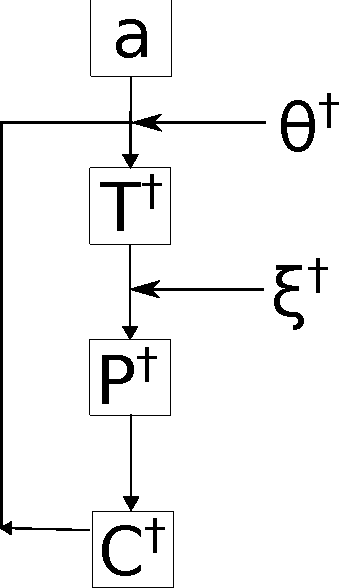
\includegraphics{chapters/adjoint_random_walk_process_derivation/random_walk_process.pdf}}
    \end{center}
  \caption{\textbf{Monte Carlo random walk procedure for adjoint radiation.}
    \textit{A particle state is first sampled from the adjoint source 
      distribution. The next collision point is sampled from the adjoint 
      transport kernel $T^{\dagger}$. Next, the adjoint particle weight is
      multiplied by the adjoint weight factor $P^{\dagger}$. Finally, the new 
      energy and direction is sampled from the adjoint collision kernel. This
      process continues until Russian roulette forces the random walk to
      terminate. This procedure allows both the adjoint emission density and 
      the adjoint collision density to be estimated.}}
  \label{fig:combined_adj_random_walk_process}
\end{figure}

\section{Estimating Responses}
Due to the way that the adjoint transport equation is constructed, the inner
product of the adjoint flux $\varphi^{\dagger}(\vec{r},E,\hat{\Omega})$ and the
source $S(\vec{r},E,\hat{\Omega})$ will result in the same value as the inner 
product of the flux $\varphi(\vec{r},E,\hat{\Omega})$ and the response
function $a(\vec{r},E,\hat{\Omega})$. Because it is not ideal to estimate the
adjoint flux directly using a Monte Carlo random walk procedure, equivalent
inner products must be constructed that are either in terms of the adjoint
collision density or the adjoint emission density.
\begin{eqnarray}
  I & = & \int S(\vec{r},E,\hat{\Omega})\varphi^{\dagger}(\vec{r},E,\hat{\Omega})
  dV dE d\hat{\Omega} \\ 
  & = & \int U(\vec{r},E,\hat{\Omega})\xi^{\dagger}(\vec{r},E,\hat{\Omega})
  dV dE d\hat{\Omega} \\
  & = & \int V(\vec{r},E,\hat{\Omega})\theta^{\dagger}(\vec{r},E,\hat{\Omega})
  dV dE d\hat{\Omega} \\
\end{eqnarray}
Based on the relationship between the adjoint collision density and the
adjoint flux, $U(\vec{r},E,\hat{\Omega})$ must be defined as follows.
\begin{equation}
  U(\vec{r},E,\hat{\Omega}) = \frac{S(\vec{r},E,\hat{\Omega})}
                                   {\Sigma_T(\vec{r},E,\hat{\Omega})}
\end{equation}
Similarly, the function $V(\vec{r},E,\hat{\Omega})$ must be defined as follows.
\begin{eqnarray}
  V(\vec{r},E,\hat{\Omega}) & = & \int \frac{S(\vec{r^{'}},E,\hat{\Omega})}
  {\Sigma_T(\vec{r^{'}},E,\hat{\Omega})} 
  T^{\dagger}(\vec{r} \to \vec{r^{'}},E,\hat{\Omega}) \\
  & = & \frac{S_c(\vec{r},E,\hat{\Omega})}{\Sigma_T(\vec{r},E)}
\end{eqnarray}

Clearly, the function $U(\vec{r},E,\hat{\Omega})$ will be easier to evaluate,
which presents an interesting trade-off. Estimators will be easier to use if
the random walk process for the adjoint collision density is used. However, 
the random walk process for the adjoint collision density will be harder to 
conduct than the random walk process for the adjoint emission density because
of the difficulty in evaluating the adjoint first collided source. Fortunately,
the combined random walk process allows one to take advantage of the function
$U(\vec{r},E,\hat{\Omega})$ without ever having to evaluate the adjoint first 
collided source. Using the track length estimator described in the previous
chapter, the adjoint flux can also be estimated. 

\blankpage
\chapter{Photon Interaction Cross Sections and Sampling Techniques}
\label{ch:photon_interactions}
In the previous two chapters, the Monte Carlo random walk process for both
neutral and charged radiation was described. An important part of the random
walk process is the indirect sampling of the collision kernel, which requires
information on the differential interaction cross sections for the particle
of interest. In this chapter, four primary interactions of high energy photons 
with matter will be discussed: incoherent scattering, coherent scattering, 
pair production and the photoelectric effect. Photonuclear absorption, which can
become important in high energy coupled neutron-photon transport simulations, 
will be discussed briefly. In addition, sampling procedures that can be used 
with each differential interaction cross section will be discribed. All 
secondary particles other than photons will be neglected from the cross sections
and sampling procedures. 

\section{Incoherent Scattering}
Incoherent or Compton scattering occurs when a photon scatters off of an orbital
electron and loses some of its energy. The energy of the liberated electron
is equal to the energy lost by the photon minus the binding energy of the
shell the electron occupied. The differential incoherent scattering cross
section (per atom) is usually expressed as the product of the differential 
Klein-Nishina scattering cross section per electron and the incoherent 
scattering function. Klein and Nishina developed the differential cross section
under the assumption that the electron on which the photon scatters is free 
and at rest \citep{klein_uber_1929}. The incoherent scattering function is the 
correction to the Klein-Nishina scattering cross section from electron binding. 
The differential incoherent scattering cross section is shown below 
\citep{lux_monte_1991}. The value $r_e^2$ is the classical radius of the 
electron and $\alpha^{'}$ is the energy of the incident photon in units of 
electron rest energy.
\begin{align}
  \frac{d\sigma_{i.s.}(\alpha^{'},\theta,Z)}{d\Omega} & = 
  \frac{d\sigma_{K.N.}(\alpha^{'},\theta)}{d\Omega}S(y,Z) \nonumber \\
  & = \frac{r_e^2}{2}
  \frac{\left[1 + \cos{^{2}\theta} + \frac{\alpha^{'2}(1-\cos{\theta})^2}
                                  {1 + \alpha^{'}(1-\cos{\theta})}\right] }
  {\left[1 + \alpha^{'}(1-\cos{\theta}) \right]^2}
  S(y,Z)
  \label{eq:incoh_scat_theta}
\end{align}
The arguments of the scattering function are 
$y = sin(\frac{\theta}{2})/\lambda^{'}$ and $Z$, the atomic number. The 
differential incoherent cross section will sometimes be expressed in terms of 
the outgoing photon energy as well. The alpha variables are simply the photon
energy divided by the rest mass of the electron.
\begin{equation}
  \frac{d\sigma_{i.s.}(\alpha^{'},\theta,Z)}{d\Omega} = \frac{r_e^2}{2}
  \left(\frac{\alpha}{\alpha^{'}} \right)^2
  \left[ \frac{\alpha}{\alpha^{'}} + \frac{\alpha^{'}}{\alpha} - 1 + 
    \cos{^2\theta} \right] S(y,Z)
\end{equation}
The later form of the differential incoherent cross section is made possible 
by the one-to-one correspondance between the outgoing energy and outgoing 
direction, which can be found using conservation of energy and momentum and the 
assumption that the electron is free and at rest (see Appendix 
\ref{ch:appendix_B}). 
\begin{equation}
  E = \frac{E^{'}}{1 + \frac{E^{'}}{m_ec^2}(1 - \cos{\theta})}
\end{equation}
When binding effects cannot be neglected, which typically occurs when the 
incident photon energies are on the order of the electron binding energy, there 
will no longer be a one-to-one correspondance between the outgoing energy and 
the outgoing direction. Instead, there will be a distribution of outgoing 
energies that correspond to each outgoing direction. This phenomenon will be 
discussed more in the next section.

A PDF for the outgoing photon angle can be created by dividing the differential
incoherent cross section by the total incoherent cross section at the incoming
photon energy. Then, by reorganizing the PDF, the procedure for sampling an
outgoing photon direction and energy can be determined 
\citep{persliden_monte_1983}.
\begin{align}
  p(\alpha^{'},\theta,Z) & = \frac{1}{\sigma_{i.s.}(\alpha^{'},Z)}
  \frac{d\sigma_{i.s.}(\alpha^{'},\theta,Z)}{d\Omega} \nonumber \\
  & = \frac{S_{max}(y,Z) \sigma_{K.N.}(\alpha^{'})}{\sigma_{i.s.}(\alpha^{'},Z)}
  \left[ \frac{S(y,Z)}{S_{max}(y,Z)} \right]
  \left[ \frac{1}{\sigma_{K.N.}(\alpha^{'})} 
    \frac{d\sigma_{K.N.}(\alpha^{'},\theta)}
         {d\Omega} \right] \nonumber \\
  & = C(\alpha^{'},Z) R(y,Z) p_{K.N.}(\alpha^{'},\theta) 
\end{align}
The scattering function increases monotonically from 0 when $y=0$ to Z when
$y=\infty$ and therefore,
\begin{equation*} 
S_{max}(y,Z) = S(y_{max},Z).
\end{equation*}
The maximum value of $y$, which occurs when $\theta = \pi$ (corresponding to
back scattering), is simply the inverse wavelength of the incoming 
particle (usually in $cm^{-1}$). Now, to sample the outgoing direction, one 
first samples an angle from the PDF for Compton Scattering off of a free 
electron, $p_{K.N.}(\alpha,\theta)$. Then one uses the rejection function R(y,Z)
with the sampled angle to determine if it should be accepted or rejected. 
Several sampling techniques that can be used with the Klein-Nishina cross 
section will now be discussed.

For the purpose of sampling, it is useful to write the differential 
Klein-Nishina cross section in terms of a new variable whose inverse is the 
energy loss ratio.
\begin{align}
  \frac{1}{x} & = \frac{\alpha}{\alpha^{'}} \\
  & = \frac{1}{1+\alpha^{'}(1-\cos{\theta})}
\end{align}
The differential Klein-Nishina cross section can then be written as follows 
\citep{lux_monte_1991}.
\begin{align}
  \frac{d\sigma_{K.N.}(\alpha^{'},x)}{dx} & = K \left[ A + \frac{B}{x} +
    \frac{C}{x^2} + \frac{D}{x^3} \right] \\
  K & = \frac{\pi r_e^2}{\alpha^{'}} \nonumber \\
  A & = \frac{1}{\alpha^{'2}} \nonumber \\
  B & = 1 - \frac{2(\alpha^{'} + 1)}{\alpha^{'2}} \nonumber \\
  C & = \frac{1 + 2\alpha^{'}}{\alpha^{'2}} \nonumber \\
  D & = 1 \nonumber
\end{align}
The change of variables is carried out in Appendix \ref{ch:appendix_B}.

Now, a PDF for $x$ can be created if the differential Klein-Nishina cross 
section is divided by the total Klein-Nishina cross section, which can be found 
by integrating the differential Klein-Nishina cross section from $x_{min} = 1$ to
$x_{max} = 1 + 2 \alpha^{'}$\footnote{The equation found in Lux and Koblinger's
text book contains an error which is described in Appendix \ref{ch:appendix_B}}.
\begin{equation}
  \sigma_{K.N.}(\alpha^{'}) = 2\pi r_e^2 \left( \frac{1+\alpha^{'}}{\alpha^{'2}}
  \left[\frac{2+2\alpha^{'}}{1+2\alpha^{'}} - 
    \frac{ln(1+2\alpha^{'})}{\alpha^{'}} \right]
  + \frac{ln(1+2\alpha^{'})}{2\alpha^{'}} - 
  \frac{1+3\alpha^{'}}{(1+2\alpha^{'})^2} \right)
\end{equation}
At low photon energies, the evaluation of this equation for the Klein-Nishina 
cross sections can lead to numerical errors due to the near-cancellation between
logarithmic and algebraic terms \citep{lux_monte_1991}. An empirical formula
was created that is correct to within $1.3\%$ up to 100 MeV
\citep{hastings_approximations_1955}. Due to the sampling techniques that will
be used, the total Klein-Nishina cross section will only need to be evaluated
when the incoming photon energy is above about $1.4$ MeV. Therefore there is no 
need to use the empirical formula.

The PDF for $x$ can be defined as follows.
\begin{align}
  p_{K.N.}(\alpha^{'},x) & = 
  \begin{cases}
    H \cdot \left[ A + \frac{B}{x} + \frac{C}{x^2} + \frac{D}{x^3} \right]
    & \text{if } 1 \leq x \leq 1 + 2 \alpha^{'} \\
    0 & \text{o.w.}
  \end{cases} \\
  H & = \frac{K}{\sigma_{K.N.}(\alpha^{'})} \nonumber 
\end{align}
A direct inversion of this PDF is not possible. However, this PDF can still be
sampled directly by using a combination of the probability mixing method and the
inverse CDF method \citep{koblinger_direct_1975}\footnote{For a description of 
all sampling methods that one can use, please refer to refs. \citep{koblinger_direct_1975, lux_monte_1991, spanier_monte_1969, blomquist_assessment_1983}.}. To
use these two sampling techniques, the PDF must be split into four terms. 
\begin{align}
  p_{K.N.}(\alpha^{'},x) = p_1(\alpha^{'},x) + p_2&(\alpha^{'},x) +
  p_3(\alpha^{'},x) + p_4(\alpha^{'},x) \\
  p_1(\alpha^{'},x) & = HA \nonumber \\
  p_2(\alpha^{'},x) & = \frac{HB}{x} \nonumber \\
  p_3(\alpha^{'},x) & = \frac{HC}{x^2} \nonumber \\
  p_4(\alpha^{'},x) & = \frac{HD}{x^3} \nonumber 
\end{align}
Now the $i^{th}$ term can be selected with the following probability.
\begin{equation}
  p_i = \int_1^{1+2\alpha^{'}} p_i(\alpha^{'},x) dx
\end{equation}
For the four functions above, the probabilities of being selected are shown
below. Take note that these probabilities contain the total Klein-Nishina
cross section.
\begin{equation}
  p_i = 
  \begin{cases}
    \frac{2H}{\alpha^{'}} & \text{if } i = 1 \\
    H \left[1 - \frac{2+2\alpha^{'}}{\alpha^{'2}} \right] ln(1 + 2\alpha^{'}) 
    & \text{if } i = 2 \\
    \frac{2H}{\alpha^{'}} & \text{if } i = 3 \\
    \frac{H}{2} \left[1 - \frac{1}{(1+2\alpha^{'})^2} \right] & \text{if } i = 4
    \end{cases}
\end{equation}
In order for this method to work, all of the probabilities must be positive.
Therefore, $p_2$ and $p_4$ impose limits on the values of $\alpha^{'}$ where this
method can be used. The probability $p_2$ is the more restrictive of the two.
When the value of $\alpha^{'}$ is less than $(1 + \sqrt{3})$, $p_2$ will be 
negative and the method cannot be used. This corresponds to a photon energy of
about $1.4$ MeV. Below this energy another method must be used, which will be 
discussed shortly. Once an $i$ has been selected, the value of $x$ is sampled
from the inverse CDF of $p_i(\alpha^{'},x)$. The inverse CDFs for each of the
four functions is shown below. The uniform random number in the interval (0,1)
required by the inverse CDF method is represented by the variable 
$\varepsilon$.
\begin{align}
  P_1^{-1}(\alpha^{'},\varepsilon) & = 1 + 2\alpha^{'}\varepsilon \\
  P_2^{-1}(\alpha^{'},\varepsilon) & = (1 + 2\alpha^{'})^{\varepsilon} \\
  P_3^{-1}(\alpha^{'},\varepsilon) & = \frac{1 + 2\alpha^{'}}
  {1 + 2\alpha^{'}\varepsilon} \\
  P_4^{-1}(\alpha^{'},\varepsilon) & = \left[1 - \varepsilon\left(1 - 
    \frac{1}{(1 + 2\alpha^{'})^2} \right) \right]^{-\frac{1}{2}}
\end{align}
Evaluating the inverse CDF with a random number yields a value of x from the
Klein-Nishina differential cross section. The value of x can then be used to
determine the new energy and direction (relative to the current direction) of 
the photon.
\begin{align}
  \alpha & = \frac{\alpha^{'}}{x} \\
  \cos{\theta} & = 1 + \frac{1-x}{\alpha^{'}} 
\end{align}

When the energy of the incoming photon drops below 1.4 MeV, the rejection
method can be used to sample values of x from the Klein-Nishina cross section.
Kahn developed a rejection sampling procedure that can be used for any incoming
photon energy. However the efficiency of the procedure is highest at lower 
energies \citep{lux_monte_1991, kahn_applications_1956}. This procedure is
shown in figure \ref{fig:kahn_rejection_sampling}.
\begin{figure}[t!]
  \begin{center}
    \def\svgwidth{300bp}
    \input{chapters/photon_interactions/Kahn_sampling_method.pdf_tex}
  \end{center}
  \caption{\textbf{Kahn's Rejection Sampling Procedure}.
    \textit{This sampling procedure is used to sample a value of x from the
    differential Klein-Nishina cross section. One can use this sampling
    procedure at any incoming particle energy, however the efficiency of the
    procedure degrades at higher enegies \citep{lux_monte_1991}.}}
  \label{fig:kahn_rejection_sampling}
\end{figure}

When the direct sampling method and the rejection method are used together, one 
can efficiently sample values from the Klein-Nishina cross section at any 
incoming photon energy. Figure \ref{} shows the efficiency of both Kahn's 
rejection sampling procedure and the combined sampling procedure. At around
1.4 MeV, the efficiency of the combined sampling procedure jumps to one because
of the switch to the direct sampling method. This is a considerable improvement
compared to only using Kahn's method. 

\section{Doppler Broadening of Incoherently Scattered Photons}
As mentioned in the previous section, the differential Klein-Nishina cross 
section assumes that the electron upon which the photon scatters is free
and at rest. Atomic electrons are bound and consequently cannot be at rest. 
When the energy of the incoming photon is much greater than the binding 
energies of the electrons in the atom, binding effects are negligable and the
incoherent cross section becomes simply the atomic number times the 
Klein-Nishina cross section. However, when the incoming photon energy is on the
order of a few hundred keV or lower, binding effects must be taken into account
\citep{namito_implementation_1994}. Taking binding effects into account results
in three significant changes to the simulated transport process. First, electron
binding results in a reduction in the total incoherent cross section, which
in turn results in larger mean free paths for the photon as it travels through
the medium. This occurs because part of the differential cross section is
suppressed because it would result in energetically impossible scattering 
events\footnote{Because the atomic system is a quantum-mechanical system, enough
energy must be given to the electron to free it. Otherwise a reaction will not
occur}. Second, the angular distribution of the scattered photon is 
modified, particurily in the forward direction. Finaly, the Compton-scattered
photon energy is broadened by the pre-collision motion of the electron 
\citep{namito_implementation_1994}. In other words, the one-to-one 
correspondence between the outgoing photon direction and energy is broken and 
for each outgoing direction, there is an associated distribution of outgoing 
photon energies. The first two changes were taken into account in the last
section by multiplying the differential Klein-Nishina cross section by the 
scattering function. In this section, the energy distribution will be dealt
with. 

To take into account the energy distribution, the double differential
incoherent scattering cross section must be used. Using the Born and impulse
approximations, Ribberfors was able to derive the double differential
incoherent scattering cross section, which is shown below 
\citep{ribberfors_x-ray_1983}. This double differential cross section is given 
for each subshell of the atom. The value $\alpha_c$ is called the Compton line, 
which is the outgoing photon energy (divided by the electron rest mass) 
corresponding to the outgoing scattering angle assuming that the electron was 
stationary and free. The variable $\alpha$ is the true outgoing photon 
energy resulting from the collision with a bound, moving electron.
\begin{equation}
  \left(\frac{d^2\sigma(\alpha,\alpha^{'},\theta,Z)}{d\Omega dE}\right)_i = 
  \frac{r_e^2}{2c\left|\vec{\alpha^{'}} - 
    \vec{\alpha}\right|} \left(\frac{\alpha}{\alpha^{'}}\right) 
  \left(\frac{\alpha^{'}}{\alpha_c} + \frac{\alpha_c}{\alpha^{'}} - 1 + 
  cos^2\theta \right) J_i(p_z,Z)
\end{equation}
The function $J_i(p_z,Z)$ is the Compton profile for the $i^{th}$ electron 
subshell for element $Z$. The argument $p_z$ is the projection of the 
electron's initial momentum on the scattering vector 
$\vec{\alpha^{'}} - \vec{\alpha}$. Because of the quantum mechanical nature of 
the atomic system, the electrons in each subshell have an associated 
probability distribution in momentum space, which is often denoted 
$n_i(\vec{p},Z)$. The Compton profile is simply the projection of this 
probability distribution along the scattering vector 
\citep{cooper_compton_1985}.
\begin{equation}
  J_i(p_z,Z) = \int_{p_x} \int_{p_y} n_i(p_x,p_y,p_z,Z)dp_xdp_y
\end{equation}

For the purposes of sampling from this double differential cross section it
will be more useful to do a change of variables from outgoing energy to 
electron momentum projection $p_z$. Using conservation of energy and momentum,
an equation for the electron momentum projection can be determined. This
derivation is shown in Appendix \ref{ch:appendix_B}. 
\begin{align}
  p_z & = m_ec \frac{\alpha - \alpha^{'} + \alpha^{'}\alpha(1 - \cos{\theta})}
  {\left|\vec{\alpha^{'}} - \vec{\alpha}\right|} \nonumber \\
  & = m_ec \frac{\alpha - \alpha^{'} + \alpha^{'}\alpha(1 - \cos{\theta})}
  {\sqrt{\alpha^{'2} + \alpha^{2} - 2\alpha^{'}\alpha^{'2}cos{\theta}}}
  \label{eq:pz}
\end{align}
The derivative of this equation with respect to the outgoing photon energy
is shown below.
\begin{equation}
  \frac{dp_z}{d\alpha} = m_ec \frac{1 + \alpha^{'}(1-\cos{\theta})}
  {\left|\vec{\alpha^{'}} - \vec{\alpha} \right|} - 
  p_z \frac{\left(\alpha - \alpha^{'}\cos{\theta} \right)}
  {\left|\vec{\alpha^{'}} - \vec{\alpha} \right|^2}
  \label{eq:diff_pz}
\end{equation}
Ribborfors suggested a simplification to this derivative based on some 
observations about the Compton profiles \citep{ribberfors_x-ray_1983}. First, 
the Compton profiles are even functions. Therefore, the odd moments of $p_z$ 
will be zero. Second, the Compton profiles drop off fairly rapidly so that
the first moment can be approximated as follows. The limit of integration
$p_{i,max}$ will be explained shortly.
\begin{equation}
  \langle p_z \rangle \approx \int_{-\infty}^{p_{i,max}} p_z J(p_z)dp_z = 0
\end{equation}
Therefore, the second term in equation \ref{eq:diff_pz} can be ignored because
it will not contribute significantly to the total incoherent cross section\footnote{In the change of variables $\frac{d\alpha}{dp_z}$ is used. However, 
constructing a Maclaurin series in $p_z$ to first order will give the same result.}.
\begin{equation}
  \frac{dp_z}{d\alpha} = m_ec \frac{1 + \alpha^{'}(1-\cos{\theta})}
  {\left|\vec{\alpha^{'}} - \vec{\alpha} \right|}
  \label{eq:diff_pz_simp}
\end{equation}

Now the change of variables in the double differential cross section can be
completed \citep{ribberfors_x-ray_1983}.
\begin{align}
  \left(\frac{d^2\sigma(p_z,\theta,Z)}{d\Omega dp_z}\right)_i & = 
  \left(\frac{d^2\sigma(\alpha,\alpha^{'},\theta,Z)}{d\Omega dE}\right)_i 
  \frac{dE}{d\alpha}
  \frac{d\alpha}{dp_z} \nonumber \\ 
  & =  \frac{r_e^2}{2} \left(\frac{\alpha\alpha_c}{\alpha^{'2}}\right) 
  \left(\frac{\alpha^{'}}{\alpha_c} + \frac{\alpha_c}{\alpha^{'}} - 1 + 
  cos^2\theta \right) J_i(p_z,Z)
\end{align}

The differential incoherent scattering cross section from the previous section
can be recovered by integrating over all possible electron momentum projections
and by summing up the resulting differential cross section for each shell.
Because $\alpha$ and $p_z$ are related by equation \ref{eq:pz}, this integral
will be quite complicated. Fortunately, Ribberfors has shown that using the
approximation $\alpha_c \approx \alpha$ results in negligable errors in the 
total incoherent scattering cross section \citep{ribberfors_x-ray_1983}. The
limit of integration $p_{i,max}$ is the maximum electron momentum projection
allowed for a compton scattering reaction to occur. This maximum occurs when
the outgoing photon energy is equal to $E - E_{i,b}$, where $E_{i,b}$ is the 
binding energy for the particular subshell. Unfortunately, $p_{i,max}$ is a 
function of $\theta$ so this integral will still be complicated. 
\begin{align}
  \frac{d\sigma(\alpha^{'},\theta,Z)}{d\Omega} & = 
  \frac{r_e^2}{2} \left(\frac{\alpha_c}{\alpha^{'}}\right)^2 
  \left(\frac{\alpha^{'}}{\alpha_c} + \frac{\alpha_c}{\alpha^{'}} - 1 + 
  cos^2\theta \right) \sum_i \int_{-\infty}^{p_{i,max}} J_i(p_z,Z)dp_z \nonumber \\
  & = \left(\frac{d\sigma}{d\Omega}\right)_{K.N.} S^I(y,Z) \nonumber \\
  & = \left(\frac{d\sigma}{d\Omega}\right)_{K.N.} S(y,Z) \nonumber
\end{align}

The scattering function $S^I(y,Z)$ is the scattering function from the
impulse approximation. The scattering function that is given in most tables
and is recommended for use in Monte Carlo codes is based on the Waller-Hartree
theory. Both of these scattering functions have been shown to be in close 
agreement for many elements though, which is why a direct substitution is 
justified \citep{namito_implementation_1994}. 

The method proposed by Namito et al. for sampling an outgoing photon energy
from the double differential incoherent cross section will now be discussed
\citep{namito_implementation_1994}. The first step is to sample an outgoing
scattering angle from the differential incoherent cross section using the 
methods from the previous section. Next, the subshell containing the electron 
upon which the photon will scatter must be sampled. The most accurate
way to sample the subshell would be to create a discrete PDF based on the total
incoherent cross section for each subshell. This data isn't readily available in
the popular tables \citep{cullen_epdl97_1997}. The approximation used by Namito 
et al., which is only truely applicable when the incoming photon energy is much 
greater than the binding energy of the electron, is to sample the electron shell
based on the number of electrons present in each shell (given as $n_i$).
\begin{align}
  p(i) & = \frac{(\sigma_{i.c.})_i}{\sigma_{i.c.}} \nonumber \\
  & \approx \frac{\sigma_{K.N.}n_i}{\sigma_{K.N.}Z} \nonumber \\
  & \approx \frac{n_i}{Z} 
\end{align}
Finally, an outgoing photon energy must be sampled from the double differential 
incoherent cross section. A conditional PDF for the outgoing photon energy can 
be created by dividing the double differential incoherent cross section by the 
differential coherent cross section evaluated at a particular angle. The value
of $p_{i,max}$ is calculated using the value of $\theta$ that was sampled and
the substitution $\alpha = \alpha^{'}-\frac{E_{i,b}}{m_ec^2}$.
\begin{align}
  p_i(p_z,Z \text{ | } \theta) & = 
  \left(\frac{d\sigma_{i.s.}(\alpha^{'},\theta,Z)}{d\Omega} \right)_i^{-1}
  \left(\frac{d^2\sigma(\alpha,\alpha^{'},\theta,Z)}{d\Omega dp_z}\right)_i 
  \nonumber \\
  & = \left(\frac{\alpha_c\alpha}{\alpha^{'2}}\right)
  \left(\frac{\alpha^{'}}{\alpha_c}\right)^2
  \frac{J_i(p_z,Z)}{S_i(y,Z)} \nonumber \\
  & = (1 + \alpha^{'}\cos{\theta})\left(\frac{\alpha}{\alpha^{'}}\right)
  \left(\frac{J_i(p_z,Z)}{\int_{-\infty}^{p_{i,max}}J_i(p_z,Z)dp_z}\right) \nonumber\\
  & = C(\alpha^{'},\theta)R(\alpha,\alpha^{'})p(p_z,Z)
\end{align}
One must sample a value of $p_z$ from the PDF $p(p_z,Z)$ to determine the
outgoing photon energy. Once the outgoing photon energy has been determined
the rejection function $R(\alpha,\alpha^{'})$ is used to determine if the value 
should be accepted or rejected. The CDF corresponding to the PDF for $p_z$ is 
the following\footnote{Namito et al. actually recommend the CDF $\frac{\int_{0}^{p_z}J_i(x,Z)dx}{\int_{0}^{p_{i,max}}J_i(x,Z)dx}$, which appears to be an error.}.
\begin{equation}
P(p_z,Z) = \frac{\int_{-\infty}^{p_z}J_i(x,Z)dx}{\int_{-\infty}^{p_{i,max}}J_i(x,Z)dx}
\end{equation}
Because the Compton profiles are most commonly found in tabular form\footnote{Biggs et al. have compiled the Compton profiles for atomic numbers 1-102\citep{biggs_hartree-fock_1975}.}, a table method must be used to sample the value of 
$p_z$. One first finds the value of the CDF corresponding to the momentum 
projection $p_{i,max}$. Then one finds the momentum projection associated with 
the CDF value $\varepsilon\int_{-\infty}^{p_{i,max}}J_i(x,Z)dx$, where $\varepsilon$ 
is again a uniform random number. Using a standard binary search algorithm, 
this process can be done very efficiently.

The equation for the outgoing photon energy in terms of the momentum projection
is shown below. When both values are energetically possible, one of the values
must be randomly selected (with probability one half).
\begin{align}
  \alpha & = \frac{-b}{2a} \pm \frac{\sqrt{b^2 - 4ac}}{2a} \\
  a & = \left(\frac{p_z}{m_ec}\right)^2 - 
  \left(\frac{\alpha^{'}}{\alpha_c}\right)^2
  \nonumber \\
  b & = -2\alpha^{'}\left[\left(\frac{p_z}{m_ec}\right)^2\cos{\theta} + 
  \frac{\alpha^{'}}{\alpha_c}\right] \nonumber \\
  c & = \left(\frac{p_z}{m_ec}\right)^2 - 1 \nonumber
\end{align}


\section{Coherent Scattering}
Coherent or Rayleigh scattering occurs when a photon scatters off of an atom 
with negligable energy loss. It occurs rarely except for when low energy (keV)
photons pass through a high atomic number material 
\citep{lux_monte_1991}. The differential coherent cross section (per atom) is 
usually expressed as a product of the classical Thompson differential 
cross section per electron and the atomic form factor squared. The differential 
coherent cross section is shown below \citep{lux_monte_1991}. The value $r_e$ 
is the classical radius of the electron. The arguments of the atomic form factor
are $y = \sin{\frac{\theta}{2}}/\lambda^{'}$ and Z, the atomic number. 
\begin{align}
  \frac{d\sigma_{c.s.}(\alpha^{'},\theta,Z)}{d\Omega} & = 
  \frac{d\sigma_{Th.}(\theta)}{d\Omega}F^2(y,Z) \nonumber \\
  & = \frac{r_e^2}{2}(1 + cos^2\theta)F^2(y,Z)
\end{align}

A PDF for the outgoing photon angle can be created by dividing the differential
coherent cross section by the total coherent cross section at the incoming
photon energy. This PDF can be reorganized in an analogous way to the PDF for 
the incoherent scattering cross section. 
\begin{align}
  p(\alpha^{'},\theta,Z) & = \frac{1}{\sigma_{c.s.}(\alpha^{'},Z)}
  \frac{d\sigma_{c.s.}(\alpha^{'},\theta,Z)}{d\Omega} \nonumber \\
  & = \frac{F^2_{max}(y,Z) \sigma_{Th.}(\theta)}{\sigma_{c.s.}(\alpha^{'},Z)}
  \left[\frac{F^2(y,Z)}{F^2_{max}(y,Z)}\right]
  \left[\frac{1}{\sigma_{Th.}(\theta)} \frac{d\sigma_{Th.}(\theta)}{d\Omega}
  \right] \nonumber \\
  & = C(\alpha^{'},Z)R(y,Z)p_{Th.}(\theta) \nonumber
\end{align}
Values of the scattering angle can be sampled from the PDF of the classical 
Thompson differential scattering cross section using a combination of the 
probability mixing and inverse CDF methods. Unfortunately, the rejection
function R(y,Z) created from the atomic form factor that would be used with this
method has a very low efficiency. Figure \ref{} shows the efficiency of this 
sampling procedure for aluminum and lead. 

Another sampling procedure, which is much more efficient, exists
\citep{persliden_monte_1983}. This procedure requires that the PDF for the 
outgoing photon angle be changed to a PDF in terms of the atomic form factor 
argument squared.
\begin{align}
  y^2 & = \frac{sin^2\left(\frac{\theta}{2} \right)}{\lambda^{'2}} \\
  dy^2 & = \frac{\sin{\theta}}{2\lambda^{'2}} d\theta \nonumber
\end{align}
\begin{align}
  p(\alpha^{'},\theta,Z)d\theta & = p(\alpha^{'},\theta,Z)d\Omega \nonumber \\
  & = \frac{\pi r_e^2}{\sigma_{c.s.}(\alpha^{'},Z)}(1 + cos^2\theta) F^2(y,Z) 
  \sin{\theta} d\theta \nonumber \\
  p(\alpha^{'},y^2,Z)dy^2 & = p(\alpha^{'},\theta,Z)d\theta \nonumber \\
  & = \frac{2\pi r_e^2 \lambda^{'2}}{\sigma_{c.s.}(\alpha^{'},Z)}
  (1 + cos^2\theta)F^2(y,Z) dy^2 
\end{align}
Now the PDF in terms of the atomic form factor argument squared can be 
reorganized into a PDF for sampling the atomic form factor argument squared
and a rejection function.
\begin{align}
  p(\alpha^{'},y^2,Z) & = 
  \frac{4\pi r_e^2 \lambda^{'2} \int_0^{y_{max}^2}F^2(y,Z)dy^2}
  {\sigma_{c.s.}(\alpha^{'},Z)} \left[\frac{1+cos^2\theta}{2} \right]
  \left[\frac{F^2(y,Z)}{\int_0^{y_{max}^2}F^2(y,Z)dy^2} \right] \nonumber \\
  & = C(\alpha^{'},Z)R(\theta)p(y^2,Z)
\end{align}
Now, to sample the outgoing photon direction, one first samples a squared
argument from the PDF $p(y^2,Z)$. Then one uses the rejection function 
$R(\theta)$ with the angle corresponding to the squared argument
\begin{equation}
  \cos{\theta} = 1 - 2\lambda^{'2}y^2,
\end{equation}
to determine if it should be accepted or rejected.

The CDF that would be used to sample a squared argument is simply
\begin{equation}
  P(y^2,Z) = \frac{\int_0^{y^2}F^2(x,Z)dx^2}{\int_0^{y_{max}^2}F^2(x,Z)dx^2}.
\end{equation}
Persliden recommended approximating the corresponding inverse CDF with 
polynomials and to then use the polynomials for sampling 
\citep{persliden_monte_1983}. Another method that can be used is to create a 
new data table for each element that gets stored along with all of the other 
cross section tables. The independent variable of this table is $y^2$ and the
dependent variable is $\int_0^{y^2}F^2(y,Z)dy^2$. To sample from this table, one
finds the dependent value associated with $y_{max}^2$. Then one finds the 
independent value associated with the value 
$\varepsilon \int_0^{y_{max}^2}F^2(y,Z)dy^2$, where $\varepsilon$ is a random 
number. By using a standard binary search, this method can be done very 
efficiently. In addition, the computation of the table only needs to be done 
once for each element.

Figure \ref{} shows the efficiency of Persliden's sampling method and 
the efficiency of the naive method that was discussed first. 

\section{Pair Production}
Pair production occurs when the photon interacts with the electric field of an
atom (screened nuclear field) producing an electron-positron pair. It can be
subdivided into two separate phenomemon depending on the state of the atom
after the interaction \citep{hubbell_pair_1980}. Coherent pair production occurs
when the entire atom recoils from the interaction without any internal 
excitation. Incoherent pair production occurs when the atom is left in an 
excited or ionized state. Pair production resulting in the ionization of an 
atom is often called triplet production because three outgoing particles (two 
electron and on positron) result from the interaction. However, triplet 
production is often used to refer to incoherent pair production (excitation and
ionization). 

The threshold for coherent pair production is $2m_ec^2$. The derivation of this
threshold can be found in Appendix \ref{ch:appendix_B}. The threshold for 
incoherent pair production is only slightly higher than the threshold for 
coherent pair production \citep{hubbell_pair_1980}. This is significantly 
different than the threshold for pair production in the field of a free 
electron (triplet production), which is $4m_ec^2$. However, the cross section 
for incoherent pair production below $4m_ec^2$ is very small and is usually 
neglected in data tables \citep{hubbell_pair_1980}. 

When one is conducting coupled photon-electron transport, the energy and 
direction of the outgoing electron and positron must be sampled. This can
be done using the Bethe-Hetler expression for the coherent pair production
cross section \citep{mukhin_experimental_1987, salvat_physics_2001}. This
cross section and the methods for sampling from it will be discussed in 
section \ref{}. When one is only interested in the transport of photons in 
the system, the pair production cross section can be formulated differently. 
Several assumptions will be made in the formulation of this approximate
cross section. The first is that the electron and positron deposit all of 
their energy locally (they stop immediately after being created). Since the 
mean free paths of electrons is generally much smaller than photons, this
assumption is usually acceptable. The second is that the positron will only
annihilate once its kinetic energy is essentially zero. In other words, the
annihilation of positrons in flight will be neglected. This results in a very
simple (isotropic) angular distribution of the annihilation photons. The final 
approximation is that the directions of the resulting annihilation photons are 
uncorrelated with the initial photon direction. Because of the tortorous path 
taken by a typical electron or positron, this approximation is usually 
acceptable as well. The simplified treatment allows the pair production and 
triplet production cross sections to be combined into a single cross section. 
The resulting double differential pair production is as follows 
\citep{gabler_amos_2006}.
\begin{equation}
  \frac{d^2\sigma_{p.p.}(E^{'},Z)}{d\Omega dE} = \frac{2 [\sigma_{p.p.}(E^{'},Z) 
    + \sigma_{t.p.}(E^{'},Z)] \delta(E - m_ec^2)}{4\pi}
\end{equation}
Note that the double differential pair production cross section contains the 
factor two to denote that two photons are created from the reaction. 

As discuss in chapter \ref{ch:particle_transport} a single outgoing photon can
be followed as long as its weight is multiplied by two. Otherwise two photons
must be followed. Both outgoing photons will have an outgoing energy equal to
$m_ec^2$ as indicated by the delta function in the pair production cross 
section. The first photon will then have its outgoing direction sampled from
an isotropic distribution. The direction of the second photon will then simply
be the opposite direction of the first photon in accordance with conservation
of momentum (and under the assumption that the positron-electron pair that
annihilated had negligable momentum).

\section{The Photoelectric Effect}
The photoelectric effect occurs when a photon of energy E is absorbed by a
target atom, which makes a transition to an excited state or becomes ionized.
When ionization occurs, the ejected electron will have energy equal to the 
absorbed photon minus the binding energy of the electron. Atomic relaxation
will occur after the vacancy has been created. This process results in the 
emission of Auger electrons and x-rays. The x-rays may be of significance to
low energy photon simulations, especially when high atomic number elements are
present. It is therefore necessary to conduct a more detailed treatment of the
photoelectric effect in photon transport codes. Salvat et al. recommended a 
procedure in which only the K and L shells are treated in a detailed way
\citep{salvat_physics_2001}. The outer shells are treated together. The PDF
for selecting the shell containing the electron that is ejected is as follows.
\begin{align}
  p(i) = 
  \begin{cases}
    \frac{\sigma_{i,pe}(E^{'},Z)}{\sigma_{pe}(E^{'},Z)} & \text{for K, L1, L2 or L3 shells} \\
    1 - p_K - p_{L1} - p_{L2} - p_{L3} & \text{o.w.}
  \end{cases}
\end{align}

When ionization occurs in the K or L shell, the energy of the ejected electron
is equal to the energy of the photon minus the binding energy of the particular
shell. While this is also true for the outer shells, the binding energies are
small enough that they can be neglected. If coupled photon-electron transport
is not being conducted than all emitted electrons are ignored. When the K or
L shells become ionized, the subsequent atomic relaxation has the possibility
to result in the emission of x-rays with energy that can be significant
depending on the calculation being done and must therefore be simulated. The
emission of particles from atomic relaxation resulting from vacancies in the
outer shells will always be ignored because of the low energy of these 
particles. The direction of all particles emitted from the relaxation process
should be sampled from an isotropic distribution \citep{salvat_physics_2001}.

\section{Photonuclear Absorption}
Photonuclear absorption occurs when a gamma ray is absorbed by the nucleus of
an atom resulting in the emission of one or more neutrons, charged particles or
additional gamma rays. These reactions generally have small cross-sections
and are usually neglected in photon transport codes. However, the cross sections
do exhibit broad resonances in the 12 to 24 MeV energy range 
\citep{lux_monte_1991}. For high energy coupled neutron-photon transport this
interaction can be important to include. 

\section{Other Interaction}
There are many more interactions that can occur between a photon and an atom.
These processes include Delbr\"{u}ck scattering, Raman scattering\footnote{Raman scattering is an inelastic scattering process that leaves the target atom in an excited state instead of ionized \citep{cullen_epdl97_1997}.}, and 
photomeson production. All of these interactions contribute less than 1\% to the
total cross section and are therefore neglected \citep{lux_monte_1991}.

\section{Adjoint Incoherent Scattering}

\section{Doppler Broadening of Incoherently Scattered Adjoint Photons}

\section{Adjoint Coherent Scattering}

\section{Adjoint Pair Production}

\section{Adjoint Triplet Production}

%\blankpage
%\chapter{Neutron Interaction Cross Sections and Sampling Techniques}
\label{ch:neutron_ineractions}
To conduct a Monte Carlo random walk for neutrons the individual reactions that
make up the collision kernel must be discussed. In addition, the methods used
to sample from the differential interaction cross sections must be discussed.
Because of the increased complexity of reactions between a neutron and an a
atomic nucleus compared to photon-atomic reactions, closed form differential
interaction cross sections are quite rare. The models and procedures that are
outlined in the ENDF manual will therefore be relied upon heavily. In this
chapter all secondary particles other than neutrons will be neglected from the
cross sections and sampling procedures. 

\section{Elastic and Inelastic Level Scatering}
Elastic and inelastic level scattering are the two simplest scattering reactions
between a neutron and an atomic nucleus. In elastic scattering the internal 
state of the atomic nucleus is left unchanged. In inelastic level scattering 
the atomic nucleus is excited to a particular state, which has an energy that 
will be denoted as Q above the ground state. Elastic scattering can therefore 
be regarded as a special case of inelastic scattering with Q set equal to zero.
Because of the complicated nature of the interaction between a neutron and the
atomic nucleus it is difficult to develop an equation for the differential
elastic or inelastic level scattering cross section for all incoming neutron 
energies. The solution to this problem is to develop tabulated angular 
distributions for a range of incoming neutron energies, which can be found in 
the ENDF/B-VII.1 library \citep{chadwick_endf/b-vii.1_2011}. 

According to the ENDF/B-VII.1 manual, the angular distrubitions for elastic and 
inelastic level scattering are expressed as normalized probability 
distributions.
\begin{equation}
  p(\mu,E^{'}) = \frac{2\pi}{\sigma(E^{'})}\sigma(\mu,E^{'})
\end{equation}
\begin{equation}
  \int_{-1}^1p(\mu,E^{'})d\mu=1
\end{equation}
The angular distribition will be given in either a tabular form or as a 
Legendre polynomial series, which is shown below.
\begin{equation}
  p(\mu,E^{'}) = \sum_{l=0}^N\frac{2l+1}{2}a_l(E^{'})P_l(\mu)
\end{equation}
In addition, the outgoing angle cosine can be given in either the lab frame or
the center-of-mass (CM) frame. However, for two-body reactions like elastic and 
inelastic level scattering the scattering angle cosine will usually be given in 
the CM frame \citep{chadwick_endf/b-vii.1_2011}. 

Sampling an outgoing angle from the PDF given in the ENDF library can be done 
in many ways \citep{lux_monte_1991}. In older Monte Carlo codes, including older
versions of MCNP, the most common sampling technique was that proposed by 
Carter and Cashwell in which n equally probable intervals of the CDF are 
tabulated \citep{l._l._particle-transport_1975}. To select an outgoing angle 
cosine, one randomly selects an interval of the CDF and then selects the 
scattering angle cosine from a uniform PDF between the lower and upper 
boundaries of the selected interval \citep{lux_monte_1991}. This method is very 
computationally efficient but can become inaccurate when the PDF is given as a 
Legendre polynomial with many higher order terms 
\citep{x-5_monte_carlo_team_mcnp_2003}. The next best option is to use a 2-D 
tabular selection method \citep{x-5_monte_carlo_team_mcnp_2003}. This is very
similar to the tabular selection method which was discussed in the previous 
chapter. At each of the selected incoming neutron energies the CDF corresponding
to the PDF given in the ENDF library must first be calculated. To sample an 
outgoing angle cosine corresponding to a particular incoming neutron energy one
must determine which energy bin the neutron's energy falls in, which can be 
accomplished with a binary search. Then one samples a random number and 
for the distribution corresponding to both energy bin boundaries, determines 
the outgoing angle cosine corresponding to that CDF value. The outgoing angle
cosine corresponding to the incoming energy must then be found using
interpolation between the two values. A set of appropriate interpolation schemes
for 2-D tables are given in the ENDF/B-VII.1 manual 
\citep{chadwick_endf/b-vii.1_2011}. 

Once the CM scattering angle cosine is sampled, it must be converted to the 
lab scattering angle cosine. This equation, which is shown below, can be derived
using conservation of energy and momentum in both reference frames (see 
Appendix \ref{ch:appendix_C}).
\begin{equation}
  \mu_{l} = \frac{A\sqrt{1-\left(\frac{A+1}{A}\right)\frac{Q}{E^{'}}}\mu_{cm} + 1}
  {\sqrt{A^2\left[1-\left(\frac{A+1}{A}\right)\frac{Q}{E^{'}}\right] + 
      2A\mu_{cm}\sqrt{1-\left(\frac{A+1}{A}\right)\frac{Q}{E^{'}}} + 1}}
  \label{eq:lab_scatterin_angle_cosine}
\end{equation}
\begin{equation*}
  A = \frac{m_A}{m_n}
\end{equation*}

Because of the one-to-one correspondence between the outgoing energy and
outgoing direction in the two-body reactions, once the outgoing angle cosine
has been sampled the outgoing energy of the neutron can be determined. The
equations that described this one-to-one correspondence can be found using
conservation of energy and momentum and the assumption that the atomic nucleus
upon which the neutron scatters is at rest. The outgoing energy from an 
inelastic level scattering interaction (in the lab frame) as a function of the 
initial energy and the scattering angle in the center of mass system is the 
following (see Appendix \ref{ch:appendix_C}).
\begin{equation}
  E = E^{'} \left(\frac{A^2\left[1-\left(\frac{A+1}{A}\right)\frac{Q}{E^{'}}
      \right]+ 2A\mu_{cm}\sqrt{1 - \left(\frac{A+1}{A}\right)\frac{Q}{E^{'}}}
     + 1}{\left(A+1\right)^2}\right) 
  \label{eq:neutron_outgoing_energy}
\end{equation}
The outgoing energy is limited to the following range.
\begin{equation}
  \left(\frac{A\sqrt{1-\left(\frac{A+1}{A}\right)\frac{Q}{E}}-1}{A+1}\right)^2
  E^{'} \leq E \leq 
  \left(\frac{A\sqrt{1-\left(\frac{A+1}{A}\right)\frac{Q}{E}}+1}{A+1}\right)^2
    E^{'}
\end{equation}
The lower limit occurs when $\mu_{cm} = -1$ and the upper limit occurs when
$\mu_{cm} = 1$.

\section{Absorption Reactions}
A neutron absorption reaction is any reaction in which an incident neutron is
absorbed and another particle, whether a gamma ray, proton, alpha particle or
some other atomic nucleus, is emitted. When neutrons are the only particle of
interest, these reactions will all be combined into a single absorption
reaction. However, in coupled particle transport calculations, these reactions
along with the neutron collision density will function as the source term for
the other particles of interest. Some of these reactions will be discussed 
further in the following chapter when coupled neutron-photon transport will
be discussed. 

\section{Other Non-fission Reactions}
There are many other reactions which can also be important but are more
complicated than the previous reactions that have been discussed. A few 
examples are the inelastic scattering to a continuum of energy levels, the 
(n,2n) reaction and the (n,3n) reaction. For a complete list of possible
non-fission reactions, refer to the ENDF/B-VII.1 manual. In these reactions 
there is assumed to be no correlation between the outgoing energy and direction 
according to the ENDF/B-VII.1 manual \citep{chadwick_endf/b-vii.1_2011}. This 
simplification of the reaction model means that conservation of energy and 
momentum will likely be violated during a given reaction modeled during the
Monte Carlo random walk process. However the average of many individual 
reactions will still give the desired behavior. The neutron transfer 
probability for any of these reactions can be represented as follows.
\begin{align}
  f(E^{'} \to E,\hat{\Omega}^{'} \to \hat{\Omega}) & = p(E^{'} \to E)
  p(\hat{\Omega}^{'} \to \hat{\Omega} | E^{'}) \nonumber \\
  & = p(E^{'} \to E)p(\hat{\Omega}^{'}\cdot\hat{\Omega} | E^{'}) \nonumber \\
  & = p(E^{'} \to E)p(\mu,E^{'})
\end{align}

As with elastic and inelastic level scattering the angular distributions are
expressed as normalized PDFs 
\citep{chadwick_endf/b-vii.1_2011}. 
\begin{equation*}
  p(\mu,E^{'}) = \frac{2\pi}{\sigma(E^{'})}\sigma(\mu,E^{'})
\end{equation*}
\begin{equation*}
  \int_{-1}^1p(\mu,E^{'})d\mu = 1
\end{equation*}
In addition the angular distrubition will be given in either a tabular form or
as a Legendre polynomial series. Usually, the outgoing angle cosine for these
reactions will be given in the lab frame \citep{chadwick_endf/b-vii.1_2011}. To
sample an outgoing angle cosine, the same tabular procedure that was outlined 
in the previous section should be used. 

The energy distributions are also expressed as normalized PDFs 
\citep{chadwick_endf/b-vii.1_2011}. The variable c is the number of neutrons
emitted from the reaction.
\begin{equation}
  p(E^{'} \to E) = \frac{1}{c\sigma(E^{'})}\frac{d\sigma(E^{'} \to E)}{dE}
\end{equation}
\begin{equation}
  \int_0^{E_{max}}p(E^{'} \to E)dE = 1
\end{equation}
The energy distributions are given in either a tabular form or as an analytical
formulation. The possible analytical formulations are the general evaporative
spectrum or the evaporation spectrum \citep{chadwick_endf/b-vii.1_2011}. The 
general evaporative spectrum has the following form.
\begin{equation}
  p(E^{'} \to E) = g(E/\theta(E^{'}))
\end{equation}
The function $\theta(E^{'})$ is tabulated as a function of incident neutron 
energy and the function $g(x)$ is tabulated as a function of 
$x = E/\theta(E^{'})$. To sample from this function a CDF corresponding to 
the pdf g(x) must be created. One then samples a random number and finds the
value of x that corresponds to the random number in the CDF that was 
calculated. Finally, the outgoing energy is calculated as follows.
\begin{equation}
  E = x\theta(E^{'})
\end{equation}

The evaporation spectrum, which is used for most non-fission reactions, has the following form \citep{chadwick_endf/b-vii.1_2011}.
\begin{equation}
  p(E^{'} \to E) = \frac{E}{I}exp\left[\frac{-E}{\theta(E^{'})}\right]
\end{equation}
\begin{equation}
  I = \theta^2(E^{'})\left[1 - exp\left[\frac{-(E^{'}-U)}{\theta(E^{'})}\right]
    \left(1+\frac{E^{'}-U}{\theta(E^{'})}\right)\right]
\end{equation}
The function $\theta(E^{'})$ is again tabulated as a function of incident
neutron energy and the variable U is introduced to define the proper upper 
limit for the final particle energy. Sampling from this distribution is also
quite simple. However, the derivation of the sampling procedure is slightly
complicated. Consider another PDF that has the same shape as the 
evaporation spectrum but extends to infinity (instead of $E^{'}-U$). 
\begin{equation}
  f(E^{'} \to E) = \frac{E}{\theta^2(E^{'})}exp\left[\frac{-E}{\theta(E^{'})}
    \right]
\end{equation}
Also assume that the energy E is the sum of two values $E_1$ and $E_2$, which
are independent of each other. If the PDF corresponding to $E_1$ is
\begin{equation}
  f_1(E^{'} \to E_1) = \frac{1}{\theta(E^{'})}exp\left[\frac{-E_1}{\theta(E^{'})}
    \right]
\end{equation}
and the PDF corresponding to $E_2$ is 
\begin{equation}
  f_2(E^{'} \to E_2) = \frac{1}{\theta(E^{'})}exp\left[\frac{-E_2}{\theta(E^{'})}
    \right]
\end{equation}
then the PDF for E is the following \citep{kahn_applications_1956}.
\begin{align}
  f(E^{'} \to E) & = \int_0^{E}f_1(E^{'} \to E-E_2)f_2(E^{'} \to E_2) dE_2 \\
  & = \frac{1}{\theta^2(E^{'})}\int_0^{E} exp\left[\frac{-(E-E_2)}{\theta(E^{'})}
    \right] exp\left[\frac{-E_2}{\theta(E^{'})}\right] dE_2 \nonumber \\
  & = \frac{1}{\theta^2(E^{'})} exp\left[\frac{-E}{\theta(E^{'})}\right]
  \int_0^{E} dE_2 \nonumber \\
  & = \frac{E}{\theta^2(E^{'})}exp\left[\frac{-E}{\theta(E^{'})}\right] \nonumber
\end{align}
Both $E_1$ and $E_2$ can be sampled from their respective PDFs using the
inverse CDF method. 
\begin{align}
  E_1 & = -\theta(E^{'})\ln{\varepsilon_1} \\
  E_2 & = -\theta(E^{'})\ln{\varepsilon_2} 
\end{align}
Since E is the sum of these two values, the equation for sampling E directly
is the following \citep{x-5_monte_carlo_team_mcnp_2003}.
\begin{align}
  E & = E_1 + E_2 \nonumber \\
  & = -\theta(E^{'})\ln{(\varepsilon_1\varepsilon_2)}
\end{align}
Finaly, since E was sampled from a distrubition that wasn't truncated properly,
the value of E must be rejected if it is greater than $E^{'}-U$ to account for
the improper truncation.

\section{Neutron Induced Fission}
Fission reaction must also be taken into account since for the random walk
procedure that has been described, fission can occur as long as the system is
subcritical. In fission reactions there is also assumed to be no correlation
between outgoing energy and direction according to the ENDF/B-VII.1 manual
\citep{chadwick_endf/b-vii.1_2011}. The neutron transfer probability for 
fission reactions will therefore have the same form as for the non-fission
reactions from the previous section. 

The energy distributions are again expressed as normalized PDFs
\citep{chadwick_endf/b-vii.1_2011}. The variable $\nu(E^{'})$ is the average 
number of either prompt or delayed neutrons emitted by the fission reaction, 
depending on which distribution is of interest. 
\begin{equation}
  p(E^{'} \to E) = \frac{1}{\nu(E^{'})\sigma_f(E^{'})}
  \frac{d\sigma_f(E^{'} \to E)}{dE}
\end{equation}
\begin{equation}
  \int_0^{E_{max}}p(E^{'} \to E)dE = 1
\end{equation}
The energy distributions are given in either a tabular form or as an analytical
formulation. The possible analytical formulations are the evaporation spectrum, 
which was discussed in the previous section, the simple Maxwellian fission 
spectrum and the energy-dependent Watt spectrum 
\citep{chadwick_endf/b-vii.1_2011}. The simple Maxwellian fission spectrum has 
the following form.
\begin{equation}
  p(E^{'} \to E) = \frac{\sqrt{E}}{I}exp\left[\frac{-E}{\theta(E^{'})}\right]
\end{equation}
\begin{equation}
  I = \theta^{3/2}(E^{'})\left[\frac{\sqrt{\pi}}{2}
    erf\left(\sqrt{\frac{(E^{'}-U)}{\theta(E^{'})}}\right) -
    \sqrt{\frac{(E^{'}-U)}{\theta(E^{'})}}
    exp\left[\frac{-(E^{'}-U)}{\theta(E^{'})}
      \right]\right]
\end{equation}
The function $\theta(E^{'})$ is tabulated as a function of incident neutron
energy and the variable U is introduced to define the proper upper limit for 
the final particle energy. In the case of fission reactions, U is usually a
large negative number since the outgoing neutrons can have an energy much 
higher than the incoming neutron \citep{chadwick_endf/b-vii.1_2011}. Several
methods are commonly used to sample from this distribution. All methods assume
that the outgoing enegy can take on any value between zero and infinity, which
results in a slightly different normalization of the distribution. The
Maxwellian distribution falls off quickly enough that this difference is
neglibible. 

The first method for sampling from the Maxwellian is a direct sampling method, 
which is shown in the following equation \citep{mohamed_efficient_2011}.
\begin{equation}
  E = -\theta(E^{'})\left[cos^2\left(\frac{2}{\pi}\varepsilon_1\right)
    \ln{\varepsilon_2} + \ln{\varepsilon_3}\right]
\end{equation}
For a derivation of this method, refer to appendix \ref{ch:Appendix_C}. The
second method is a rejection sampling procedure. It is referred to by
some authors as Johnk's algorithm\footnote{This method is used in MCNP 
\citep{x-5_monte_carlo_team_mcnp_2003}.} and is shown in figure 
\ref{fig:Johnks_algorithm} \citep{mohamed_efficient_2011, c._j._everett_third_1983}. 
\begin{figure}[t!]
  \begin{center}
    \def\svgwidth{170bp}
    \input{chapters/neutron_interactions/Johnks_algorithm.pdf_tex}
  \end{center}
  \caption{\textbf{Johnk's Algorithm}.
    \textit{This sampling procedure is used to sample a value from the 
      Maxwellian distribution. The efficiency of this procedure is about
      0.78 and is independent of the incoming neutron energy 
      \citep{mohamed_efficient_2011}.}}
  \label{fig:Johnks_algorithm}
\end{figure}
The derivation of this method can also be found in appendix \ref{ch:Appendix_C}.
The final sampling method is also a rejection sampling procedure, which is shown
in figure \ref{fig:Mohameds_rejection_sampling_procedure}. 
\begin{figure}[t!]
  \begin{center}
    \def\svgwidth{120bp}
    \input{chapters/neutron_interactions/Mohameds_rejection_sampling_proc.pdf_tex}
  \end{center}
  \caption{\textbf{Mohamed's Rejection Sampling Procedure}.
    \textit{This sampling procedure is used to sample a value from the
      Maxwellian distribution. The efficiency of this procedure is about
      0.73 and is independent of the incoming neutron energy
      \citep{mohamed_efficient_2011}.}}
  \label{fig:Mohameds_rejection_sampling_procedure}
\end{figure}
Mohamed has shown that this method is the fastest of the three for generating 
random samples from a Maxwellian distribution despite having an efficiency of 
only 0.73 \citep{mohamed_efficient_2011}. The derivation of this method can 
also be found in appendix \ref{ch:Appendix_C}.

The energy energy-dependent Watt spectrum has the following form.
\begin{equation}
  p(E^{'} \to E) = I^{-1}exp\left[\frac{-E}{a(E^{'})}\right]
  sinh\left(\sqrt{b(E^{'})E}
  \right)
\end{equation}
\begin{align}
  I & = \frac{1}{2}\sqrt{\frac{\pi a^3b}{4}}exp\left(\frac{ab}{4}\right)\left[
    erf\left(\sqrt{\frac{E^{'}-U}{a}} - \sqrt{\frac{ab}{4}}\right) +
    erf\left(\sqrt{\frac{E^{'}-U}{a}} + \sqrt{\frac{ab}{4}}\right)\right] 
  \nonumber \\
  & \qquad - a \exp{\left[-\left(\frac{E^{'}-U}{a}\right)\right]}
  sinh\sqrt{b(E^{'}-U)}
\end{align}
The functions $a(E^{'})$ and $b(E^{'})$ are tabulated as a function of incident 
neutron energy and the variable U is introduced to again define the proper 
upper limit for the final particle energy. Two methods are commonly used to
sample from this distribution. Both methods assume that the outgoing energy
can take on any value between zero and infinity, which results in a slightly
different normalization of the distribution. However, the distribution falls
off quickly enough thta this difference is negligible.

The first method is rejection sampling procedure referred to as Kalos's 
algorithm \citep{mohamed_efficient_2011}. This method is shown in figure
\ref{fig:Kalos_algorithm}. 
\begin{figure}[t!]
  \begin{center}
    \def\svgwidth{190bp}
    \input{chapters/neutron_interactions/Kalos_algorithm.pdf_tex}
  \end{center}
  \caption{\textbf{Kalos's Algorithm}.
    \textit{This sampling procedure is used to sample a value from the
      Watt fission spectrum. The efficiency of this procedure is about
      0.67 and is independent of the incoming neutron energy
      \citep{mohamed_efficient_2011}.}}
  \label{fig:Kalos_algorithm}
\end{figure}
The efficiency of this method is about 0.67. The 
second method is a direct sampling method, which is shown in the following
equation \citep{mohamed_efficient_2011}. The variable $y$ is a random number
from a Maxwellian distribution with $\theta(E^{'})$ replaced with $a(E^{'})$.
To generate this random number, any of the methods for sampling from a 
Maxwellian distribution can be used. 
\begin{equation}
  E = y + \frac{a^2b}{4} + (2\varepsilon_1-1)\sqrt{a^2by}
\end{equation}
When combined with Mohamed's rejection sampling procedure, the direct sampling
method is the fastest at generating random samples from the Watt spectrum
\citep{mohamed_efficient_2011}.

\section{Thermal Scattering}
In all previous sections it was assumed that the energy of the neutron was
much greater than the thermal energy of the atoms upon which the neutron
interacts. When the neutron energy drops below about one eV, this assumption
is no longer valid. To account for the thermal motion of atoms upon which
the neutron scatters, several models have been developed. 

The most detailed model is the $S(\alpha,\beta)$ model, which can treat thermal 
neutron scattering by both molecules and crystalline solids 
\citep{bell_nuclear_1979, chadwick_endf/b-vii.1_2011}. The $S(\alpha,\beta)$
data required for this model is only available for a few materials in the 
ENDF ENDF/B-VII.1 library \citep{chadwick_endf/b-vii.1_2011}. 

When $S(\alpha,\beta)$ data is not available for a particular material another 
model that can lead to an accurate representation of thermal scattering is
the free gas model. In this model, the atoms upon which the neutrons interact
are assumed to be unbound with speeds characterized by a Maxwell-Boltzmann
distribution \citep{bell_nuclear_1979}. This model is applicable to any
mixture of materials as long as all scattering cross sections are independent
of the relative speed of the neutron and scattering nucleus and all 
effective absoption cross sections are known \citep{bell_nuclear_1979}. 

The final model, which is the simplest and least accurate, is the one-velocity
thermal energy group model. As its name implies, thermal neutrons are treated
as if they all have the same energy with cross sections averaged over this
thermal energy group used. Once a neutron scatters into the thermal group, its
energy never changes due to scattering collisions and therefore, it never leaves
the thermal group. Will many inaccuracies can arrise from this model, the
largest is most likely from the generation of the average cross sections, which
requires an assumption of the thermal neutron spectrum. Despite these
limitations, this model will be employed initially because of the ease with
which an equivalent adjoint model can be created. The development of 
equivalent adjoint models for the other two models will be one of the primary
focuses of the thesis.

The energy transfer probability for elastic scattering for the one-velocity 
thermal energy model is the following \citep{hoogenboom_adjoint_1977}.
\begin{equation}
  p(E^{'} \to E) = \delta(E - E^{'})
\end{equation}
As soon as the neutron scatters to an energy below $E_c$, which is the energy
cutoff for the thermal energy group, its energy will never change. Furthermore,
the cross sections used will be the thermal group averaged cross sections,
which are independent of the actual energy of the thermal neutron. 

\section{Adjoint Elastic and Inelastic Level Scattering}
To model adjoint elastic and inelastic level scattering, the adjoint energy
transfer probabilities and adjoint cross sections must be determined. For
elastic and inelastic level scattering, the double differential transfer
probability is represented by the following function 
\citep{hoogenboom_adjoint_1977}.
\begin{equation}
  p(E^{'} \to E, \mu_{cm}) = p(\mu_{cm},E^{'})\delta\left(E - 
  E^{'} \left(\frac{A^2\left[1-\left(\frac{A+1}{A}\right)\frac{Q}{E^{'}}
      \right]+ 2A\mu_{cm}\sqrt{1 - \left(\frac{A+1}{A}\right)\frac{Q}{E^{'}}}
     + 1}{\left(A+1\right)^2}\right)\right)
\end{equation}
The delta function in the above equation comes about from the one-to-one 
correspondence between the outgoing energy and outgoing direction. The energy
transfer probability can now be deterimed by the following integral.
\begin{equation}
  p(E^{'} \to E) = \int_{-1}^1 p(E^{'} \to E, \mu_{cm}) d\mu_{cm}
\end{equation}
Given that the delta function in the equation for the double differential
transfer probability is in terms of the outgoing energy, the above integral
will be more easily evaluated when the integration is over the outgoing energy.
Based on equation \ref{eq:neutron_outgoing_energy},
\begin{equation}
  d\mu_{cm} = \frac{(A+1)^2}{2AE^{'}\sqrt{1-\left(\frac{A+1}{A}\right)
      \frac{Q}{E^{'}}}} dE.
\end{equation}
Using the change of variables, the energy transfer probability is the following.
\begin{align}
  p(E^{'} \to E) & = \int_{-1}^1 p(E^{'} \to E, \mu_{cm}) 
  \frac{(A+1)^2}{2AE^{'}\sqrt{1-\left(\frac{A+1}{A}\right)\frac{Q}{E^{'}}}} dE
  \nonumber \\
  & = p(E^{'}, \mu_{cm}(E^{'},E)) 
  \frac{(A+1)^2}{2AE^{'}\sqrt{1-\left(\frac{A+1}{A}\right)\frac{Q}{E^{'}}}}
\end{align}

The adjoint elastic and inelastic level scattering cross sections can now be
determined using equation \ref{eq:adjoint_cross_section}.
\begin{equation}
  \sigma_{e/i}^{\dagger}(E^{'}) = \int_{E_{min}}^{E_{max}} \sigma_{e/i}(E)p(E \to E^{'})
    dE
\end{equation}
The last missing piece of information that is needed before the adjoint cross
section can be evaluated is the limits of integrations. These limits can be
determined by determining an equation for the incoming energy as a function of
the outgoing energy (in the forward case). Unfortunately, one cannot simply
solve equation \ref{eq:neutron_outgoing_energy} for $E^{'}$. As figure
\ref{fig:in_out_energies_cm} shows, when the outgoing energy is less than
$\frac{Q}{A(A+1)}$ and the CM scattering angle cosine is less than zero, there 
is not a one-to-one correspondance between incoming energy and the CM 
scattering angle cosine for fixed outgoing energy. If the outgoing energy is 
given as a function of incoming energy and the lab scattering angle instead, as 
shown in figure \ref{fig:in_out_energies_cm}, there is a one-to-one 
correspondance between incoming energy and the lab scattering angle cosine for 
fixed outgoing energy.
\begin{figure}[t!]
  \begin{center}
    % GNUPLOT: LaTeX picture with Postscript
\begingroup
  \makeatletter
  \providecommand\color[2][]{%
    \GenericError{(gnuplot) \space\space\space\@spaces}{%
      Package color not loaded in conjunction with
      terminal option `colourtext'%
    }{See the gnuplot documentation for explanation.%
    }{Either use 'blacktext' in gnuplot or load the package
      color.sty in LaTeX.}%
    \renewcommand\color[2][]{}%
  }%
  \providecommand\includegraphics[2][]{%
    \GenericError{(gnuplot) \space\space\space\@spaces}{%
      Package graphicx or graphics not loaded%
    }{See the gnuplot documentation for explanation.%
    }{The gnuplot epslatex terminal needs graphicx.sty or graphics.sty.}%
    \renewcommand\includegraphics[2][]{}%
  }%
  \providecommand\rotatebox[2]{#2}%
  \@ifundefined{ifGPcolor}{%
    \newif\ifGPcolor
    \GPcolorfalse
  }{}%
  \@ifundefined{ifGPblacktext}{%
    \newif\ifGPblacktext
    \GPblacktexttrue
  }{}%
  % define a \g@addto@macro without @ in the name:
  \let\gplgaddtomacro\g@addto@macro
  % define empty templates for all commands taking text:
  \gdef\gplbacktext{}%
  \gdef\gplfronttext{}%
  \makeatother
  \ifGPblacktext
    % no textcolor at all
    \def\colorrgb#1{}%
    \def\colorgray#1{}%
  \else
    % gray or color?
    \ifGPcolor
      \def\colorrgb#1{\color[rgb]{#1}}%
      \def\colorgray#1{\color[gray]{#1}}%
      \expandafter\def\csname LTw\endcsname{\color{white}}%
      \expandafter\def\csname LTb\endcsname{\color{black}}%
      \expandafter\def\csname LTa\endcsname{\color{black}}%
      \expandafter\def\csname LT0\endcsname{\color[rgb]{1,0,0}}%
      \expandafter\def\csname LT1\endcsname{\color[rgb]{0,1,0}}%
      \expandafter\def\csname LT2\endcsname{\color[rgb]{0,0,1}}%
      \expandafter\def\csname LT3\endcsname{\color[rgb]{1,0,1}}%
      \expandafter\def\csname LT4\endcsname{\color[rgb]{0,1,1}}%
      \expandafter\def\csname LT5\endcsname{\color[rgb]{1,1,0}}%
      \expandafter\def\csname LT6\endcsname{\color[rgb]{0,0,0}}%
      \expandafter\def\csname LT7\endcsname{\color[rgb]{1,0.3,0}}%
      \expandafter\def\csname LT8\endcsname{\color[rgb]{0.5,0.5,0.5}}%
    \else
      % gray
      \def\colorrgb#1{\color{black}}%
      \def\colorgray#1{\color[gray]{#1}}%
      \expandafter\def\csname LTw\endcsname{\color{white}}%
      \expandafter\def\csname LTb\endcsname{\color{black}}%
      \expandafter\def\csname LTa\endcsname{\color{black}}%
      \expandafter\def\csname LT0\endcsname{\color{black}}%
      \expandafter\def\csname LT1\endcsname{\color{black}}%
      \expandafter\def\csname LT2\endcsname{\color{black}}%
      \expandafter\def\csname LT3\endcsname{\color{black}}%
      \expandafter\def\csname LT4\endcsname{\color{black}}%
      \expandafter\def\csname LT5\endcsname{\color{black}}%
      \expandafter\def\csname LT6\endcsname{\color{black}}%
      \expandafter\def\csname LT7\endcsname{\color{black}}%
      \expandafter\def\csname LT8\endcsname{\color{black}}%
    \fi
  \fi
  \setlength{\unitlength}{0.0500bp}%
  \begin{picture}(7200.00,5040.00)%
    \gplgaddtomacro\gplbacktext{%
      \csname LTb\endcsname%
      \put(792,1383){\makebox(0,0)[r]{\strut{}$\frac{Q}{A(A+1)}$}}%
      \csname LTb\endcsname%
      \put(792,484){\makebox(0,0){\strut{}$\frac{A+1}{A}Q$}}%
      \csname LTb\endcsname%
      \put(2796,484){\makebox(0,0){\strut{}$\frac{A}{A-1}Q$}}%
      \put(576,2739){\rotatebox{-270}{\makebox(0,0){\strut{}Outgoing Energy}}}%
      \put(3797,154){\makebox(0,0){\strut{}Incoming Energy}}%
      \put(5601,1030){\makebox(0,0)[l]{\strut{}$\mu_{cm} = -1$}}%
      \put(5601,2332){\makebox(0,0)[l]{\strut{}$\mu_{cm} = -\frac{1}{2}$}}%
      \put(5000,3676){\makebox(0,0)[l]{\strut{}$\mu_{cm} = 0$}}%
      \put(3798,4164){\makebox(0,0)[l]{\strut{}$\mu_{cm} = \frac{1}{2}$}}%
      \put(1593,4205){\makebox(0,0)[l]{\strut{}$\mu_{cm} = 1$}}%
      \put(632,745){\makebox(0,0)[l]{\strut{}0}}%
    }%
    \gplgaddtomacro\gplfronttext{%
    }%
    \gplbacktext
    \put(0,0){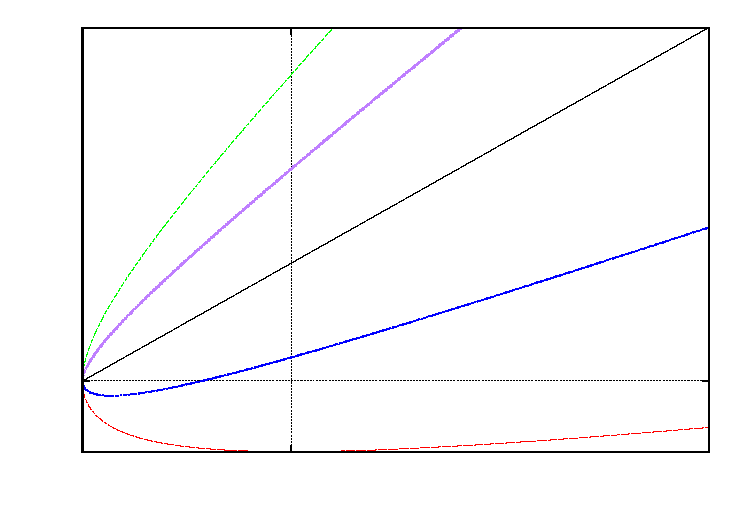
\includegraphics{chapters/neutron_interactions/incoming_outgoing_energies_cm_angle.pdf}}%
    \gplfronttext
  \end{picture}%
\endgroup

  \end{center}
  \caption{\textbf{Outgoing energy from forward reaction as a function of 
      incoming energy and center-of-mass scattering angle cosine}.
    \textit{For fixed incoming energy, there is a one-to-one correspondence
      between outgoing energy and center-of-mass scattering angle cosine. For
      fixed outgoing energy, there is only a one-to-one correspondence
      between incoming energy and center-of-mass scattering angle cosine if the
      outgoing energy is above $\frac{Q}{A(A+1)}$ or if the scattering angle
      cosine is above zero.}}
  \label{fig:in_out_energies_cm}
\end{figure}
\begin{figure}[t!]
  \begin{center}
    % GNUPLOT: LaTeX picture with Postscript
\begingroup
  \makeatletter
  \providecommand\color[2][]{%
    \GenericError{(gnuplot) \space\space\space\@spaces}{%
      Package color not loaded in conjunction with
      terminal option `colourtext'%
    }{See the gnuplot documentation for explanation.%
    }{Either use 'blacktext' in gnuplot or load the package
      color.sty in LaTeX.}%
    \renewcommand\color[2][]{}%
  }%
  \providecommand\includegraphics[2][]{%
    \GenericError{(gnuplot) \space\space\space\@spaces}{%
      Package graphicx or graphics not loaded%
    }{See the gnuplot documentation for explanation.%
    }{The gnuplot epslatex terminal needs graphicx.sty or graphics.sty.}%
    \renewcommand\includegraphics[2][]{}%
  }%
  \providecommand\rotatebox[2]{#2}%
  \@ifundefined{ifGPcolor}{%
    \newif\ifGPcolor
    \GPcolorfalse
  }{}%
  \@ifundefined{ifGPblacktext}{%
    \newif\ifGPblacktext
    \GPblacktexttrue
  }{}%
  % define a \g@addto@macro without @ in the name:
  \let\gplgaddtomacro\g@addto@macro
  % define empty templates for all commands taking text:
  \gdef\gplbacktext{}%
  \gdef\gplfronttext{}%
  \makeatother
  \ifGPblacktext
    % no textcolor at all
    \def\colorrgb#1{}%
    \def\colorgray#1{}%
  \else
    % gray or color?
    \ifGPcolor
      \def\colorrgb#1{\color[rgb]{#1}}%
      \def\colorgray#1{\color[gray]{#1}}%
      \expandafter\def\csname LTw\endcsname{\color{white}}%
      \expandafter\def\csname LTb\endcsname{\color{black}}%
      \expandafter\def\csname LTa\endcsname{\color{black}}%
      \expandafter\def\csname LT0\endcsname{\color[rgb]{1,0,0}}%
      \expandafter\def\csname LT1\endcsname{\color[rgb]{0,1,0}}%
      \expandafter\def\csname LT2\endcsname{\color[rgb]{0,0,1}}%
      \expandafter\def\csname LT3\endcsname{\color[rgb]{1,0,1}}%
      \expandafter\def\csname LT4\endcsname{\color[rgb]{0,1,1}}%
      \expandafter\def\csname LT5\endcsname{\color[rgb]{1,1,0}}%
      \expandafter\def\csname LT6\endcsname{\color[rgb]{0,0,0}}%
      \expandafter\def\csname LT7\endcsname{\color[rgb]{1,0.3,0}}%
      \expandafter\def\csname LT8\endcsname{\color[rgb]{0.5,0.5,0.5}}%
    \else
      % gray
      \def\colorrgb#1{\color{black}}%
      \def\colorgray#1{\color[gray]{#1}}%
      \expandafter\def\csname LTw\endcsname{\color{white}}%
      \expandafter\def\csname LTb\endcsname{\color{black}}%
      \expandafter\def\csname LTa\endcsname{\color{black}}%
      \expandafter\def\csname LT0\endcsname{\color{black}}%
      \expandafter\def\csname LT1\endcsname{\color{black}}%
      \expandafter\def\csname LT2\endcsname{\color{black}}%
      \expandafter\def\csname LT3\endcsname{\color{black}}%
      \expandafter\def\csname LT4\endcsname{\color{black}}%
      \expandafter\def\csname LT5\endcsname{\color{black}}%
      \expandafter\def\csname LT6\endcsname{\color{black}}%
      \expandafter\def\csname LT7\endcsname{\color{black}}%
      \expandafter\def\csname LT8\endcsname{\color{black}}%
    \fi
  \fi
  \setlength{\unitlength}{0.0500bp}%
  \begin{picture}(7200.00,5040.00)%
    \gplgaddtomacro\gplbacktext{%
      \csname LTb\endcsname%
      \put(792,484){\makebox(0,0){\strut{}$\frac{A+1}{A}Q$}}%
      \csname LTb\endcsname%
      \put(2796,484){\makebox(0,0){\strut{}$\frac{A}{A-1}Q$}}%
      \put(572,2739){\rotatebox{-270}{\makebox(0,0){\strut{}Outgoing Energy}}}%
      \put(3797,154){\makebox(0,0){\strut{}Incoming Energy}}%
      \put(6002,765){\makebox(0,0)[l]{\strut{}$^{\mu_{l} = -1}$}}%
      \put(5601,1355){\makebox(0,0)[l]{\strut{}$\mu_{l} = -\frac{1}{2}$}}%
      \put(5200,1925){\makebox(0,0)[l]{\strut{}$\mu_{l} = 0$}}%
      \put(3998,3228){\makebox(0,0)[l]{\strut{}$\mu_{l} = \frac{1}{2}$}}%
      \put(1593,4164){\makebox(0,0)[l]{\strut{}$\mu_{l} = 1$}}%
      \put(632,745){\makebox(0,0)[l]{\strut{}0}}%
    }%
    \gplgaddtomacro\gplfronttext{%
    }%
    \gplbacktext
    \put(0,0){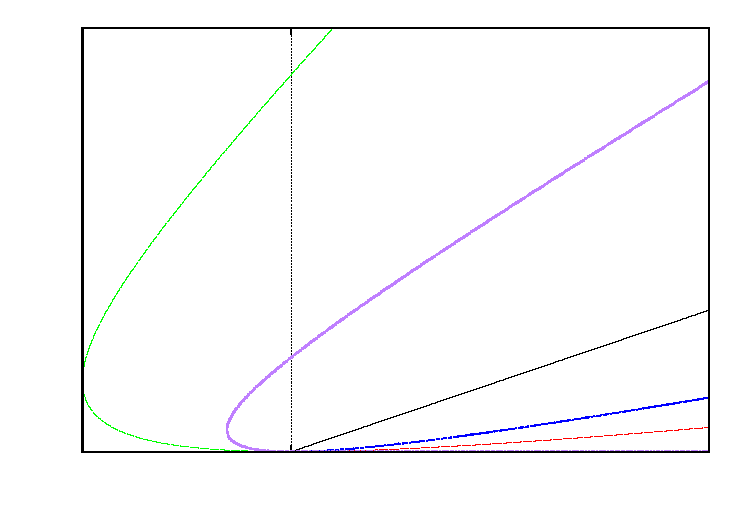
\includegraphics{chapters/neutron_interactions/incoming_outgoing_energies_lab_angle.pdf}}%
    \gplfronttext
  \end{picture}%
\endgroup

  \end{center}
  \caption{\textbf{Outgoing energy from forward reaction as a function of 
      incoming energy and lab scattering angle cosine}.
    \textit{For fixed incoming energy, there is only a one-to-one correspondence
      between outgoing energy and lab scattering angle cosine if the
      incoming energy is above $\frac{AQ}{A-1}$. For fixed outgoing energy,
      there is a one-to-one correspondence between incoming energy and lab
      scattering angle cosine.}}
  \label{fig:in_out_energies_cm}
\end{figure}
The incoming energy as a function of incoming energy and lab scattering angle
cosine is shown in the following equation. It must also be noted that the
primed and unprimed variables have been switched. The derivation of this 
equation is shown in appendix \ref{appendix_C}.
\begin{equation}
  E = E^{'}\left(\frac{A^2-1+2\mu_l^2 + A(A-1)\frac{Q}{E^{'}} - 
    2\mu_l\sqrt{A^2 - 1 + \mu_l^2 + A(A-1)\frac{Q}{E^{'}}}}{(A-1)^2}
  \right)
\end{equation}
By using $\mu_l = 1$ and $\mu_l = -1$ in the above equation, the lower and
upper energy bound of the adjoint elastic and inelastic level scattering
process can be determined, repsectively.
\begin{equation}
  \left(\frac{A\sqrt{1+\left(\frac{A-1}{A}\right)\frac{Q}{E^{'}}}-1}{A-1}
  \right)^2 E^{'} \leq E \leq
  \left(\frac{A\sqrt{1+\left(\frac{A-1}{A}\right)\frac{Q}{E^{'}}}+1}{A-1}
  \right)^2 E^{'}
\end{equation}

With the adjoint cross section for elastic and inelastic level scattering
completely defined, the adjoint energy transfer probability can now be 
determined using equation \ref{eq:adjoint_double_diff_transfer_prob}
\citep{hoogenboom_adjoint_1977}.
\begin{align}
  p^{\dagger}(E^{'} \to E) & = \frac{\sigma_{e/i}(E)p(E \to E^{'})}
  {\sigma_{e/i}^{\dagger}(E^{'})} \nonumber \\
    & = \frac{\sigma_{e/i}(E)}{\sigma_{e/i}^{\dagger}(E^{'})}
  \frac{(A+1)^2}{2AE\sqrt{1-\left(\frac{A+1}{A}\right)\frac{Q}{E}}}
  p(E, \mu_{cm}(E,E^{'})) 
\end{align}
Efficient methods for sampling from this function will be a major focus of this
work. However, it is likely that a tabular method will be used based on the
seemingly complex nature of this PDF.

Because of the one-to-one correspondence between the outgoing energy and
direction, once the outgoing energy has been selected the outgoing direction
is known. The following equation must be used to determine the outgoind
lab scattering angle cosine corresponding to the incoming and outgoing energy.
\begin{equation}
  \mu_l = - \left[\frac{\left(\frac{E}{E^{'}}\right)(A-1)^2 - 
      A^2\left(1+\left(\frac{A-1}{A}\right)\frac{Q}{E^{'}}\right) + 1}
    {2\sqrt{\frac{E}{E^{'}}}(A-1)}\right]
\end{equation}

\section{Other Non-fission Adjoint  Reactions}

\section{Adjoint Neutron Induced Fission}

\section{Adjoint Thermal Scattering}



%\blankpage
%\chapter{Electron Interaction Cross Sections and Sampling Techniques}

%\blankpage
%\include{chapters/positron_interactions/positron_interactions}
%\blankpage
%\chapter{Coupled Neutron and Photon Interaction Cross Sections and Sampling Techniques}

%\blankpage
%\chapter{Coupled Photon, Electron and Positron Interaction Cross Sections and Sampling Techniques}

%% etc, etc.

%% Do you have appendices?  If so, add them here, just like chapters.
\blankpage
\begin{appendices}
\chapter{Alternative Derivation of the Adjoint Emission and Collision Densities}
\label{ch:appendix_a}

In chapter \ref{ch:adjoint_particle_transport}, a FIESK for the adjoint
of the emission density was created. However, it was pointed out that the 
adjoint of the emission density was ``flux-like'' and therefore not ideal to
estimate via a Monte Carlo random walk process. It was also briefly mentioned
that a better function could be constructed if the adjoint of the emission
density was multiplied by some function $\Sigma^{*}(\vec{r},E)$, whose only 
necessary properties are that it is strictly positive and goes to zero in a 
vacuum. In the following sections, two functions will be used to modify the 
adjoint of the emission density. The adjoint of the collision 
density, which is also ``flux-like,'' will also be modified in a similar way.

\section{The Adjoint Collision Density}
\label{sec:adjoint_collision_density}
To derive the adjoint collision density, the adjoint of the emission density
will be multiplied by $\Sigma^{*}(\vec{r},E) = \Sigma_T(\vec{r},E)$, which is 
the total cross section. In the following equation,
$\xi^{\dagger}(\vec{r},E,\hat{\Omega})$ is the adjoint collision density.
\begin{equation}
  \xi^{\dagger}(\vec{r},E,\hat{\Omega}) = \Sigma_T(\vec{r},E)
  \chi^{\dagger}(\vec{r},E,\hat{\Omega})
  \label{eq:adj_collision_dens_to_adjoint_of_emission_dens}
\end{equation}
\begin{align}
  \xi^{\dagger}(\vec{r},E,\hat{\Omega}) & = \int a(\vec{r}^{'},E,\hat{\Omega}) 
  \Sigma_T(\vec{r},E) \tau(\vec{r}^{'},\vec{r},E,-\hat{\Omega}) dV^{'} + 
  \nonumber \\
  \int\int\int  &\frac{\Sigma_T(\vec{r},E)}{\Sigma_T(\vec{r}^{'},E^{'})}
  \tau(\vec{r}^{'},\vec{r},E,-\hat{\Omega}) 
  \Sigma_T(\vec{r}^{'},E \to E^{'},\hat{\Omega} \to \hat{\Omega}^{'})
  \xi^{\dagger}(\vec{r}^{'},E^{'},\hat{\Omega}^{'}) dE^{'}d\hat{\Omega}^{'}dV^{'}
  \nonumber \\
  & = \int a(\vec{r}^{'},E,\hat{\Omega}) 
    T(\vec{r}^{'} \to \vec{r},E,-\hat{\Omega}) dV^{'} + \nonumber \\
    \int\int\int & T(\vec{r}^{'} \to \vec{r},E,-\hat{\Omega})
      \frac{\Sigma_T(\vec{r}^{'},E \to E^{'},\hat{\Omega} \to \hat{\Omega}^{'})}
           {\Sigma_T(\vec{r}^{'},E^{'})}
    \xi^{\dagger}(\vec{r}^{'},E^{'},\hat{\Omega}^{'}) dE^{'}d\hat{\Omega}^{'}dV^{'}
  \nonumber 
\end{align}

As mentioned in chapter \ref{ch:particle_transport}, the transport 
kernel is normalized, assuming that random walks that exit the domain of 
interest are terminated. Interestingly, the particles characterized by the 
adjoint collision density FIESK travel in the direction opposite of the 
variable $\hat{\Omega}$, which is indicated by the negative sign in front of
this variable in the transport kernel. The adjoint transport operator will be
defined as follows.
\begin{equation}
  T^{\dagger}(\vec{r}^{'} \to \vec{r},E,\hat{\Omega}) = 
  T(\vec{r}^{'} \to \vec{r},E,-\hat{\Omega})
  \label{eq:adjoint_transport_kernel}
\end{equation}

The part of the state transition kernel that describes the 
collisions can be normalized to unity by introducing the following factor.
\begin{equation}
  P^{\dagger}(\vec{r}^{'},E^{'}) = 
  \frac{\Sigma^{\dagger}(\vec{r}^{'},E^{'})}{\Sigma_T(\vec{r}^{'},E^{'})}
  \label{eq:adjoint_weight_factor}
\end{equation}
This factor will be called the adjoint weight factor and the function 
$\Sigma^{\dagger}(\vec{r}^{'},E^{'})$ will be called the total macroscopic adjoint 
cross section.
\begin{equation}
  \Sigma^{\dagger}(\vec{r}^{'},E^{'}) = \int\int  
  \Sigma_T(\vec{r}^{'},E \to E^{'},\hat{\Omega} \to \hat{\Omega}^{'}) dE d\Omega
  \label{eq:adjoint_total_cross_section}
\end{equation}
Now the adjoint collision kernel, which is normalized to unity, can be 
defined.
\begin{equation}
  C^{\dagger}(\vec{r}^{'},E^{'} \to E,\hat{\Omega}^{'} \to \hat{\Omega}) = 
  \frac{\Sigma_T(\vec{r}^{'},E \to E^{'},\hat{\Omega} \to \hat{\Omega}^{'})}
       {\Sigma^{\dagger}(\vec{r}^{'},E^{'})}
  \label{eq:adjoint_collision_kernel}
\end{equation}

Using the adjoint transport kernel, adjoint collision kernel and adjoint
weight factor defined, the adjoint collision density state transition kernel
can be defined.
\begin{equation}
  \begin{split}
    N^{\dagger}(\vec{r}^{'} \to \vec{r},E^{'} \to E,\hat{\Omega}^{'} \to \hat{\Omega})
    = T^{\dagger}(\vec{r}^{'} \to \vec{r},E,\hat{\Omega})
    C^{\dagger}(\vec{r}^{'},&E^{'} \to E,\hat{\Omega}^{'} \to \hat{\Omega}) \\
    & \cdot P^{\dagger}(\vec{r}^{'},E^{'})
  \end{split}
\end{equation}

The FIESK for the adjoint collision density can now be written in terms of 
these kernels. In this equation $S_c^{\dagger}(\vec{r},E,\hat{\Omega})$ is the
adjoint first collided source.
\begin{align}
  \xi^{\dagger}(\vec{r},E,\hat{\Omega}) & = \int a(\vec{r}^{'},E,\hat{\Omega}) 
  T^{\dagger}(\vec{r}^{'} \to \vec{r},E,\hat{\Omega}) dV^{'} + \nonumber \\
  \int\int\int &
  N^{\dagger}(\vec{r}^{'} \to \vec{r},E^{'} \to E,\hat{\Omega}^{'} \to \hat{\Omega})
  \xi^{\dagger}(\vec{r}^{'},E^{'},\hat{\Omega}^{'}) dE^{'}d\hat{\Omega}^{'}dV^{'}
  \nonumber \\
  & = S_c^{\dagger}(\vec{r},E,\hat{\Omega}) + \nonumber \\
  \int\int\int &
  N^{\dagger}(\vec{r}^{'} \to \vec{r},E^{'} \to E,\hat{\Omega}^{'} \to \hat{\Omega})
      \xi^{\dagger}(\vec{r}^{'},E^{'},\hat{\Omega}^{'}) dE^{'}d\hat{\Omega}^{'}dV^{'}
  \nonumber
\end{align}

Based on the relationship between the adjoint collision density and the adjoint
of the emission density shown in equation 
\ref{eq:adj_collision_dens_to_adjoint_of_emission_dens}, the inner product must
now be defined as follows.
\begin{equation}
  I = \int\int\int \xi^{\dagger}(\vec{r},E,\hat{\Omega})
  \frac{S(\vec{r},E,\hat{\Omega})}{\Sigma_T(\vec{r},E,\hat{\Omega})}
  dV dE d\hat{\Omega}
\end{equation}
 
\section{The Adjoint ``Collision-Like'' Density}
Another adjoint event density, which is collision-like, can be found in the 
literature \citep{kalos_monte_1968, eriksson_monte_1969}. Instead of 
multiplying the adjoint of the emission density by the total cross section, it 
is multiplied by the total adjoint cross section.
\begin{equation}
  \mu^{\dagger}(\vec{r},E,\hat{\Omega}) = \Sigma^{\dagger}(\vec{r},E)
  \chi^{\dagger}(\vec{r},E,\hat{\Omega})
  \label{eq:adj_collision_like_dens_to_adjoint_of_emission_dens}
\end{equation}
The resulting FIESK for this adjoint ``collision-like'' density is shown below.
In this equation, the definition of the adjoint weight factor, adjoint
transport kernel, adjoint collision kernel and adjoint first collided 
source from the previous section will be used.
\begin{align}
  \mu^{\dagger}(\vec{r},E,\hat{\Omega}) & = \int a(\vec{r}^{'},E,\hat{\Omega}) 
  \Sigma^{\dagger}(\vec{r},E) \tau(\vec{r}^{'},\vec{r},E,-\hat{\Omega}) 
  dV^{'} + \nonumber \\
  \int\int\int  & \frac{\Sigma^{\dagger}(\vec{r},E)}
                       {\Sigma^{\dagger}(\vec{r}^{'},E^{'})}
  \tau(\vec{r}^{'},\vec{r},E,-\hat{\Omega}) 
  \Sigma_T(\vec{r}^{'},E \to E^{'},\hat{\Omega} \to \hat{\Omega}^{'})
  \mu^{\dagger}(\vec{r}^{'},E^{'},\hat{\Omega}^{'}) dE^{'}d\hat{\Omega}^{'}dV^{'}
  \nonumber \\
  & = P^{\dagger}(\vec{r},E) \int
  a(\vec{r}^{'},E,\hat{\Omega}) 
  T(\vec{r}^{'} \to \vec{r},E,-\hat{\Omega}) dV^{'} + \nonumber \\
  \int\int\int &P^{\dagger}(\vec{r},E) 
  T(\vec{r}^{'} \to \vec{r},E,-\hat{\Omega})
  \frac{\Sigma_T(\vec{r}^{'},E \to E^{'},\hat{\Omega} \to \hat{\Omega}^{'})}
       {\Sigma^{\dagger}(\vec{r}^{'},E^{'})}
  \mu^{\dagger}(\vec{r}^{'},E^{'},\hat{\Omega}^{'}) dE^{'}d\hat{\Omega}^{'}dV^{'}
  \nonumber \\
  & = P^{\dagger}(\vec{r},E) 
  S_c^{\dagger}(\vec{r},E,\hat{\Omega}) + \nonumber \\
  \int\int\int &P^{\dagger}(\vec{r},E) 
  T^{\dagger}(\vec{r}^{'} \to \vec{r},E,\hat{\Omega})
  C^{\dagger}(\vec{r}^{'},E^{'} \to E,\hat{\Omega}^{'} \to \hat{\Omega})
  \mu^{\dagger}(\vec{r}^{'},E^{'},\hat{\Omega}^{'}) dE^{'}d\hat{\Omega}^{'}dV^{'}
  \nonumber 
\end{align}

For this adjoint ``collision-like'' density, the state transition kernel is the 
following. 
\begin{equation}
  \begin{split}
    O^{\dagger}(\vec{r}^{'} \to \vec{r},E^{'} \to E,\hat{\Omega}^{'} \to \hat{\Omega})
    = P^{\dagger}(\vec{r},&E) 
    T^{\dagger}(\vec{r}^{'} \to \vec{r},E,\hat{\Omega}) \\
    & \cdot C^{\dagger}(\vec{r}^{'},E^{'} \to E,\hat{\Omega}^{'} \to \hat{\Omega})
  \end{split}
\end{equation}
Interestingly, the only difference between this state transition
kernel and the state transition kernel for the adjoint collision density is
the ordering of the adjoint transport kernel, adjoint collision kernel and the
adjoint weight factor.

Based on the relationship between the adjoint ``collision-like'' density and the
adjoint of the emission density shown in equation 
\ref{eq:adj_collision_like_dens_to_adjoint_of_emission_dens}, the inner product
must now be defined as follows.
\begin{equation}
  I = \int\int\int \mu^{\dagger}(\vec{r},E,\hat{\Omega})
  \frac{S(\vec{r},E,\hat{\Omega})}{\Sigma^{\dagger}(\vec{r},E,\hat{\Omega})}
  dV dE d\hat{\Omega}
\end{equation}

\section{The Adjoint Emission Density}
Using the procedure outlined in chapter \ref{ch:mc_methods}, the adjoint of the
collision density FIESK can be derived. The steps will not be shown, but the 
resulting equation can be seen in the next equation. The function 
$\psi^{\dagger}(\vec{r},E,\hat{\Omega})$ is the adjoint of the collision density.
\begin{align}
  \psi^{\dagger}(\vec{r},E,\hat{\Omega}) & = b(\vec{r},E,\hat{\Omega}) + 
  \nonumber \\
  \int\int\int &C(\vec{r},E \to E^{'},\hat{\Omega} \to \hat{\Omega}^{'})
  T(\vec{r} \to \vec{r}^{'},E^{'},\hat{\Omega}^{'})
  \psi^{\dagger}(\vec{r}^{'},E^{'},\hat{\Omega}^{'}) dV^{'}dE^{'}d\hat{\Omega}^{'}
  \nonumber \\
   & = \frac{a(\vec{r},E,\hat{\Omega})}
            {\Sigma_T(\vec{r},E)}+ \nonumber \\
   \int\int\int & C(\vec{r},E \to E^{'},\hat{\Omega} \to \hat{\Omega}^{'})
   T(\vec{r} \to \vec{r}^{'},E^{'},\hat{\Omega}^{'})
   \psi^{\dagger}(\vec{r}^{'},E^{'},\hat{\Omega}^{'}) dV^{'}dE^{'}d\hat{\Omega}^{'}
   \nonumber
\end{align}

The adjoint of the collision density also exhibits flux-like behavior in that
it will not got to zero in a vacuum. To derive the adjoint emission density,
which will have the desirable property that it goes to zero in a vacuum, the
adjoint of the collision density will be multiplied by the total cross section.
In the following equation $\theta^{\dagger}(\vec{r},E,\hat{\Omega})$ is the
adjoint emission density.
\begin{equation}
  \theta^{\dagger}(\vec{r},E,\hat{\Omega}) = \Sigma_T(\vec{r},E)
  \psi^{\dagger}(\vec{r},E,\hat{\Omega})
  \label{eq:adj_emission_dens_to_adj_of_collision_dens}
\end{equation}
The resulting FIESK for the adjoint emission density is shown below. In this
equation, the definition of the adjoint weight factor, adjoint transport 
kernel and adjoint collision kernel from section 
\ref{sec:adjoint_collision_density} will be used.
\begin{align}
  \theta^{\dagger}(\vec{r},E,\hat{\Omega}) & = a(\vec{r},E,\hat{\Omega}) + 
  \int\int\int \frac{\Sigma_T(\vec{r},E)}{\Sigma_T(\vec{r}^{'},E^{'})}
  C(\vec{r},E \to E^{'},\hat{\Omega} \to \hat{\Omega}^{'}) \nonumber \\
    & \qquad \cdot \Sigma_T(\vec{r}^{'},E^{'})
  \frac{T(\vec{r} \to \vec{r}^{'},E^{'},\hat{\Omega}^{'})}
       {\Sigma_T(\vec{r}^{'},E^{'})}
  \theta^{\dagger}(\vec{r}^{'},E^{'},\hat{\Omega}^{'}) dV^{'}dE^{'}d\hat{\Omega}^{'}
  \nonumber \\
  & = a(\vec{r},E,\hat{\Omega}) + 
  \int\int\int \Sigma_T(\vec{r},E) 
  C(\vec{r},E \to E^{'},\hat{\Omega} \to \hat{\Omega}^{'}) \nonumber \\
  & \qquad \cdot \frac{T(\vec{r}^{'} \to \vec{r},E^{'},-\hat{\Omega}^{'})}
                      {\Sigma_T(\vec{r},E^{'})}
  \theta^{\dagger}(\vec{r}^{'},E^{'},\hat{\Omega}^{'}) dV^{'}dE^{'}d\hat{\Omega}^{'}
  \nonumber \\
  & = a(\vec{r},E,\hat{\Omega}) + 
  \int\int\int \Sigma_T(\vec{r},E \to E^{'},\hat{\Omega} \to \hat{\Omega}^{'}) 
  \nonumber \\
  & \qquad \cdot \frac{T(\vec{r}^{'} \to \vec{r},E^{'},-\hat{\Omega}^{'})}
           {\Sigma_T(\vec{r},E^{'})}
    \theta^{\dagger}(\vec{r}^{'},E^{'},\hat{\Omega}^{'}) dV^{'}dE^{'}d\hat{\Omega}^{'}
  \nonumber \\
  & = a(\vec{r},E,\hat{\Omega}) +
  \int\int\int 
  C^{\dagger}(\vec{r},E^{'} \to E,\hat{\Omega}^{'} \to \hat{\Omega})
  P^{\dagger}(\vec{r},E^{'}) \nonumber \\
  & \qquad \cdot 
  T^{\dagger}(\vec{r}^{'} \to \vec{r},E^{'},\hat{\Omega}^{'})
  \theta^{\dagger}(\vec{r}^{'},E^{'},\hat{\Omega}^{'}) dV^{'}dE^{'}d\hat{\Omega}^{'}
  \nonumber 
\end{align}

For the adjoint emission density, the state transition kernel is the following.
\begin{equation}
  \begin{split}
    M^{\dagger}(\vec{r}^{'} \to \vec{r},E^{'} \to E,\hat{\Omega}^{'} \to \hat{\Omega})
    = C^{\dagger}(\vec{r},E^{'} \to E,&\hat{\Omega}^{'} \to \hat{\Omega})
    P^{\dagger}(\vec{r},E^{'})  \\
    & \cdot T^{\dagger}(\vec{r}^{'} \to \vec{r},E^{'},\hat{\Omega}^{'}) 
  \end{split}
\end{equation}
Again, the only difference between this state transition kernel and the 
previous two is the the ordering of the adjoint transport kernel, adjoint
collision kernel and the adjoint weight factor. 

Based on the relationship between the adjoint emission density and the adjoint
of the collision density shown in equation 
\ref{eq:adj_emission_dens_to_adj_of_collision_dens}, the inner product must now
be defined as follows, where $S_c(\vec{r},E,\hat{\Omega})$ is the first
collided source.
\begin{equation}
  I = \int\int\int \theta^{\dagger}(\vec{r},E,\hat{\Omega})
  \frac{S_c(\vec{r},E,\hat{\Omega})}{\Sigma_T(\vec{r},E,\hat{\Omega})}
  dV dE d\hat{\Omega}
\end{equation}

\blankpage
\chapter{Photon Interaction Physics and Sampling Derivations}
\label{ch:appendix_B}
In chapter \ref{ch:photon_interactions} the derivation of several important
equations were omitted. In this appendix the details of several derivations will
be shown in detail. In particular, the derivation of the outgoing energy of a
photon after a Compton scatter off of a free electron, the electron momentum 
projection on the photon scattering vector from a Compton scatter off of a
bound electron, the Klein-Nishina cross section differential in the inverse
energy loss ratio (x), the total Klein-Nishina cross section, Kahn's
rejection sampling technique, and the pair and triplet production thresholds
will be discussed.

\section{Compton Scattering from Free and Bound Electrons}
The process of Compton scattering off of a free electron is represented by 
figure \ref{fig:compton_scatter_free_electron}. Conservation of energy and 
momentum will be used to determine the final energy of the photon after the 
collision with the electron. First, the momentum of the particle system will be 
analyzed. In the transverse direction, momentum conservation is as follows.
\begin{equation*}
  P\sin{\theta} = P_e\sin{\phi}
\end{equation*}
In the longitudinal direction, momentum conservation is as follows.
\begin{equation*}
  P^{'} = P\cos{\theta} + P_e\cos{\phi} 
\end{equation*}
Both of these equations will now be squared and added together.
\begin{align}
  P^{'2} - 2P^{'}P\cos{\theta} + P^2(cos^2\theta + sin^2\theta) & = 
  P_e^2(cos^2\phi + sin^2\phi) \nonumber \\
  P_e^2 = P^{'2} - 2P^{'}P\cos{\theta} + P^2
\end{align}
This equation for the electron momentum will be useful in the equation for
the conservation of energy of the particle system.

Now, the energy of the particle system will be analyzed. The energy of the
system is shown below.
\begin{equation*}
  E^{'} + m_ec^2 = E + E_e
\end{equation*}
\begin{equation*}
  E^{'}-E + m_ec^2 = E_e
\end{equation*}
\begin{equation*}
  (P^{'} - P)c + m_ec^2 = \sqrt{\left(P_ec\right)^2 + \left(m_ec^2\right)^2}
\end{equation*}
\begin{equation*}
  (P^{'} - P)^2c^2 + 2m_ec^3(P^{'} - P) + m_e^2c^4 = P_e^2c^2 + m_e^2c^4
\end{equation*}
\begin{equation*}
  P^{'2}c^2 - 2P^{'}Pc^2 + P^2c^2 + 2m_ec^3(P^{'} - P) = P^{'2}c^2 - 
  2P^{'}P\cos{\theta}c^2 + P^2c^2
\end{equation*}
\begin{equation*}
  2m_ec^3(P^{'} - P) = 2P^{'}Pc^2(1 - \cos{\theta})
\end{equation*}
\begin{equation*}
  m_ec^3P^{'} = Pc(P^{'}c(1 - \cos{\theta}) + m_ec^2)
\end{equation*}
\begin{align}
  E & = \frac{m_ec^2E^{'}}{E^{'}(1 - \cos{\theta}) + m_ec^2} \nonumber \\
  & = \frac{E^{'}}{1 + \frac{E^{'}}{m_ec^2}(1 - \cos{\theta})} \\
  \alpha & = \frac{\alpha^{'}}{1 + \alpha^{'}(1 - \cos{\theta})} 
\end{align}

\begin{figure}[t!]
  \begin{center}
    \scalebox{1.0}{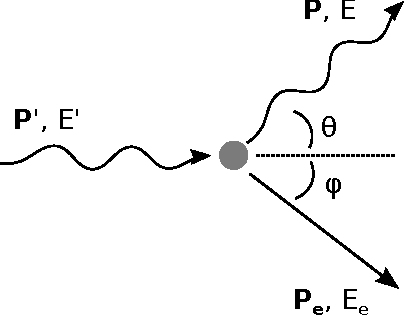
\includegraphics{backmatter/appendix_B/compton_scatter_free_electron.pdf}}
  \end{center}
  \caption{\textbf{Compton scattering off of a free electron.}}
  \label{fig:compton_scatter_free_electron}
\end{figure}

The process of Compton scattering off of a bound electron is represented by
figure \ref{fig:compton_scatter_bound_electron}.
\begin{figure}[t!]
  \begin{center}
    \scalebox{1.0}{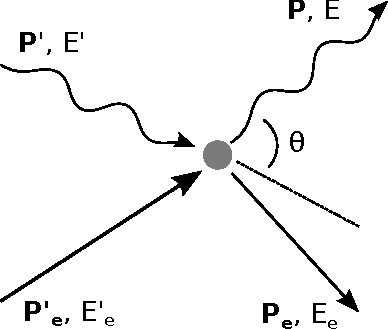
\includegraphics{backmatter/appendix_B/compton_scatter_bound_electron.pdf}}
  \end{center}
  \caption{\textbf{Compton scattering off of a bound electron.}}
  \label{fig:compton_scatter_bound_electron}
\end{figure}
Conservation of energy and momentum will again be used to determine the 
quantity of interest, which in this case is the initial electron momentum, 
$\vec{P_e^{'}}$, projected onto the photon scattering vector, 
$\vec{P} - \vec{P^{'}}$. The z-axis of the system will be set parallel to the
scattering vector. Therefore, the electron momentum projection will be 
represented by the variable $p_z$.

Before analyzing the energy of the particle system, then energy of the 
electron will be discussed. The kinetic energy of the electron will be
represented by, $E_{e,k}$.
\begin{align}
  E_e^2 & = m_e^2c^4 + P_e^2c^2 \nonumber \\
  & = \left(m_ec^2 + E_{e,k}\right)^2 \nonumber
\end{align}
\begin{equation}
  P_e^2c^2 = 2m_ec^2E_{e,k} + E_{e,k}^2
\end{equation}
The energy of the particle system is given below. The binding energy of the 
electron is $E_b$.
\begin{equation*}
  E^{'} + E_{e,k}^{'} + m_ec^2 = E + E_{e,k} + m_ec^2 + E_b
\end{equation*}
\begin{align}
  E^{'}-E-E_b & = E_{e,k} - E_{e,k}^{'} \nonumber \\
  \left(E^{'}-E-E_b\right)^2 & = \left(E_{e,k} - E_{e,k}^{'}\right)^2 \nonumber \\
  & = E_{e,k}^2 - 2E_{e,k}E_{e,k}^{'} + E_{e,k}^{'2} \nonumber \\
  & = P_e^2c^2 - 2m_ec^2E_{e,k} - 2E_{e,k}E_{e,k}^{'} + P_e^{'2}c^2 - 2m_ec^2E_{e,k}^{'}
  \nonumber \\
  & = \left(P_e^2 + P_e^{'2}\right)c^2 - 2m_ec^2E_{e,k}^{'} - 
  2E_{e,k}\left(m_ec^2 + E_{e,k}^{'}\right) \nonumber \\
  & = \left(P_e^2 + P_e^{'2}\right)c^2 - 2m_ec^2E_{e,k}^{'} - 
  2\left(E^{'}-E-E_b+E_{e,k}^{'}\right)\left(m_ec^2 + E_{e,k}^{'}\right) \nonumber\\
  & = \left(P_e^2 + P_e^{'2}\right)c^2 - 4m_ec^2E_{e,k}^{'} - 2E_{e,k}^{'2} -
  2\left(E^{'}-E-E_b\right)\left(m_ec^2 + E_{e,k}^{'}\right) \nonumber \\
  & = \left(P_e^2 - P_e^{'2}\right)c^2 -
  2\left(E^{'}-E-E_b\right)\left(m_ec^2 + E_{e,k}^{'}\right) \nonumber \\
  \left(P_e^2 - P_e^{'2}\right)c^2 & = \left(E^{'}-E-E_b\right)^2 +
  2\left(E^{'}-E-E_b\right)\left(m_ec^2 + E_{e,k}^{'}\right)
\end{align}

The momentum of the particle system will now be analyzed. 
\begin{align}
  \vec{P^{'}} + \vec{P_e^{'}} & = \vec{P} + \vec{P_e} \nonumber \\
  m_ec\vec{\alpha^{'}} + \vec{P_e^{'}} & = m_ec\vec{\alpha} + \vec{P_e} \nonumber
\end{align}
The new variable $\vec{\alpha}$ is simply the momentum of the photon in 
units of $m_ec$. The magnitude of this vector has the following properties.
\begin{align}
  \left|\vec{\alpha}\right| & = \alpha \nonumber \\
  & = \frac{P}{m_ec} \\ 
  & = \frac{E}{m_ec^2} 
\end{align}
The equation for the momentum of the system must be rearranged further before
moving on.
\begin{align}
  \vec{P_e^{'}} - \vec{P_e} & = \vec{q} \nonumber \\
  & = m_ec\left(\vec{\alpha} - \vec{\alpha^{'}}\right) \nonumber
\end{align}
\begin{align}
  q^2 & = (m_ec)^2\left|\vec{\alpha} - \vec{\alpha^{'}}\right| \nonumber \\
  & = (m_ec)^2\left(\alpha^{'2} + \alpha^2 - 
  2\vec{\alpha^{'}}\cdot\vec{\alpha}\right) \nonumber \\
  & = (m_ec)^2\left(\alpha^{'2} + \alpha^2 - 2\alpha^{'}\alpha\cos{\theta}\right)
\end{align}

Now, using the equation for $\vec{q}$, the equation for the electron momentum 
projection can be determined.
\begin{equation*}
  \vec{P_e} = \vec{P_e^{'}} - \vec{q}
\end{equation*}
\begin{equation*}
  P_e^2 = P_e^{'2} + q^2 - 2\vec{P_e^{'}}\cdot\vec{q}
\end{equation*}
\begin{equation*}
  2\vec{P_e^{'}}\cdot\vec{q} = -\left(P_e^2 - P_e^{'2}\right) + q^2
\end{equation*}
\begin{equation*}
  2p_zq = -\left(P_e^2 - P_e^{'2}\right) + q^2 \nonumber
\end{equation*}
\begin{align}
  p_z & = \frac{1}{2q}\left[-\left(P_e^2 - P_e^{'2}\right) + q^2\right] 
  \nonumber \\
  & = \frac{1}{2qc^2}\left[-(E^{'}-E-E_b)^2 - 2(E^{'}-E-E_b)(m_ec^2+E_{e,k}^{'})
    +q^2c^2\right] \nonumber \\
  & = \frac{m_e^2c^4}{2qc^2}\left[
    -\left(\alpha^{'}-\alpha-\frac{E_b}{m_ec^2}\right)^2 -
    2\left(\alpha^{'}-\alpha-\frac{E_b}{m_ec^2}\right)
    \left(1 + \frac{E_{e,k}^{'}}{m_ec^2}\right) + 
    \left|\vec{\alpha} - \vec{\alpha^{'}}\right|^2\right] \nonumber \\
  & = \frac{m_e^2c^2}{2q}\Bigg[-(\alpha^{'}-\alpha)^2 + 
    2(\alpha^{'}-\alpha)\left(\frac{E_b}{m_ec^2}\right) - 
    \left(\frac{E_b}{m_ec^2}\right)^2 -
    2(\alpha^{'}-\alpha)\left(1 + \frac{E_{e,k}^{'}}{m_ec^2}\right) + \nonumber \\
  & \qquad \qquad \qquad
    2\left(\frac{E_b}{m_ec^2}\right)\left(1 + \frac{E_{e,k}^{'}}{m_ec^2}\right) +
    \alpha^{'2} + \alpha^2 - 2\alpha^{'}\alpha\cos{\theta}\Bigg] \nonumber \\
  & = m_ec\frac{\left[(\alpha^{'}-\alpha)\left(1 + \frac{E_{e,k}^{'} - E_b}{m_ec^2}
    \right) + \alpha^{'}\alpha(1-\cos{\theta}) -
    \frac{1}{2}\left(\frac{E_b}{m_ec^2}\right)^2 + 
    \left(\frac{E_b}{m_ec^2}\right)\left(1 + \frac{E_{e,k}^{'}}{m_ec^2}\right)
    \right]} {\sqrt{\alpha^{'2} + \alpha^2 - 2\alpha^{'}\alpha\cos{\theta}}}
\end{align}
If the binding energy and kinetic energy of the electron are assumed to be 
small compared to the rest mass energy of the electron, they can be neglected. 
The resulting equation, which is often reported in the literature is the 
following.
\begin{equation}
  p_z = m_ec\frac{\left[\alpha - \alpha^{'} + \alpha^{'}\alpha(1-\cos{\theta})
      \right]}{\sqrt{\alpha^{'2} + \alpha^2 - 2\alpha^{'}\alpha\cos{\theta}}}
\end{equation}

Derivations that are similar to the ones just shown were completed by Sood
\citep{sood_doppler_2004}. 

\section{The Klein-Nishin Cross Section Differential in Inverse Energy Loss Ratio}
\label{diff_kn_cross_sec_var_change}
As mentioned in chapter \ref{ch:photon_interactions}, the differential 
Klein-Nishina cross section is most easily sampled when a change of variables
from steradians to the inverse energy loss ratio is conducted. The energy loss
ratio, which was originally shown in chapter \ref{ch:photon_interactions}, will
be shown again below.
\begin{align}
  \frac{1}{x} & = \frac{\alpha}{\alpha^{'}} \nonumber \\
  & = \frac{1}{1+\alpha^{'}(1-\cos{\theta})} \nonumber
\end{align}

The change of variables is conducted using the following relationship.
\begin{equation*}
  \frac{d\sigma_{K.N.}(\alpha^{'},x)}{dx} dx = 
  \frac{d\sigma_{K.N.}(\alpha^{'},\theta)}{d\Omega} d\Omega
\end{equation*}
\begin{equation*}
  \frac{d\sigma_{K.N.}(\alpha^{'},x)}{dx} = 
  \frac{d\sigma_{K.N.}(\alpha^{'},\theta)}{d\Omega}
  \left(\frac{d\Omega}{dx}\right)
\end{equation*}
Based on the equation for the energy loss ratio, the second term in the above
equation can be determined.
\begin{align}
  x = 1 + \alpha^{'}(1-\cos{\theta}) \nonumber \\
  dx = -\alpha^{'} d(\cos{\theta}) \nonumber
\end{align}
\begin{align}
  \frac{d\Omega}{dx} & = -2\pi\frac{d(\cos{\theta})}{dx} \nonumber \\
  & = \frac{2\pi}{\alpha^{'}}
\end{align}
The following relationships will also be useful while conducting the change
of variables.
\begin{align}
  x - 1 & = \alpha^{'}(1-\cos{\theta}) \\
  cos^2\theta & = 1 - \frac{2(x-1)}{\alpha^{'}} + \frac{(x-1)^2}{\alpha^{'2}}
\end{align}
Now, the change of variables can be completed.
\begin{align}
  \frac{d\sigma_{K.N.}(\alpha^{'},x)}{dx} & = \frac{r_e^2}{2}
  \frac{\left[1 + \cos{^{2}\theta} + \frac{\alpha^{'2}(1-\cos{\theta})^2}
                                  {1 + \alpha^{'}(1-\cos{\theta})}\right] }
  {\left[1 + \alpha^{'}(1-\cos{\theta}) \right]^2} 
  \left(\frac{2\pi}{\alpha^{'}}\right) \nonumber \\
  & = \left(\frac{\pi r_e^2}{\alpha^{'}x^2}\right)
  \left[1 + 
    \left(1 - \frac{2(x-1)}{\alpha^{'}} + \frac{(x-1)^2}{\alpha^{'2}}\right) +
    \frac{(x-1)^2}{x} \right] \nonumber \\
  & = \left(\frac{\pi r_e^2}{\alpha^{'}x^2}\right) \left[2 - 
    \frac{2x}{\alpha^{'}} + \frac{2}{\alpha^{'}} +\frac{x^2}{\alpha^{'2}} -
    \frac{2x}{\alpha^{'2}} + \frac{1}{\alpha^{'2}} + x - 2 + \frac{1}{x} \right]
  \nonumber \\
  & = \left(\frac{\pi r_e^2}{\alpha^{'}}\right) \left[ \frac{1}{\alpha^{'2}} +
    \frac{1}{x}\left(1 - \frac{2}{\alpha^{'}}-\frac{2}{\alpha^{'2}}\right) +
    \frac{1}{x^2}\left(\frac{2}{\alpha^{'}} + \frac{1}{\alpha^{'2}}\right) +
    \frac{1}{x^3} \right] \nonumber \\
  & = K \left[A + \frac{B}{x} + \frac{C}{x^2} + \frac{D}{x^3}\right]
\end{align}
\begin{align}
  K & = \frac{\pi r_e^2}{\alpha^{'}} \nonumber \\
  A & = \frac{1}{\alpha^{'}} \nonumber \\
  B & = 1 - \frac{2(\alpha^{'}+1)}{\alpha^{'2}} \nonumber \\
  C & = \frac{(1+2\alpha^{'})}{\alpha^{'2}} \nonumber \\
  D & = 1 \nonumber 
\end{align}

\section{The Total Klein-Nishina Cross Section}
Using the sampling methods from chapter \ref{ch:photon_interactions} will 
sometimes require the total Klein-Nishina cross section. Using the 
Klein-Nishina cross section differential in the inverse energy loss ratio,
the total Klein-Nishina cross section can be determined rather easily. The
integration of the differential cross section will be split up into four parts
and then recombined and reorganized to give the total cross section reported by 
Lux (with the error corrected) \citep{lux_monte_1991}. 
\begin{align}
  \sigma_{K.N.}(\alpha^{'}) & = \int_1^{1+2\alpha^{'}} \frac{d\sigma_{K.N.}(x)}{dx} dx
  \nonumber \\
  & = K \left(\int_1^{1+2\alpha^{'}} A dx + 
    \int_1^{1+2\alpha^{'}} \frac{B}{x} dx + 
    \int_1^{1+2\alpha^{'}} \frac{C}{x^2} dx + 
    \int_1^{1+2\alpha^{'}} \frac{D}{x^3} dx \right) \nonumber \\
  & = K \left(Ax \Bigg|_1^{1+2\alpha^{'}} + B\ln{x}\Bigg|_1^{1+2\alpha^{'}} -
    \frac{C}{x} \Bigg|_1^{1+2\alpha^{'}} - \frac{D}{2x^2} \Bigg|_1^{1+2\alpha^{'}}
    \right) \nonumber \\
  & = K \left(2\alpha^{'}A + B\ln{(1+2\alpha^{'})} - \frac{C}{1+2\alpha^{'}} + C -
    \frac{D}{2(1+2\alpha^{'})^2} + \frac{D}{2} \right) \nonumber \\
  & = K \left(\frac{2}{\alpha^{'}} + \ln{(1 + 2\alpha^{'})} -
    \frac{2(\alpha^{'}+1)}{\alpha^{'2}}\ln{(1+2\alpha^{'})} - 
    \frac{1}{\alpha^{'2}} + \frac{1+2\alpha^{'}}{\alpha^{'2}} - 
    \frac{1}{2(1+2\alpha^{'2})^2} + \frac{1}{2} \right) \nonumber \\
  & = K \left(\frac{2}{\alpha^{'}} + \ln{(1 + 2\alpha^{'})} -
    \frac{2(\alpha^{'}+1)}{\alpha^{'2}}\ln{(1+2\alpha^{'})} + 
    \frac{2}{\alpha^{'}} + \frac{2\alpha^{'}(1+\alpha^{'})}{(1+2\alpha^{'})^2} 
    \right) \nonumber \\
  & = K \left(\frac{4(1+\alpha^{'})^2}{\alpha^{'}(1+2\alpha^{'})} - 
      \frac{4\alpha^{'}}{1+2\alpha^{'}} + \ln{(1 + 2\alpha^{'})} -
    \frac{2(\alpha^{'}+1)}{\alpha^{'2}}\ln{(1+2\alpha^{'})} + 
    \frac{2\alpha^{'}(1+\alpha^{'})}{(1+2\alpha^{'})^2} 
    \right) \nonumber \\
  & = K \left(\frac{2(1+\alpha^{'})}{\alpha^{'}} 
    \left[\frac{2(1+\alpha^{'})}{1+2\alpha^{'}} - 
    \frac{\ln{(1+2\alpha^{'})}}{\alpha^{'}} \right] + \ln{(1 + 2\alpha^{'})} -
    \frac{4\alpha^{'}}{1+2\alpha^{'}} + 
    \frac{2\alpha^{'}(1+\alpha^{'})}{(1+2\alpha^{'})^2} \right) \nonumber \\
  & = K \left(\frac{2(1+\alpha^{'})}{\alpha^{'}} 
    \left[\frac{2(1+\alpha^{'})}{1+2\alpha^{'}} - 
    \frac{\ln{(1+2\alpha^{'})}}{\alpha^{'}} \right] + \ln{(1 + 2\alpha^{'})} -
    \frac{2\alpha^{'}(1+3\alpha^{'})}{(1+2\alpha^{'})^2} \right) \nonumber \\
  & = 2\pi r_e^2 \left(\frac{(1+\alpha^{'})}{\alpha^{'2}} 
    \left[\frac{2(1+\alpha^{'})}{1+2\alpha^{'}} - 
    \frac{\ln{(1+2\alpha^{'})}}{\alpha^{'}} \right] +
    \frac{\ln{(1 + 2\alpha^{'})}}{2\alpha^{'}} - 
    \frac{(1+3\alpha^{'})}{(1+2\alpha^{'})^2} \right) 
\end{align}

In the equation for the total Klein-Nishina cross section reported by Lux, the
second and third terms have an error \citep{lux_monte_1991}. The second term is
\begin{equation*}
  \frac{\ln{(1 + 2\alpha^{'})}}{2\alpha^{'}}.
\end{equation*}
In the equation reported by Lux, this term is
\begin{equation*}
  \frac{\ln{(1 + 2\alpha^{'})}}{2\alpha^{'2}}.
\end{equation*}
The third term is 
\begin{equation*}
  -\frac{(1+3\alpha^{'})}{(1+2\alpha^{'})^2}.
\end{equation*}
In the equation reported by Lux, this term is
\begin{equation*}
  -\frac{(1+3\alpha^{'})}{\alpha^{'}(1+2\alpha^{'})^2}.
\end{equation*}

\section{Kahn's Klein-Nishina Rejection Sampling Procedure}
\label{sec:Kahn_rejection_procedure_der}
As mentioned in chapter \ref{ch:photon_interactions}, below an incoming photon
energy of about 1.4 MeV, Kahn's rejection sampling procedure must be used to
sample the outgoing angle and energy of the photon after a Compton scattering
event. In this section, the derivation of this rejection sampling procedure will
be presented. First, rejection sampling must be explained. 

Most PDFs can be expanded in the following way.
\begin{equation}
  p(x) = \frac{\sum_i^m p_i T_i(x)n_i(x)}{\kappa}
  \label{eq:general_pdf_expansion}
\end{equation}
The number of factors, $m$, is arbitrary although splitting a PDF into more than
one factor can improve the sampling efficiency \citep{kahn_applications_1956}.
The probability of selecting a value of x from a particular factor is $p_i$.
The function $T_i(x)$ must be bounded in the interval (0,1). The efficiency
of the sampling procedure is $\kappa$. Now, to sample a value of $x$, one 
first samples an index $i$ from the disctrete PDF $p(i) = p_i$. Then, one 
samples a value of $x$ from the PDF $n_i(x)$. Finally, if the following 
equality holds, the value is accepted. Otherwise the entire process is repeated.
The quantity $\varepsilon$ is a uniform random number in the interval (0,1).
\begin{equation*}
  \varepsilon \leq T_i(x)
\end{equation*}

The simplest possible expansion for rejection sampling would be the following.
\begin{equation*}
  \kappa p(x) = \left(\frac{p(x)}{C}\right)\left(\frac{1}{b-a}\right)
\end{equation*}
Using this expansion, one would sample a value of x from the uniform 
distribution in the interval (a,b). Then the rejection function $\frac{p(x)}{C}$
would be used to determine if x should be accepted or rejected. The value of
C is simply the maximum value of the PDF $p(x)$.

Often, determining the expansion with the largest efficiency requires trial and
error as many possible expansions can exist for each PDF. This is the case with
the PDF corresponding to the differential Klein-Nishina cross section. Only the 
optimum expansion will be shown.

To begin, the PDF corresponding to the differential Klein-Nishina cross section 
will be derived. A change of variables to the inverse energy loss ratio must
be conducted first, which is shown in section 
\ref{diff_kn_cross_sec_var_change}.
\begin{equation*}
  \frac{d\sigma_{K.N.}(\alpha^{'},x)}{dx} = \frac{\pi r_e^2}{\alpha^{'}x^2}
  \left(\frac{1}{x} + x - 1 + cos^2\theta \right)
\end{equation*}
The PDF corresponding to this cross section is simply
\begin{align}
  p(\alpha^{'},x) & = 
  \begin{cases}
    \frac{1}{K(\alpha^{'})x^2}\left(\frac{1}{x} + x - 1 + cos^2\theta \right)
    & \text{if } 1 \leq x \leq 1 + 2\alpha^{'} \\
    0 & \text{o.w.}
  \end{cases} \\
  K(\alpha^{'}) & = \int_1^{1+2\alpha^{'}} \frac{dx}{x^2}
  \left(\frac{1}{x}+x-1+cos^2\theta \right) \nonumber \\
  & = \left(\frac{\alpha^{'}}{\pi r_e^2}\right) \sigma_{K.N}(\alpha^{'})
\end{align}

Now, the PDF will be factored into the following form.
\begin{equation*}
  \kappa p(\alpha^{'},x) = p_1(\alpha^{'})T_1(\alpha^{'},x)n_1(\alpha^{'},x) + 
  p_2(\alpha^{'})T_2(\alpha^{'},x)n_2(\alpha^{'},x)
\end{equation*}
The first factor $T_1(\alpha^{'},x)n_1(\alpha^{'},x)$ will have the following 
form.
\begin{equation*}
  T_1(\alpha^{'},x)n_1(\alpha^{'},x) = C_1(\alpha^{'})\left(\frac{1}{x} - 
  \frac{1}{x^2}\right)
\end{equation*}
The most efficient way to sample from this distribution is to sample a value
of x from the uniform distribution.
\begin{equation}
  n_1(\alpha^{'},x) = \frac{1}{2\alpha^{'}}
\end{equation}
The rejection function is then
\begin{equation*}
  T_1(\alpha^{'},x) = C_{T1}\left(\frac{1}{x} - \frac{1}{x^2}\right).
\end{equation*}
This function evaluates to zero when $x = 1$. The maximum value of this function
occurs when $x = 2$. Therefore, $C_{T1}$ must equal four so that the function
is always between zero and one.
\begin{equation}
  T_1(\alpha^{'},x) = 4\left(\frac{1}{x} - \frac{1}{x^2}\right).
\end{equation}

The second factor $T_2(\alpha^{'},x)n_2(\alpha^{'},x)$ will have the following 
form.
\begin{equation*}
  T_2(\alpha^{'},x)n_2(\alpha^{'},x) = \frac{C_2(\alpha^{'})}{x^2}
  \left(cos^2\theta + \frac{1}{x}\right)
\end{equation*}
The most efficienct way to sample from this distribution is to sample a value
of x from the follwing distribution.
\begin{equation}
  n_2(\alpha^{'},x) = \frac{1+2\alpha^{'}}{2\alpha^{'} x^2}
\end{equation}
The rejection function is then
\begin{equation*}
  T_2(\alpha^{'},x) = C_{T2}\left(cos^2\theta + \frac{1}{x} \right)
\end{equation*}
The maximum value of this function occurs when x equals unity and 
correspondingly, $\cos{\theta}$ equals unity. To ensure that this function is
always between zero and one, $C_{T2} = \frac{1}{2}$.
\begin{equation}
  T_2(\alpha^{'},x) = \frac{1}{2}\left(cos^2\theta + \frac{1}{x} \right)
\end{equation}

Now, the probabilities associated with each factor need to be determined.
\begin{equation*}
  \kappa p(\alpha^{'},x) = \frac{2 p_1(\alpha^{'})}{\alpha^{'}}
  \left(\frac{1}{x} - \frac{1}{x^2}\right) + 
  \frac{1+2\alpha^{'}}{4\alpha^{'}x^2}p_2 \left(cos^2\theta + \frac{1}{x}\right)
\end{equation*}
\begin{align}
  \frac{2p_1}{\alpha^{'}} & = \frac{1+2\alpha^{'}}{4\alpha^{'}}p_2 \nonumber \\
  & = \frac{1+2\alpha^{'}}{4\alpha^{'}}(1-p_1) \nonumber \\
  p_1\left(\frac{2}{\alpha^{'}} + \frac{1}{4\alpha^{'}} + \frac{1}{2} \right)
  & = \frac{1+2\alpha^{'}}{4\alpha^{'}} \nonumber \\
  p_1 = \frac{1+2\alpha^{'}}{9 + 2\alpha^{'}} \\
  p_2 = \frac{8}{9 + 2\alpha^{'}}
\end{align}
The efficiency associated with this rejection scheme is
\begin{equation}
  \kappa(\alpha^{'}) = \frac{2 K(\alpha^{'})(1+2\alpha^{'})}
  {\alpha^{'}(2\alpha^{'}+9)}.
\end{equation}

Kahn's rejection sampling procedure corresponds to the above expansion.
  
\section{The Adjoint Klein-Nishina Cross Section Differential in Inverse Energy Gain Ratio}
In this section, the derivation of the adjoint Klein-Nishina cross section
differential in inverse energy gain ratio will be shown. The energy gain
ratio, which was originally shown in chapter \ref{ch:photon_interactions}, 
will be shown again.
\begin{align}
  \frac{1}{x} & = \frac{\alpha}{\alpha^{'}} \nonumber \\
  & = \frac{1}{1 - \alpha^{'}(1-\cos{\theta})} \nonumber
\end{align}

The change of variables is conducted using the following relationship.
\begin{align}
  \frac{d\sigma_{K.N.}^{\dagger}(\alpha^{'},x)}{dx}dx & =
  \frac{d\sigma_{K.N.}^{\dagger}(\alpha^{'},\theta)}{dE}dE \nonumber \\
  \frac{d\sigma_{K.N.}^{\dagger}(\alpha^{'},x)}{dx} & = 
  \frac{d\sigma_{K.N.}^{\dagger}(\alpha^{'},\theta)}{dE} \left|\frac{dE}{dx}\right|
  \nonumber
\end{align}
Based on the equation for the energy gain ratio, the second term in the above
equation can be determined.
\begin{align}
  x = \frac{\alpha^{'}}{\alpha} \nonumber \\
  dx = -\frac{\alpha^{'}}{\alpha^2}d\alpha \nonumber
\end{align}
\begin{align}
  \frac{dx}{dE} & = -\frac{\alpha^{'}}{\alpha^2}\frac{d\alpha}{dE} \nonumber \\
  & = -\frac{\alpha^{'}}{m_ec^2\alpha^2}
\end{align}
The following relationship will also be useful while conducting the change
of variables.
\begin{equation}
  cos^2\theta = 1 - \frac{2(1-x)}{\alpha^{'}} + \frac{(1-x)^2}{\alpha^{'2}}
\end{equation}
Now the change of variables can be completed.
\begin{align}
  \frac{d\sigma_{K.N.}^{\dagger}(\alpha^{'},x)}{dx} & = 
  \frac{\pi r_e^2}{m_ec^2 \alpha^2}\left[x + \frac{1}{x} 
    - 1 + cos^2\theta \right] \left(\frac{m_ec^2\alpha^2}{\alpha^{'}}\right) 
  \nonumber \\
  & = \frac{\pi r_e^2}{\alpha^{'}} \left[x + \frac{1}{x} - 1 + cos^2\theta 
    \right] \\
  & = \frac{\pi r_e^2}{\alpha^{'}} \left[x + \frac{1}{x} - 1 + 1 - 
    \frac{2(1-x)}{\alpha^{'}} + \frac{(1-x)^2}{\alpha^{'2}} \right] \nonumber \\
  & = \frac{\pi r_e^2}{\alpha^{'}} \left[x + \frac{1}{x} - \frac{2}{\alpha^{'}} 
    + \frac{2x}{\alpha^{'}} + \frac{1}{\alpha^{'2}} - \frac{2x}{\alpha^{'2}} + 
    \frac{x^2}{\alpha^{'2}} \right] \nonumber \\
  & = \frac{\pi r_e^2}{\alpha^{'}} \left[\frac{1}{x} + 
    x\left(1 + \frac{2}{\alpha^{'}} - \frac{2}{\alpha^{'2}}\right) +
    x^2\left(\frac{1}{\alpha^{'2}}\right) - \frac{2}{\alpha^{'}} + 
    \frac{1}{\alpha^{'2}} \right] \nonumber \\
  & = K^{\dagger}\left[A^{\dagger}x^2 + B^{\dagger}x + C^{\dagger} + 
    \frac{D^{\dagger}}{x} \right]
\end{align}
\begin{align}
  K^{\dagger} & = \frac{\pi r_e^2}{\alpha^{'}} \nonumber \\
  A^{\dagger} & = \frac{1}{\alpha^{'2}} \nonumber \\
  B^{\dagger} & = 1 + \frac{2(\alpha^{'}-1)}{\alpha^{'2}} \nonumber \\
  C^{\dagger} & = \frac{1-2\alpha^{'}}{\alpha^{'2}} \nonumber \\
  D^{\dagger} & = 1 \nonumber
\end{align}
  
\section{Efficient Adjoint Klein-Nishina Rejection Sampling Procedure}
As explained in section \ref{sec:Kahn_rejection_procedure_der} and shown in
equation \ref{eq:general_pdf_expansion}, a PDF can be split into many factors 
from which values of the PDF are sampled. In the case of the PDF corresponding 
to the differential adjoint Klein-Nishina cross section, three factors will 
used. 
\begin{align}
  \kappa p_{K.N.}^{\dagger}(x|\alpha^{'},\alpha_{max}) & = 
  p_1(\alpha^{'},\alpha_{max})T_1(\alpha^{'},\alpha_{max},x)
  n_1(\alpha^{'},\alpha_{max},x) \nonumber \\
  & \quad + p_2(\alpha^{'},\alpha_{max})T_2(\alpha^{'},\alpha_{max},x)
  n_2(\alpha^{'},\alpha_{max},x) \nonumber \\
  & \quad + p_3(\alpha^{'},\alpha_{max})T_3(\alpha^{'},\alpha_{max},x)
  n_3(\alpha^{'},\alpha_{max},x) \nonumber 
\end{align}
The PDF corresponding to the differential adjoint Klein-Nishina cross section 
was shown in equation \ref{eq:reorganized_adjoint_KN_pdf}. It will be shown 
here again for convenience.
\begin{equation}
  p_{K.N.}^{\dagger}(x|\alpha^{'},\alpha_{max}) = 
  \begin{cases}
    H^{\dagger}\left[\left(\frac{1}{x} - 1 \right) + \left(x\right) + 
      \left(cos^2\theta\right) \right] 
    & \text{if } x_{min} \leq x \leq 1 \\
    0 & \text{o.w.}
  \end{cases}
\end{equation}
The three terms from which the three factors will be derived are shown in
parenthesis in the above equation. 

The first factor $T_1(\alpha^{'},\alpha_{max},x)n_1(\alpha^{'},\alpha_{max},x)$
will have the following form.
\begin{equation*}
  T_1(\alpha^{'},\alpha_{max},x)n_1(\alpha^{'},\alpha_{max},x) = 
  C_1(\alpha^{'},\alpha_{max})\left(\frac{1}{x}-1\right)
\end{equation*}
The most efficient way to sample from this distribution is to sample a value of
x from the following distribution.
\begin{equation}
  n_1(\alpha^{'},\alpha_{max},x) = -\frac{1}{x\ln{x_{min}}}
\end{equation}
The rejection function is then 
\begin{equation*}
  T_1(\alpha^{'},\alpha_{max},x) = C_{T1}(\alpha^{'},\alpha_{max})(1-x).
\end{equation*}
This function evaluates to zero when $x=1$. The maximum value of this function
occurs when $x=x_{min}$. Therefore, this function must be defined as follows.
\begin{equation}
  T_1(\alpha^{'},\alpha_{max},x) = \frac{1-x}{1-x_{min}}
\end{equation}

The second factor $T_2(\alpha^{'},\alpha_{max},x)n_2(\alpha^{'},\alpha_{max},x)$
will have the following form.
\begin{equation*}
  T_2(\alpha^{'},\alpha_{max},x)n_2(\alpha^{'},\alpha_{max},x) = 
  C_2(\alpha^{'},\alpha_{max})x
\end{equation*}
This distribution can be sampled from directly. Therefore a value of x will
be sampled from the following distribution.
\begin{equation}
  n_2(\alpha^{'},\alpha_{max},x) = \frac{2x}{1-x_{min}^2}
\end{equation}
The rejection function is then simply unity due to the direct sampling.

The third factor $T_3(\alpha^{'},\alpha_{max},x)n_3(\alpha^{'},\alpha_{max},x)$
will have the following form.
\begin{align}
  T_3(\alpha^{'},\alpha_{max},x)n_3(\alpha^{'},\alpha_{max},x) & = 
  C_3(\alpha^{'},\alpha_{max})cos^2\theta \nonumber \\
  & = C_3(\alpha^{'},\alpha_{max})
  \left(1 - \frac{1}{\alpha^{'}} + \frac{x}{\alpha^{'}}\right)^2 \nonumber \\
  & = \frac{C_3(\alpha^{'},\alpha_{max})}{\alpha^{'2}}\left(x-1+\alpha^{'}\right)^2
  \nonumber \\
\end{align}
This distribution can also be sampled from directly. Therefore a value of x
will be sampled from the following distribution.
\begin{equation}
  n_3(\alpha^{'},\alpha_{max},x) = \frac{3\left(x-1+\alpha^{'}\right)^2}
  {\alpha^{'3} - \left(x_{min}-1+\alpha^{'}\right)^3}
\end{equation}
The rejection function will again be simply unity due to the direct sampling.

Now the probabilities associated with each factor need to be determined.
\begin{align}
  \kappa p_{K.N.}^{\dagger}(x|\alpha^{'},\alpha_{max}) & = 
  -\frac{p_1(\alpha^{'},\alpha_{max})}{x\ln{x_{min}}}
  \left(\frac{1-x}{1-x_{min}}\right) +
  \frac{2xp_2(\alpha^{'},\alpha_{max})}{1-x_{min}^2} \nonumber \\
  & \quad +
  \frac{3p_3(\alpha^{'},\alpha_{max})\left(x-1+\alpha^{'}\right)^2}
  {\alpha^{'3} - \left(x_{min}-1+\alpha^{'}\right)^3} \nonumber
\end{align}

\begin{align}
  \frac{2p_2(\alpha^{'},\alpha_{max})}{1-x_{min}^2} & = 
  -\frac{p_1(\alpha^{'},\alpha_{max})}{\ln{x_{min}}\left(1-x_{min}\right)} \\
  \frac{2p_2(\alpha^{'},\alpha_{max})}{1-x_{min}^2} & = 
  \frac{3\alpha^{'2}p_3(\alpha^{'},\alpha_{max})}
       {\alpha^{'3} - \left(x_{min}-1+\alpha^{'}\right)^3} \\
  1 = p_1(\alpha^{'},\alpha_{max}) & + p_2(\alpha^{'},\alpha_{max}) +
  p_3(\alpha^{'},\alpha_{max})
\end{align}
By solving the above system of equations, the probabilities can be determined, 
which are shown below.
\begin{align}
  p_1(\alpha^{'},\alpha_{max}) & = 
  -\frac{3\ln{x_{min}}\left(1-x_{min}\right)\alpha^{'2}}
  {\frac{3}{2}\left(1-x_{min}^2\right)\alpha^{'2} - 
    3\ln{x_{min}}\left(1-x_{min}\right)\alpha^{'2} + \alpha^{'3} - 
    \left(x_{min}-1+\alpha^{'}\right)^3} \\
  p_2(\alpha^{'},\alpha_{max}) & = 
  \frac{\frac{3}{2}\left(1-x_{min}^2\right)\alpha^{'2}}
  {\frac{3}{2}\left(1-x_{min}^2\right)\alpha^{'2} - 
    3\ln{x_{min}}\left(1-x_{min}\right)\alpha^{'2} + \alpha^{'3} - 
    \left(x_{min}-1+\alpha^{'}\right)^3} \\
  p_3(\alpha^{'},\alpha_{max}) & =
  \frac{\alpha^{'3} - \left(x_{min}-1+\alpha^{'}\right)^3}
  {\frac{3}{2}\left(1-x_{min}^2\right)\alpha^{'2} - 
    3\ln{x_{min}}\left(1-x_{min}\right)\alpha^{'2} + \alpha^{'3} - 
    \left(x_{min}-1+\alpha^{'}\right)^3}
\end{align}
The efficiency associated with this rejection scheme is 
\begin{align}
  \kappa(\alpha^{'}&,\alpha_{max}) = 
  \frac{\alpha^{'}\sigma_{K.N.}^{\dagger}(\alpha^{'},\alpha_{max})}{\pi r_e^2}
  \nonumber \\
  &\cdot \left(\frac{3\alpha^{'2}}{\frac{3}{2}\left(1-x_{min}^2\right)\alpha^{'2} 
    -3\ln{x_{min}}\left(1-x_{min}\right)\alpha^{'2} + \alpha^{'3} - 
    \left(x_{min}-1+\alpha^{'}\right)^3}\right)
\end{align}
  

\end{appendices}

%% Are you a big nerd with a colophon?  Add it here.
%% \begin{colophon}
%% \svnidlong{$LastChangedBy$}{$LastChangedRevision$}{$LastChangedDate$}{$HeadURL: http://freevariable.com/dissertation/trunk/frontmatter.tex $}
\vcinfo{}

This template uses Gyre Pagella by default.  (I used Arno Pro in my dissertation.)

Feel free to give me a shout-out in your colophon or acks if this template is useful for you.  Good luck!

%% \end{colophon}

%% McBride is a very nice style (some version is included in this
%% distribution)
\blankpage
\bibliographystyle{mcbride}
\bibliography{references}

%% Want an index?  Neither did I.
\printindex

\end{document}
